\section{Analysis\label{sec:analysis}}

To study the effect of radiation damage on scintillation yield, the laser response in each tile was measured periodically as the total integrated dose accumulated. Thus it is necessary to relate the relative light yield of each tile in a given run to its absorbed dose, rather than the delivered luminosity. The integrated luminosities at the time of each measurement were converted to integrated doses based on film dosimetry measurements in the CRF performed in 2015~\cite{CMS-DN-2018-008}. After a total integrated luminosity of 10.03 \fbinv, the closest tiles to the beam received a dose of approximately 6.04 Mrad, while the farthest tiles received a dose of approximately 1.53 Mrad.
%N.B. The max and min total doses quoted here are for SCSN81 tiles only.
%The remaining relative light yield as a function of dose for a selection of channels is shown in Figure~\ref{remaining_relative_dose}.

\subsection{Analysis procedure\label{sec:ana-proc}} 

In each event, the laser response in each channel is characterized by summing the charge collected in a window of 4 time slices around the pulse peak, beginning with the time slice immediately before the peak time slice and continuing through the two time slices after the peak. The first two time slices in the readout window are always avoided since they sometimes contained huge spikes due to a firmware bug present during data-taking. Since the SiPM+QIE11 pedestal currents are non-neglible and also grow with total received dose, average pedestals for each channel and capacitor were measured at the time of each laser run and subtracted from the charge observed during the laser pulses. Example average pulse shapes and pedestals can be seen in Figures~\ref{pulse0ifb},~\ref{pulse2p7ifb} and~\ref{pulse9p5ifb} for a selection of channels at various doses. This pedestal-subtracted pulse size integrated over four time slices is a measure of the tile's light yield.

During each dedicated laser run, the laser is fired into the CRF tiles 10000 times. Thus, for a given run, the light yield of a tile is taken as the mean of the distribution of 10000 pedestal-subtracted pulse size measurements. This figure is then divided by the mean light yield of the reference tile in that same run to factor out run-to-run variation due to the laser amplitude; this will be referred to as the normalized light yield L.% The charge progressions before and after normalization to the reference tile are shown in Figures~\ref{energy_raw} and Figures~\ref{energy_norm}.
%%The resulting relative charge progressions over X \fbinv are shown in Fig...

To assess the drop in light yield L(\textit{d}) of a tile relative after dose \textit{d} to its pre-irradiation light yield taken on day 0 (defined as the day when the tiles were installed on the CASTOR table), the normalized light yield of the tile is divided by the normalized light yield L(0) from day 0, to yield the relative light yield L(\textit{d})/L(0) as expressed in Equation~\ref{eq:lightloss}. L(\textit{d})/L(0) is plotted as a function of dose in order to calculate the dose constant for a tile.
%These ratios are shown in Figure~\ref{remaining_relative}.

\begin{figure}[tbp!]
\centering
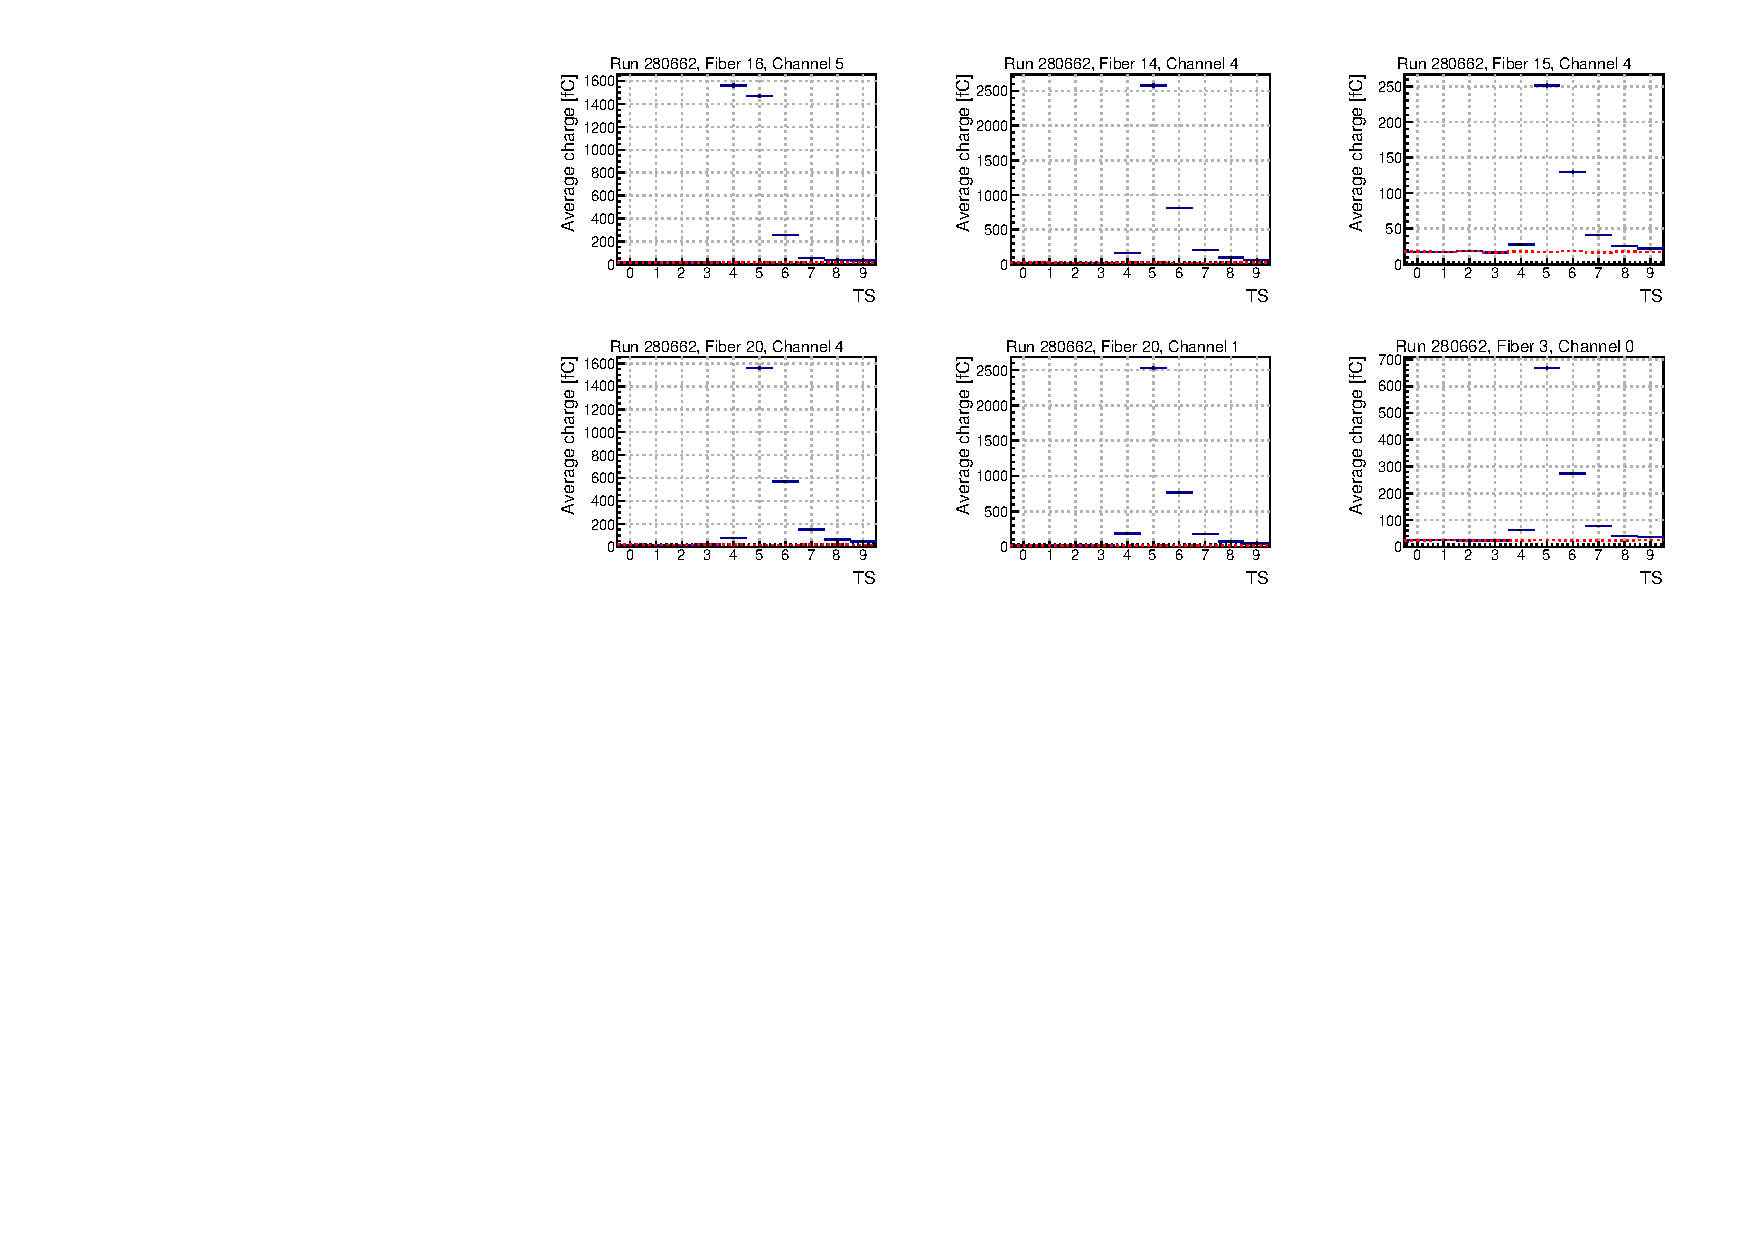
\includegraphics[width=0.97\textwidth]{figures/analysis/Pulse_shape_run280662_bright_SCSN81S.pdf}
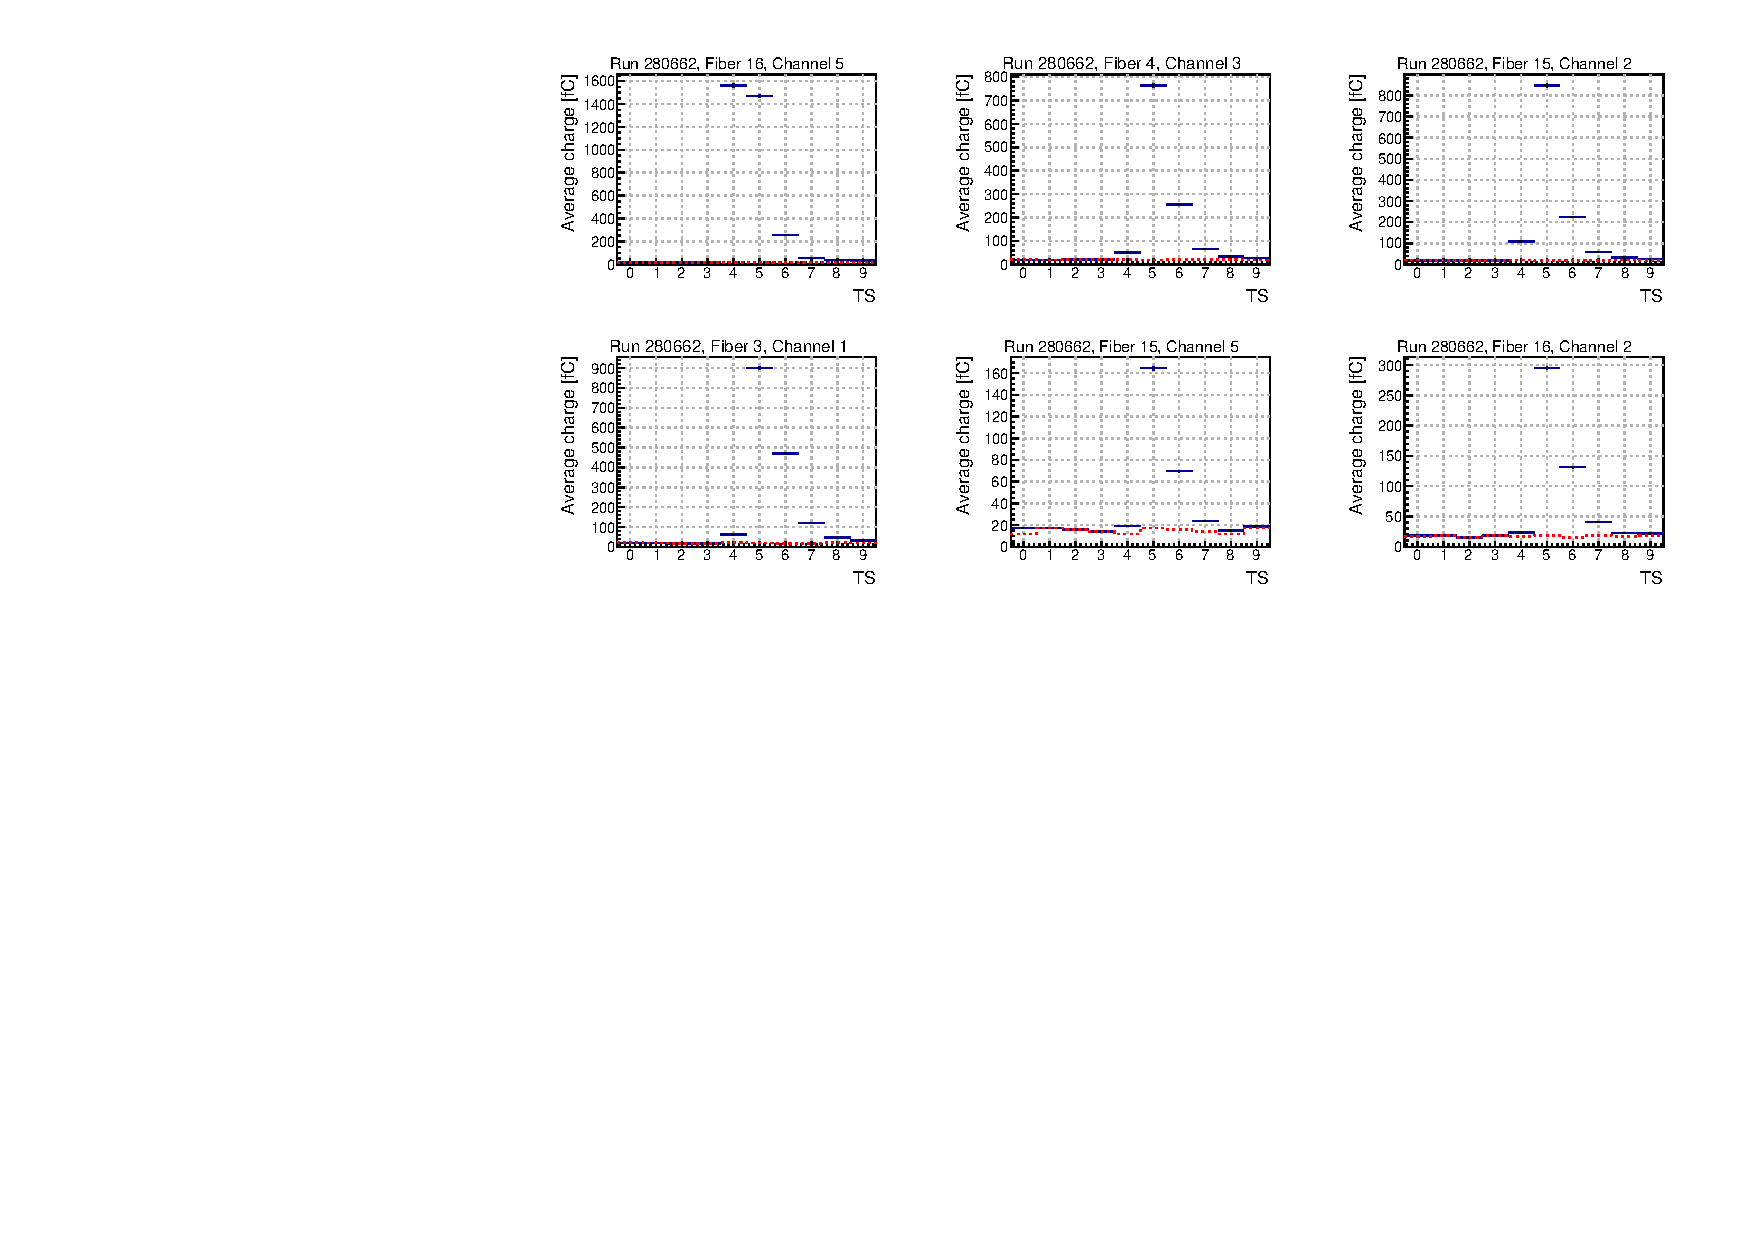
\includegraphics[width=0.97\textwidth]{figures/analysis/Pulse_shape_run280662_bright_others.pdf}
\caption{Average pulse shapes in response to laser (blue) and corresponding pedestals (red) at the time of installation for a selection of SCSN81-S channels (top half) and other materials (bottom half).}
\label{pulse0ifb}
\end{figure} 

\begin{figure}[tbp!]
\centering
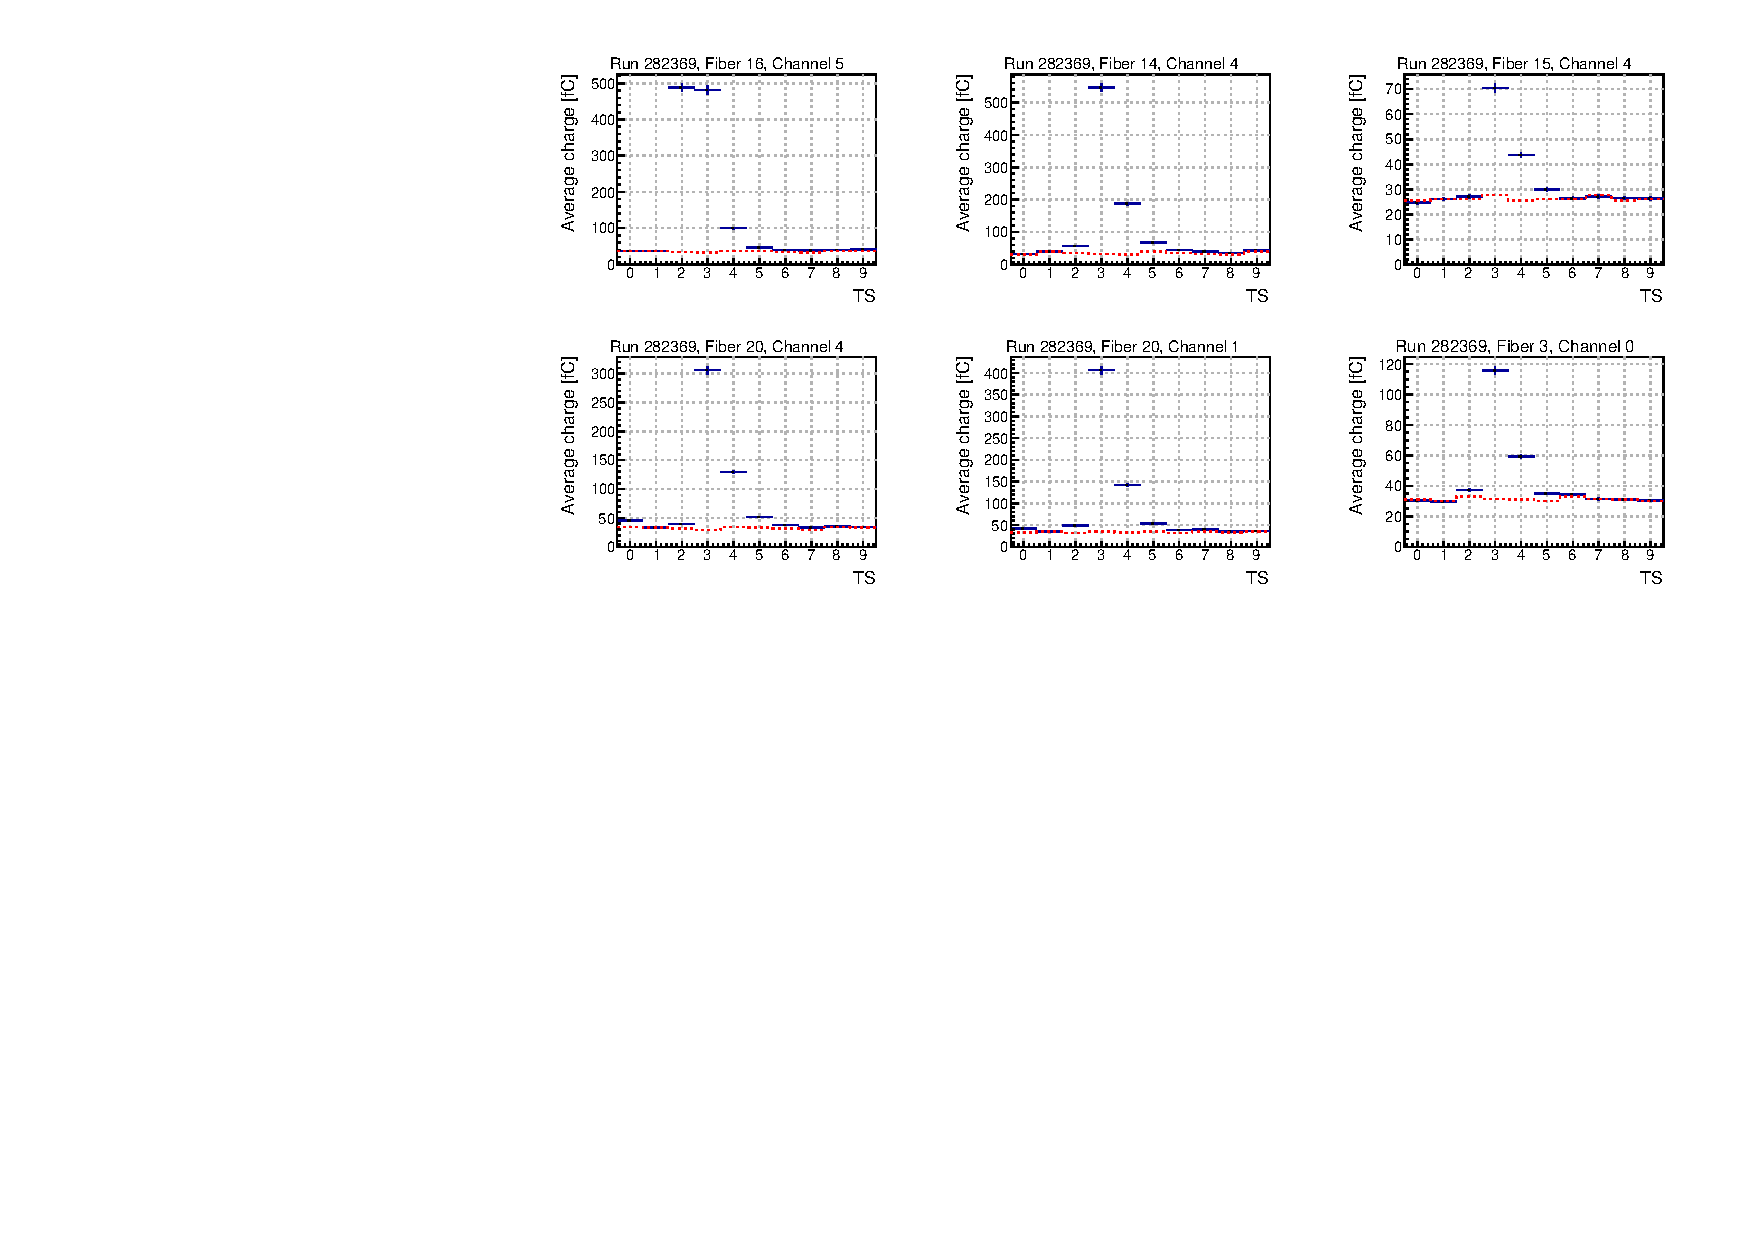
\includegraphics[width=0.97\textwidth]{figures/analysis/Pulse_shape_run282369_bright_SCSN81S.pdf}
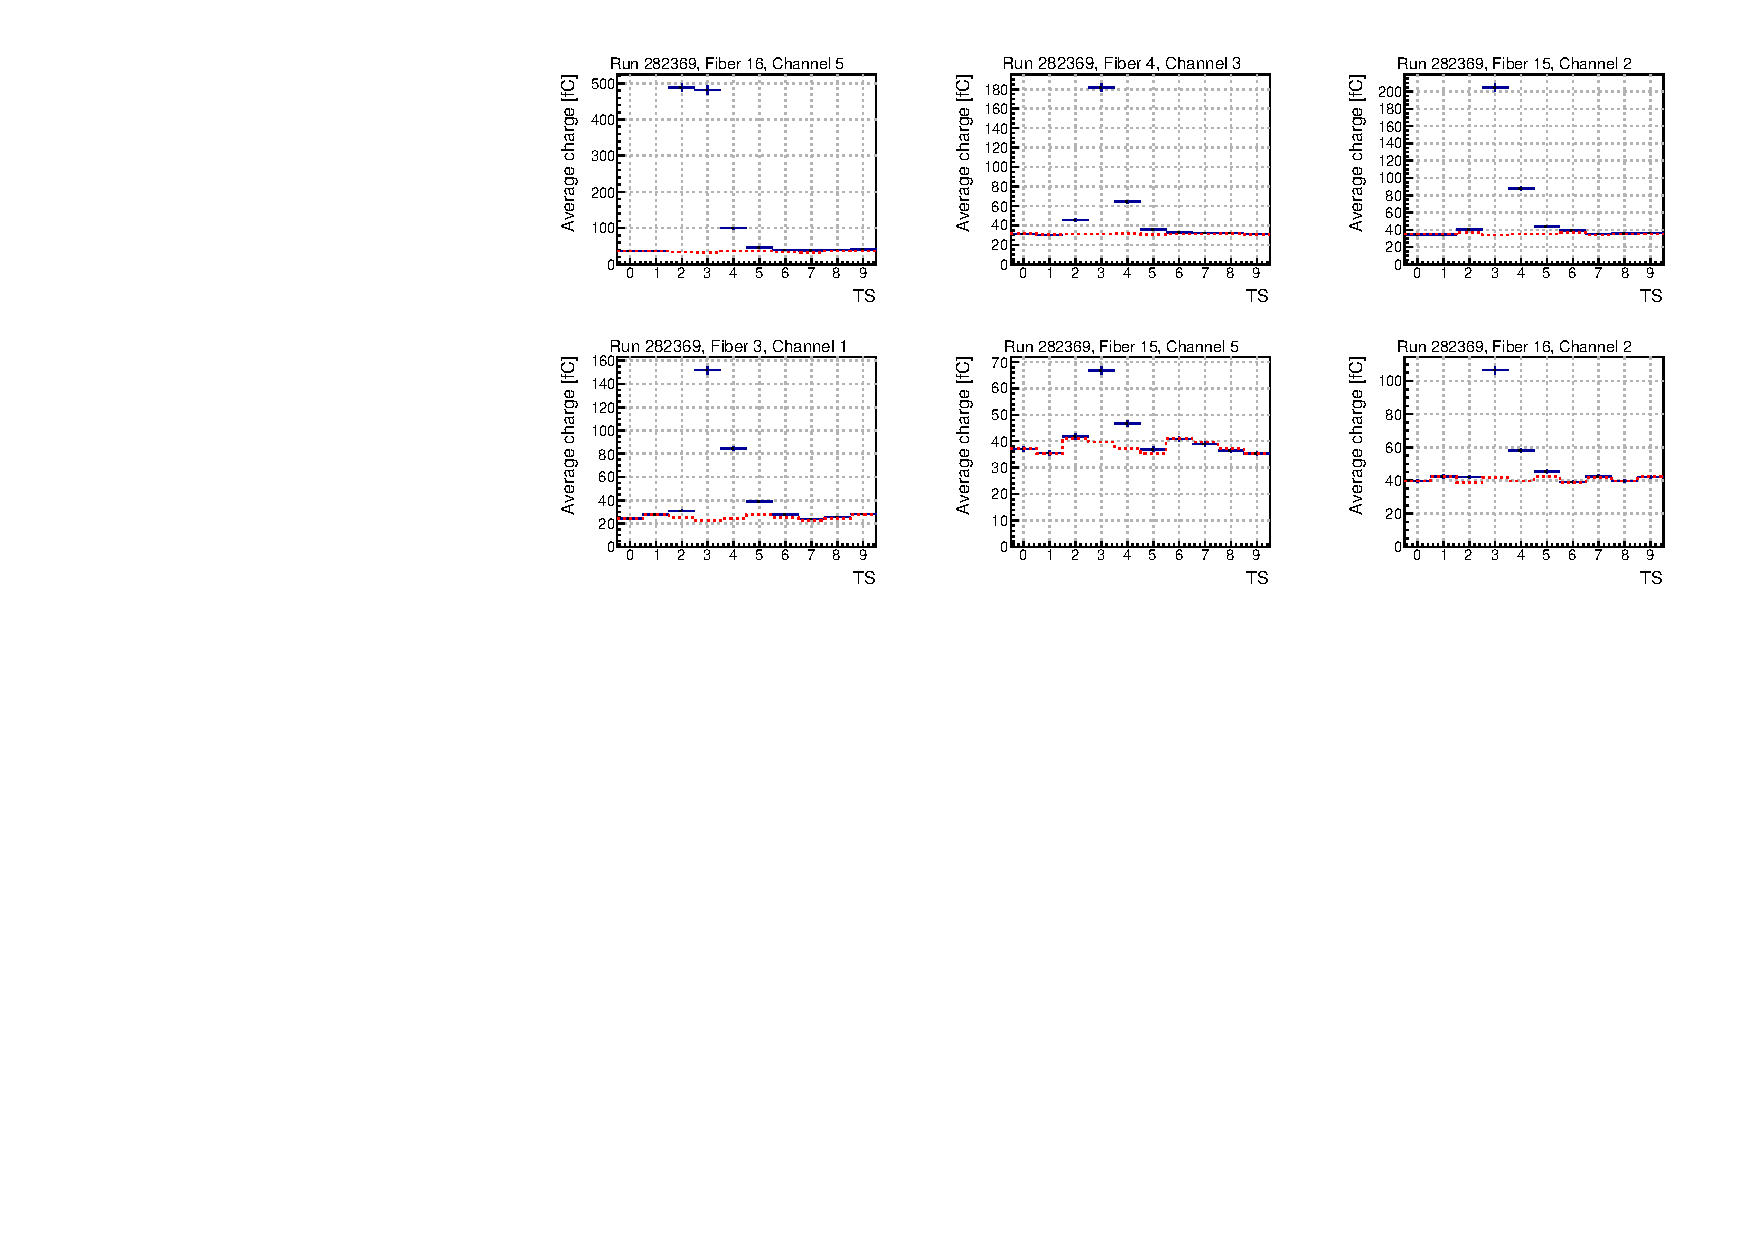
\includegraphics[width=0.97\textwidth]{figures/analysis/Pulse_shape_run282369_bright_others.pdf}
\caption{Average pulse shapes in response to laser (blue) and corresponding pedestals (red) after a delivered luminosity of 2.7 $\fbinv$ for a selection of SCSN81-S channels (top half) and other materials (bottom half).}
\label{pulse2p7ifb}
\end{figure} 

\begin{figure}[tbp!]
\centering
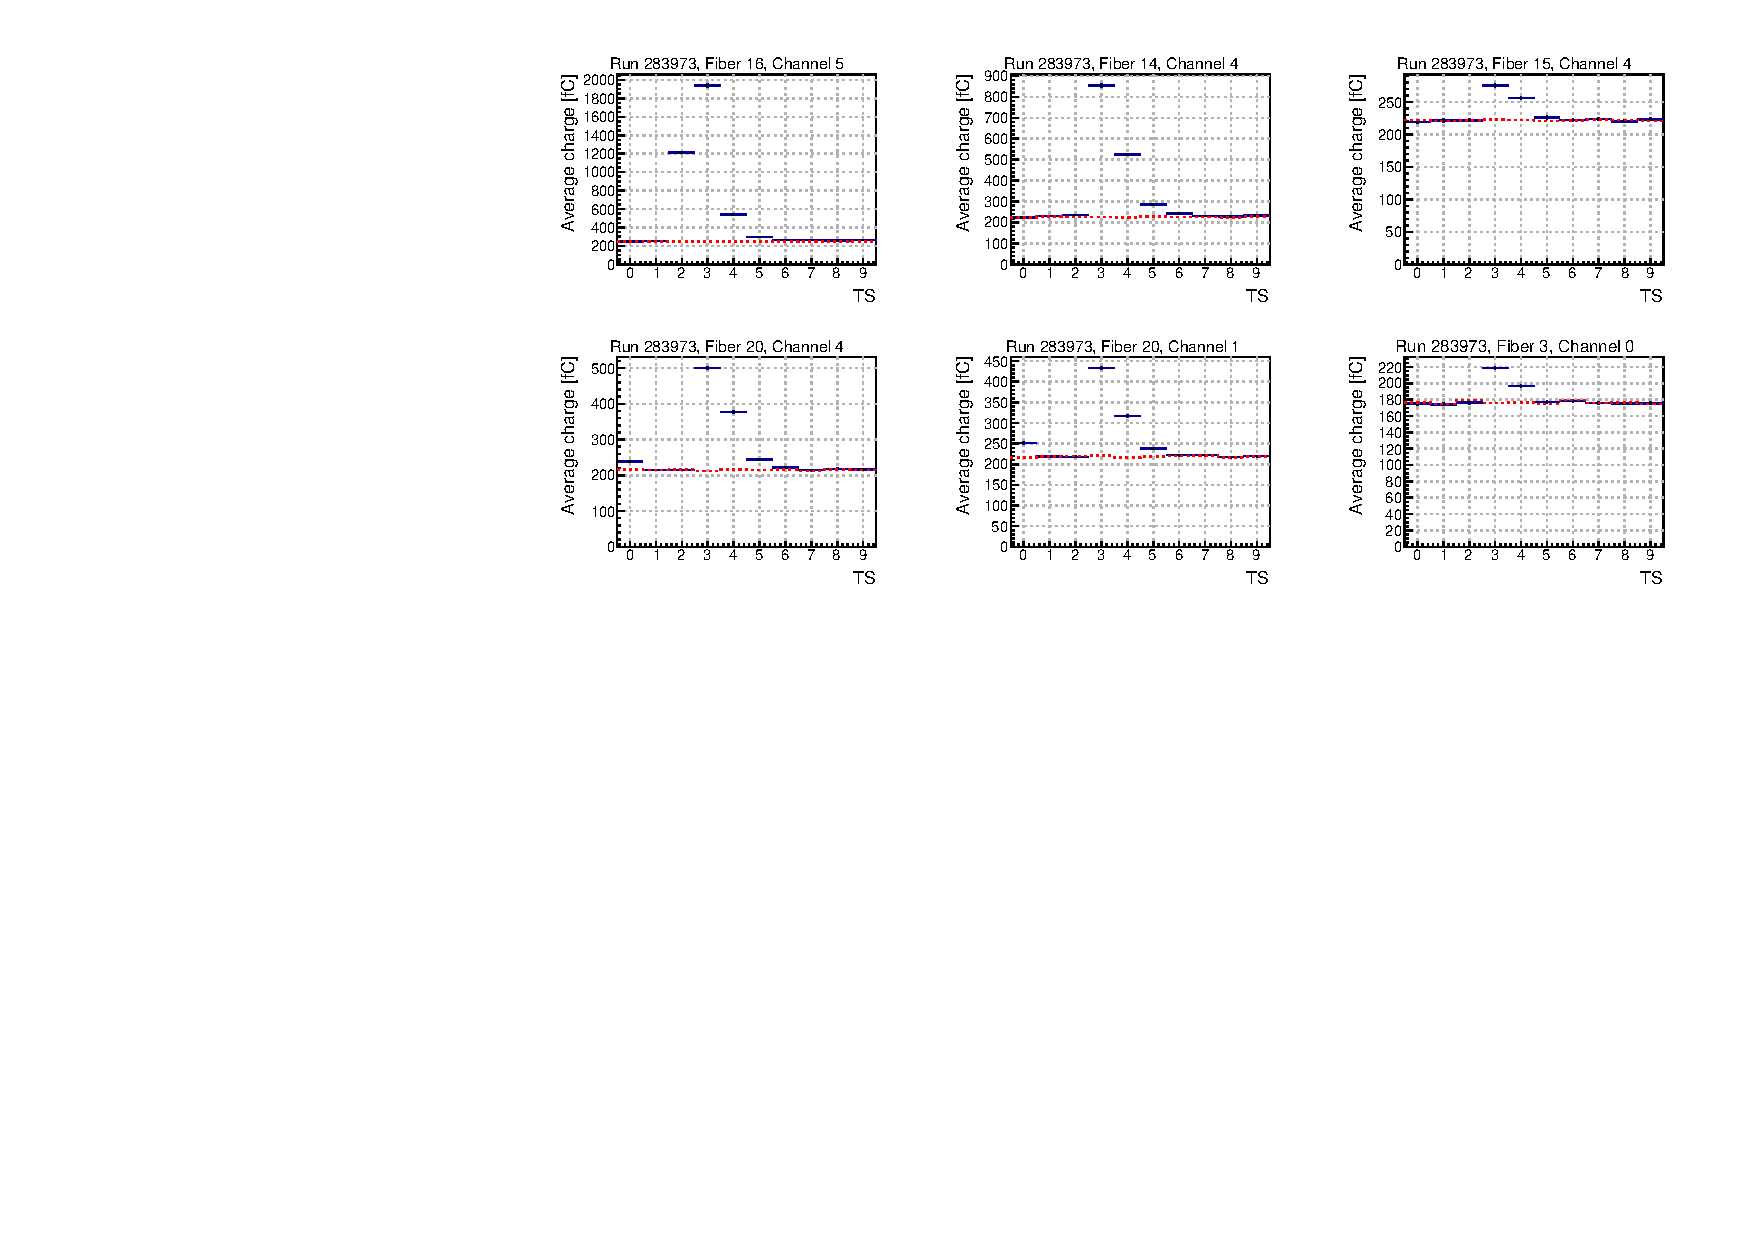
\includegraphics[width=0.97\textwidth]{figures/analysis/Pulse_shape_run283973_bright_SCSN81S.pdf}
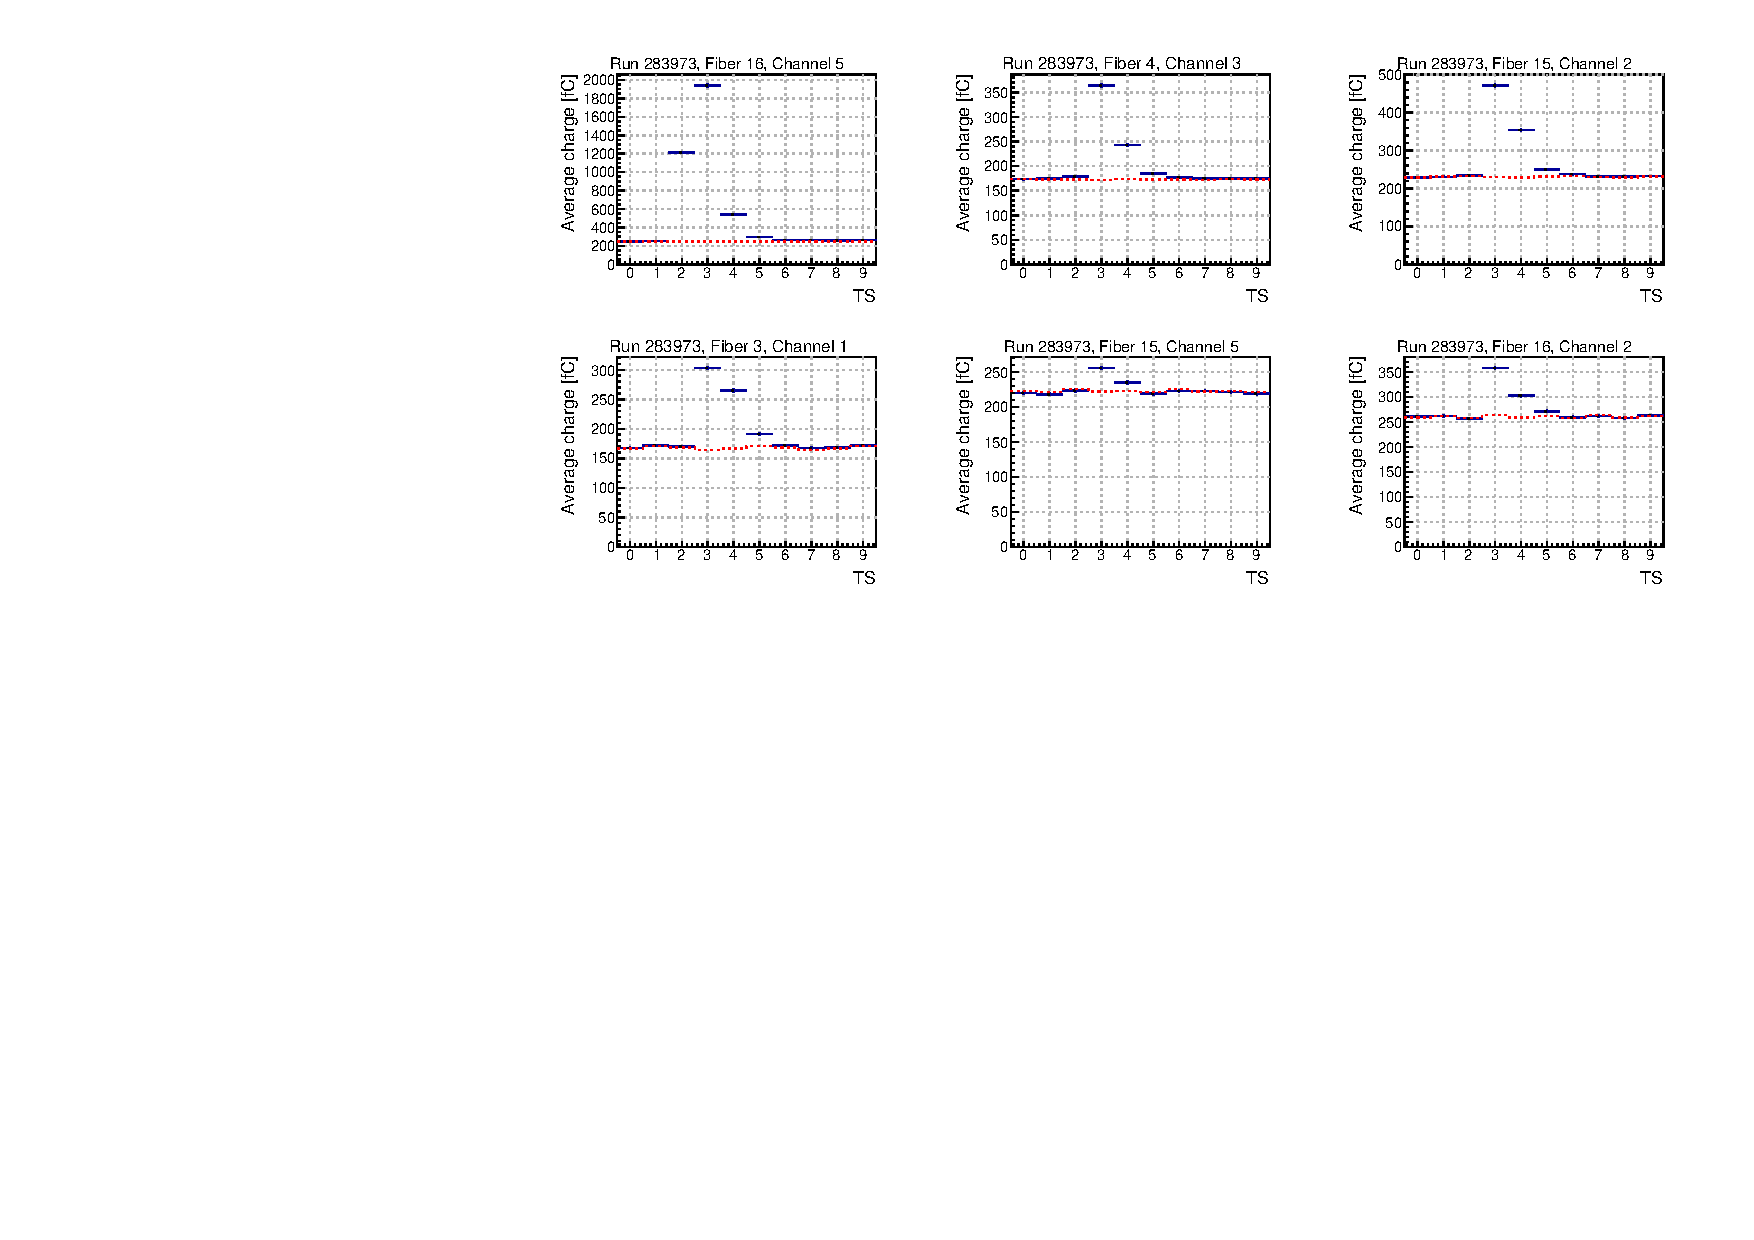
\includegraphics[width=0.97\textwidth]{figures/analysis/Pulse_shape_run283973_bright_others.pdf}
\caption{Average pulse shapes in response to laser (blue) and corresponding pedestals (red) after a delivered luminosity of 9.5 $\fbinv$ for a selection of SCSN81-S channels (top half) and other materials (bottom half).}
\label{pulse9p5ifb}
\end{figure} 

%\begin{figure}[tbp!]
%\centering
%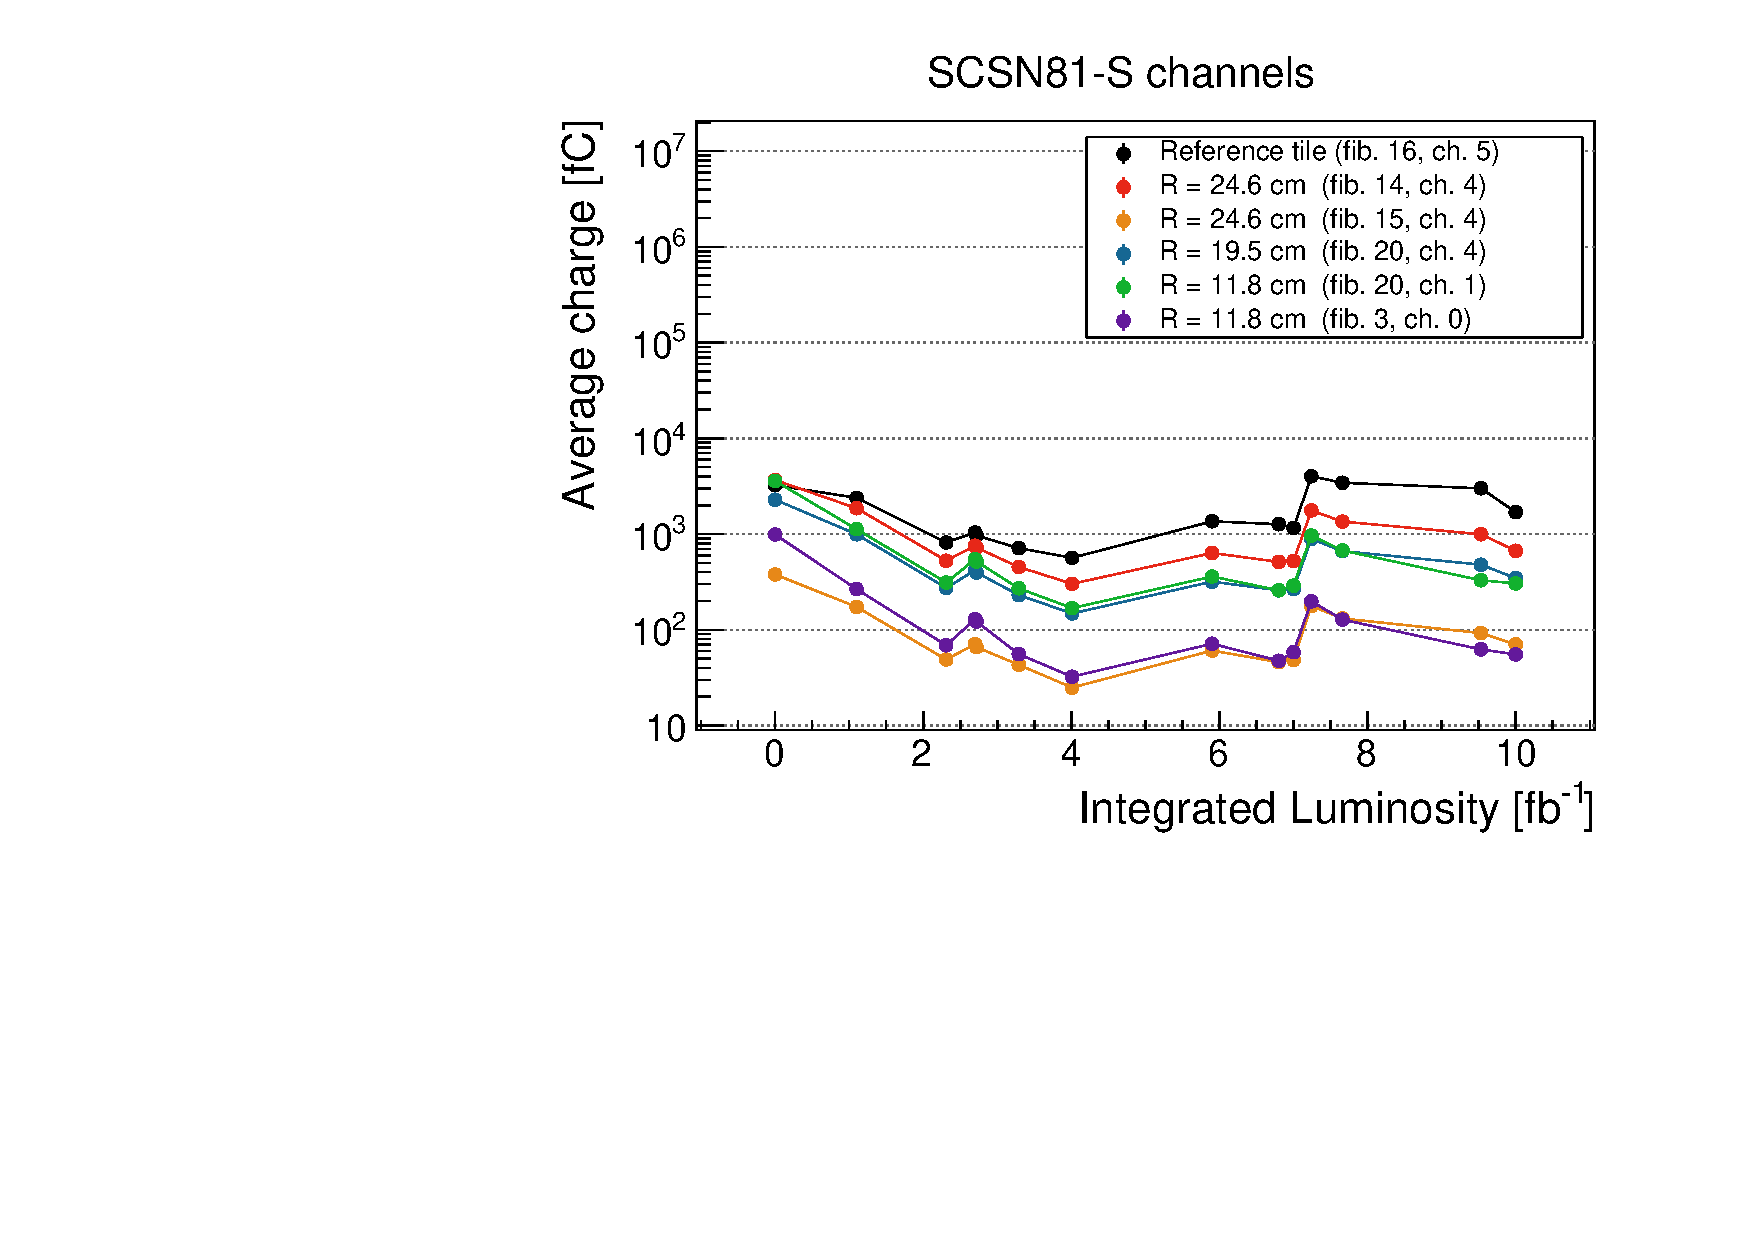
\includegraphics[width=0.46\textwidth]{figures/analysis/log_energy_lasercons_v14__scsnvar_vs_lumi.pdf}
%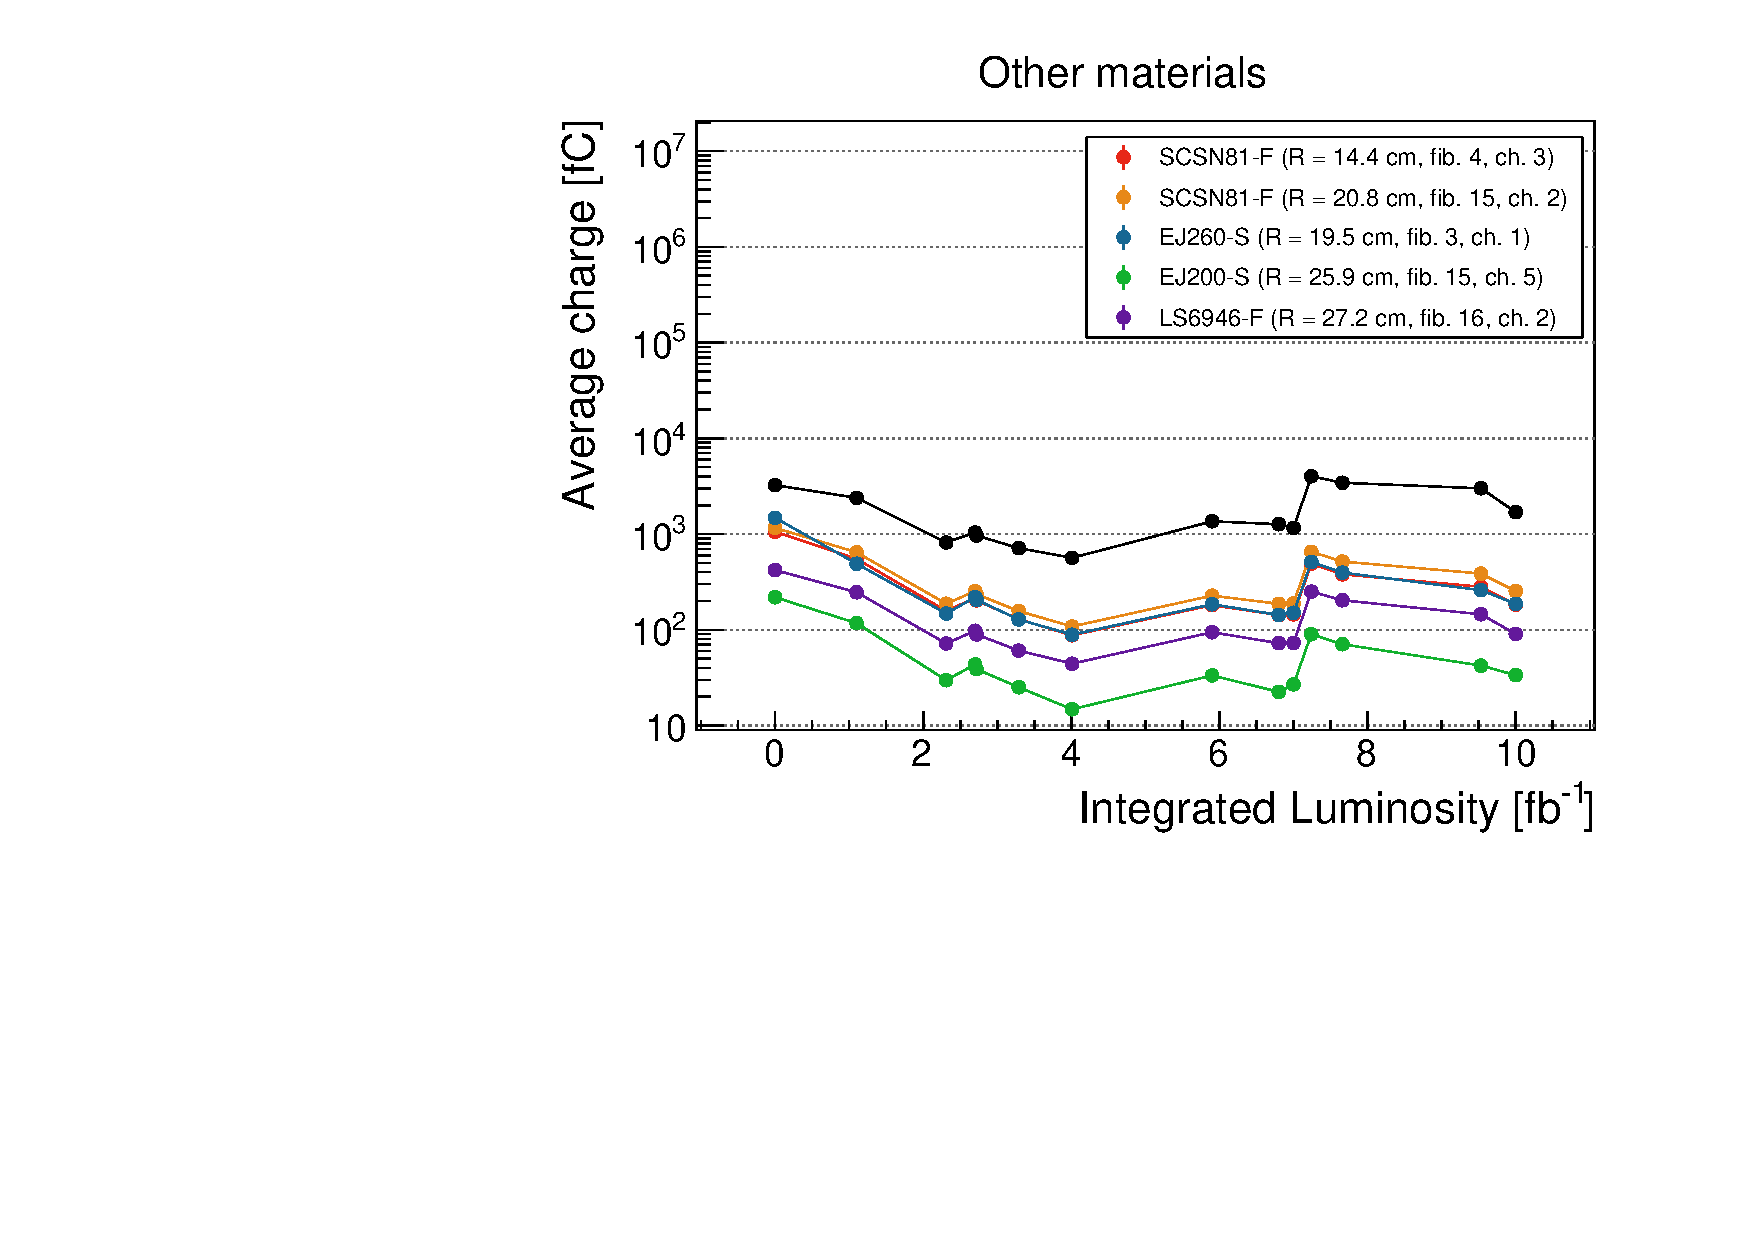
\includegraphics[width=0.46\textwidth]{figures/analysis/log_energy_lasercons_v14__bright_variety_vs_lumi.pdf}
%\caption{Progression of average laser response as a function of delivered luminosity, for a selection of channels. Left: SCSN81-S tiles. Right: variety of alternative tiles. Most variation in time is due to variation in laser amplitude.}
%\label{energy_raw}
%\end{figure}

%\begin{figure}[tbp!]
%\centering
%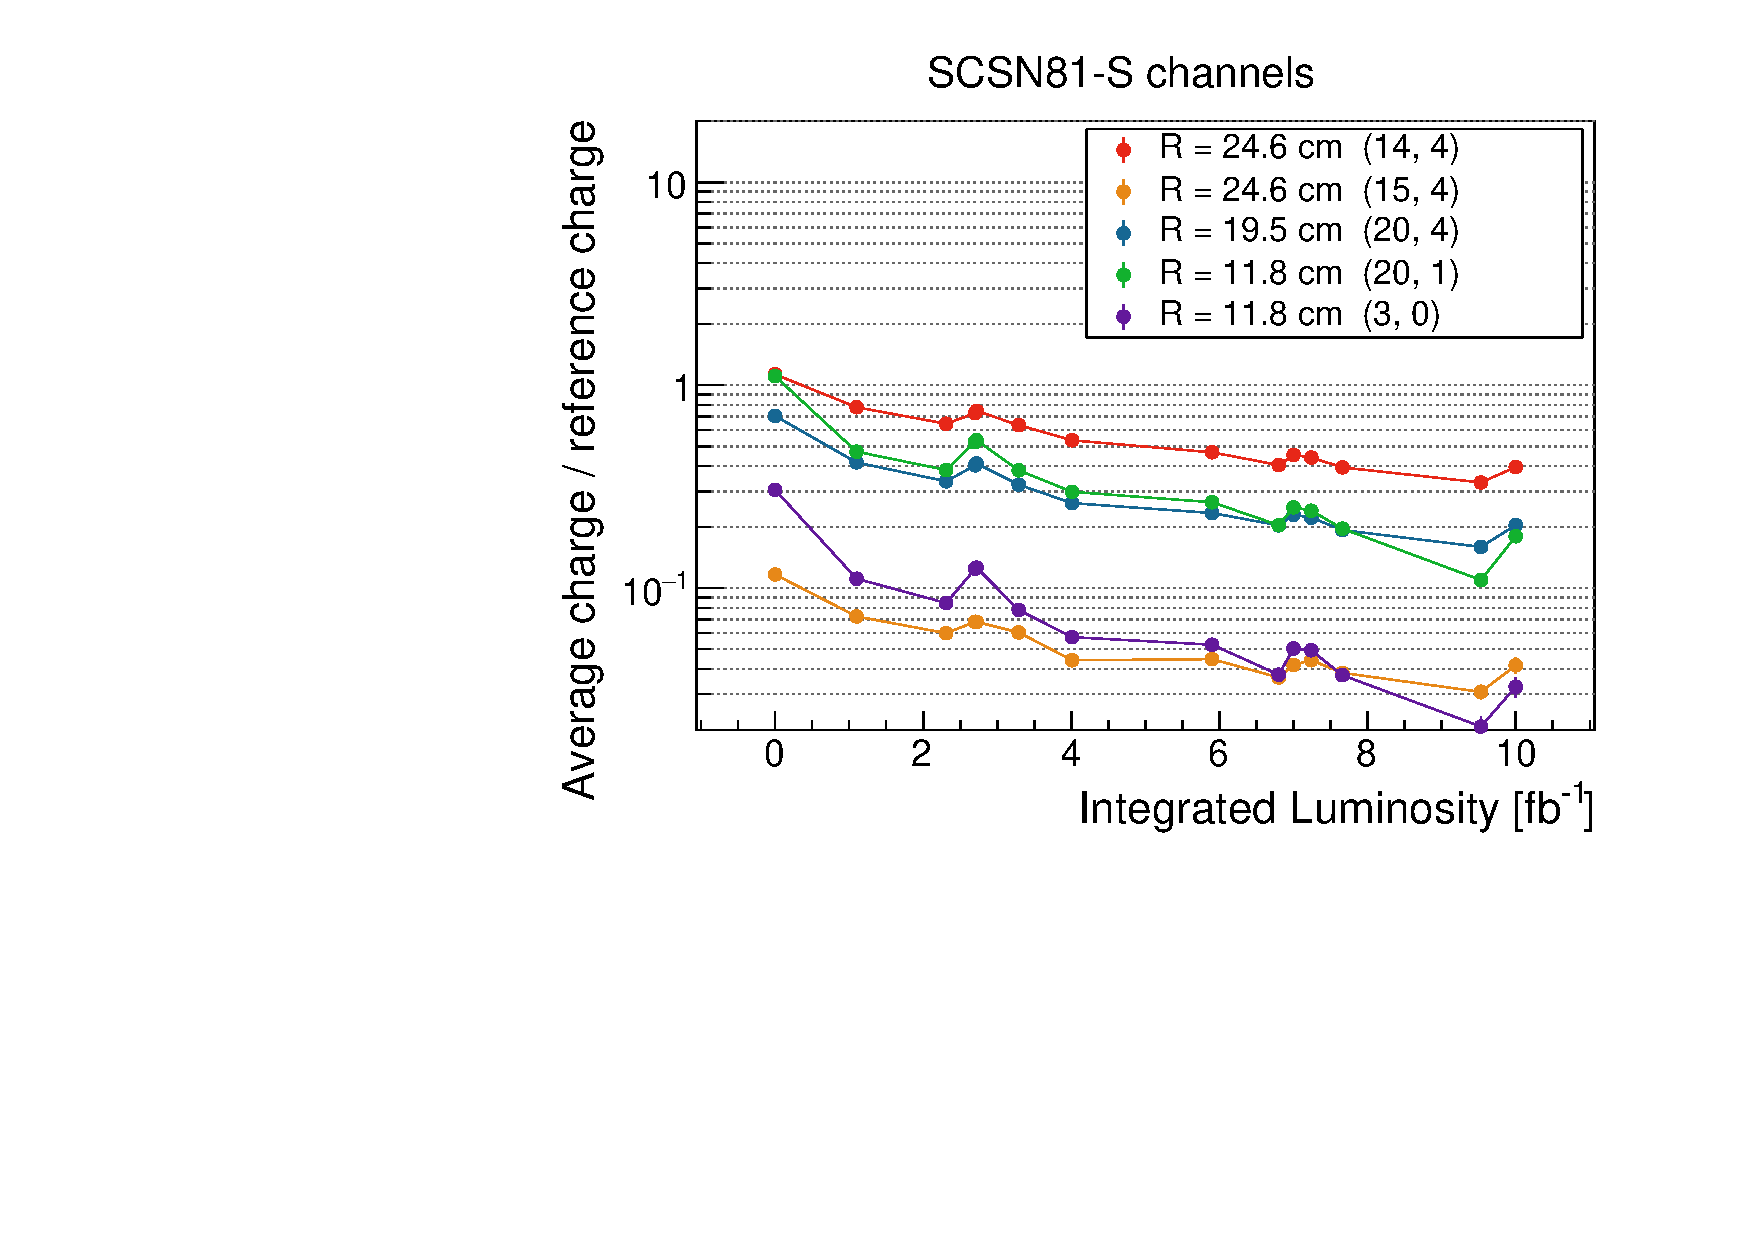
\includegraphics[width=0.46\textwidth]{figures/analysis/log_energy_lasercons_v14__scsnvar_vs_lumi_norm.pdf}
%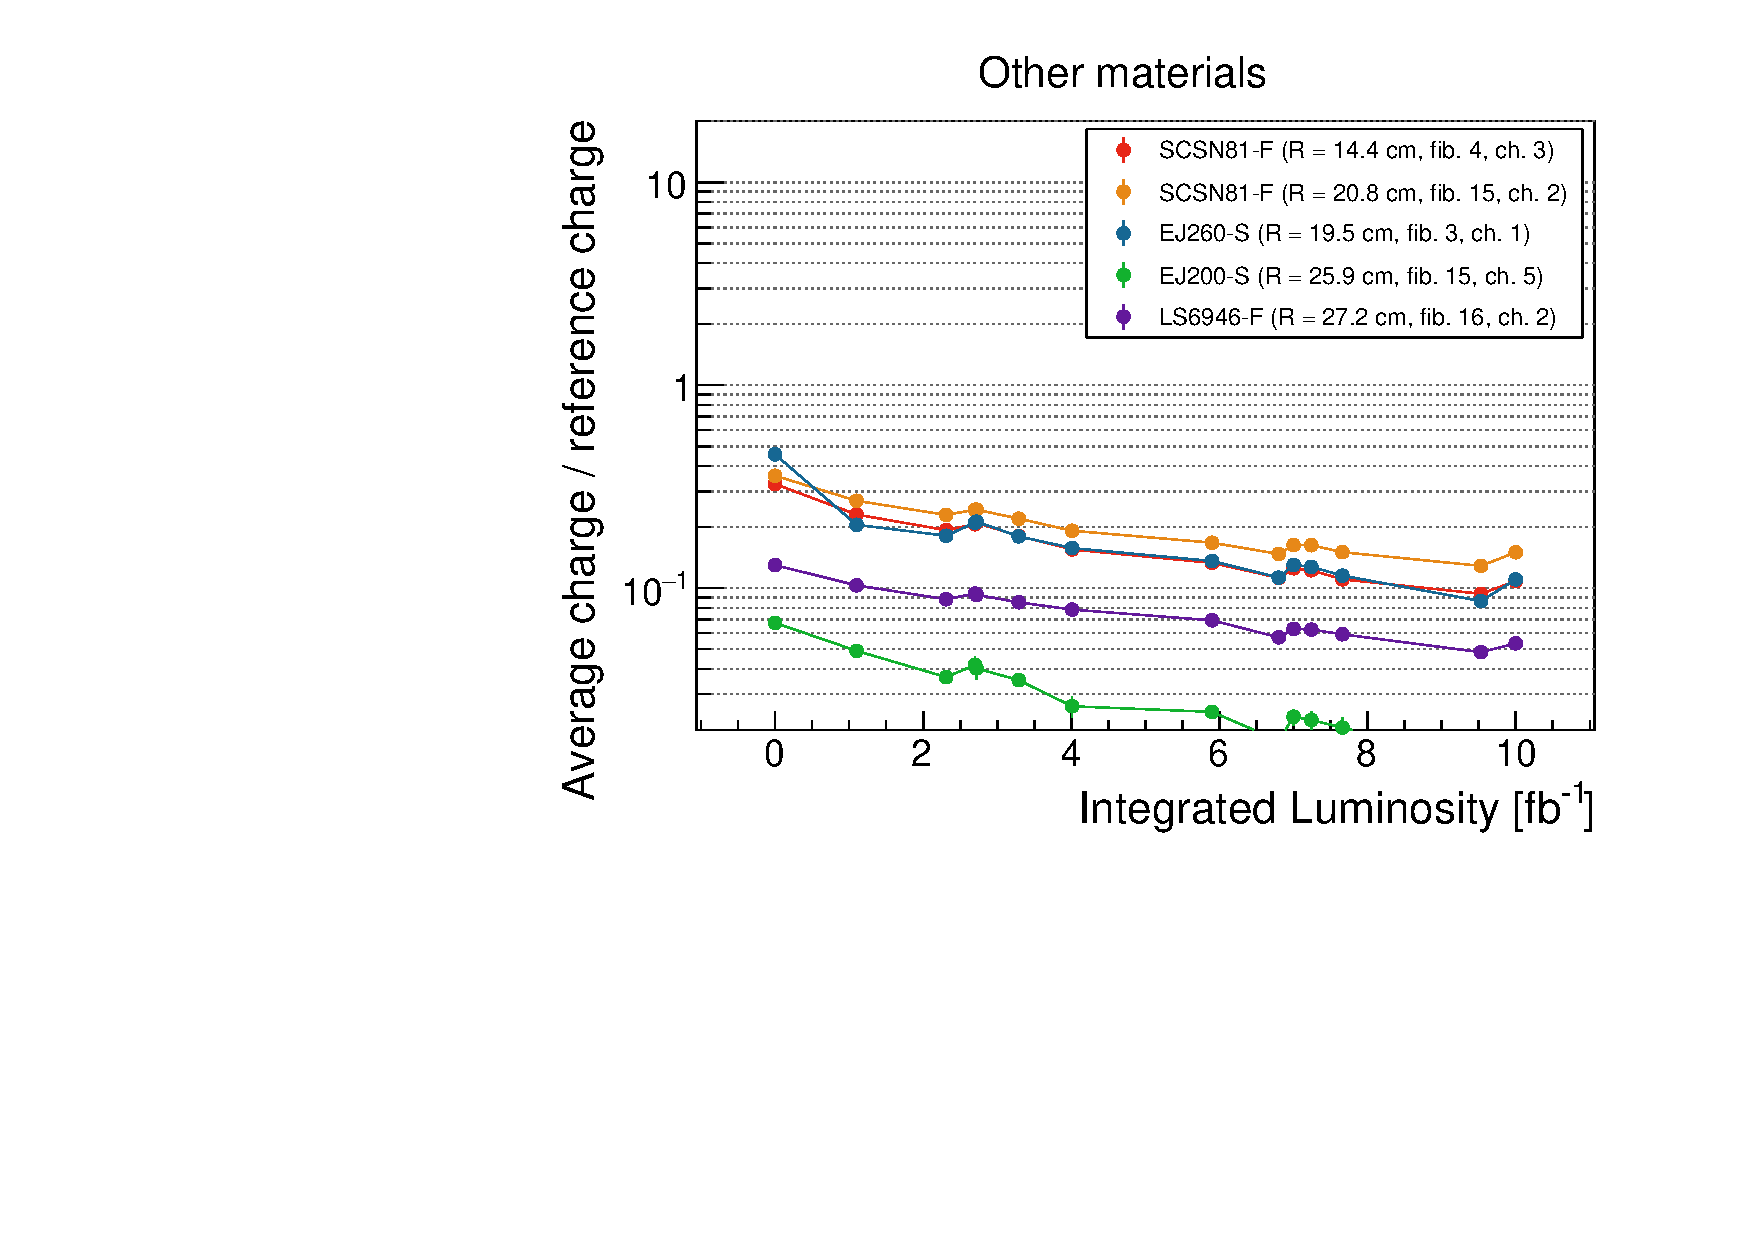
\includegraphics[width=0.46\textwidth]{figures/analysis/log_energy_lasercons_v14__bright_variety_vs_lumi_norm.pdf}
%\caption{Progression of average laser response normalized to the reference tile, as a function of delivered luminosity. Left: SCSN81-S tiles. Right: variety of alternative tiles. Variation due to laser amplitude is removed.}
%\label{energy_norm}
%\end{figure} 

%\begin{figure}[tbp!]
%\centering
%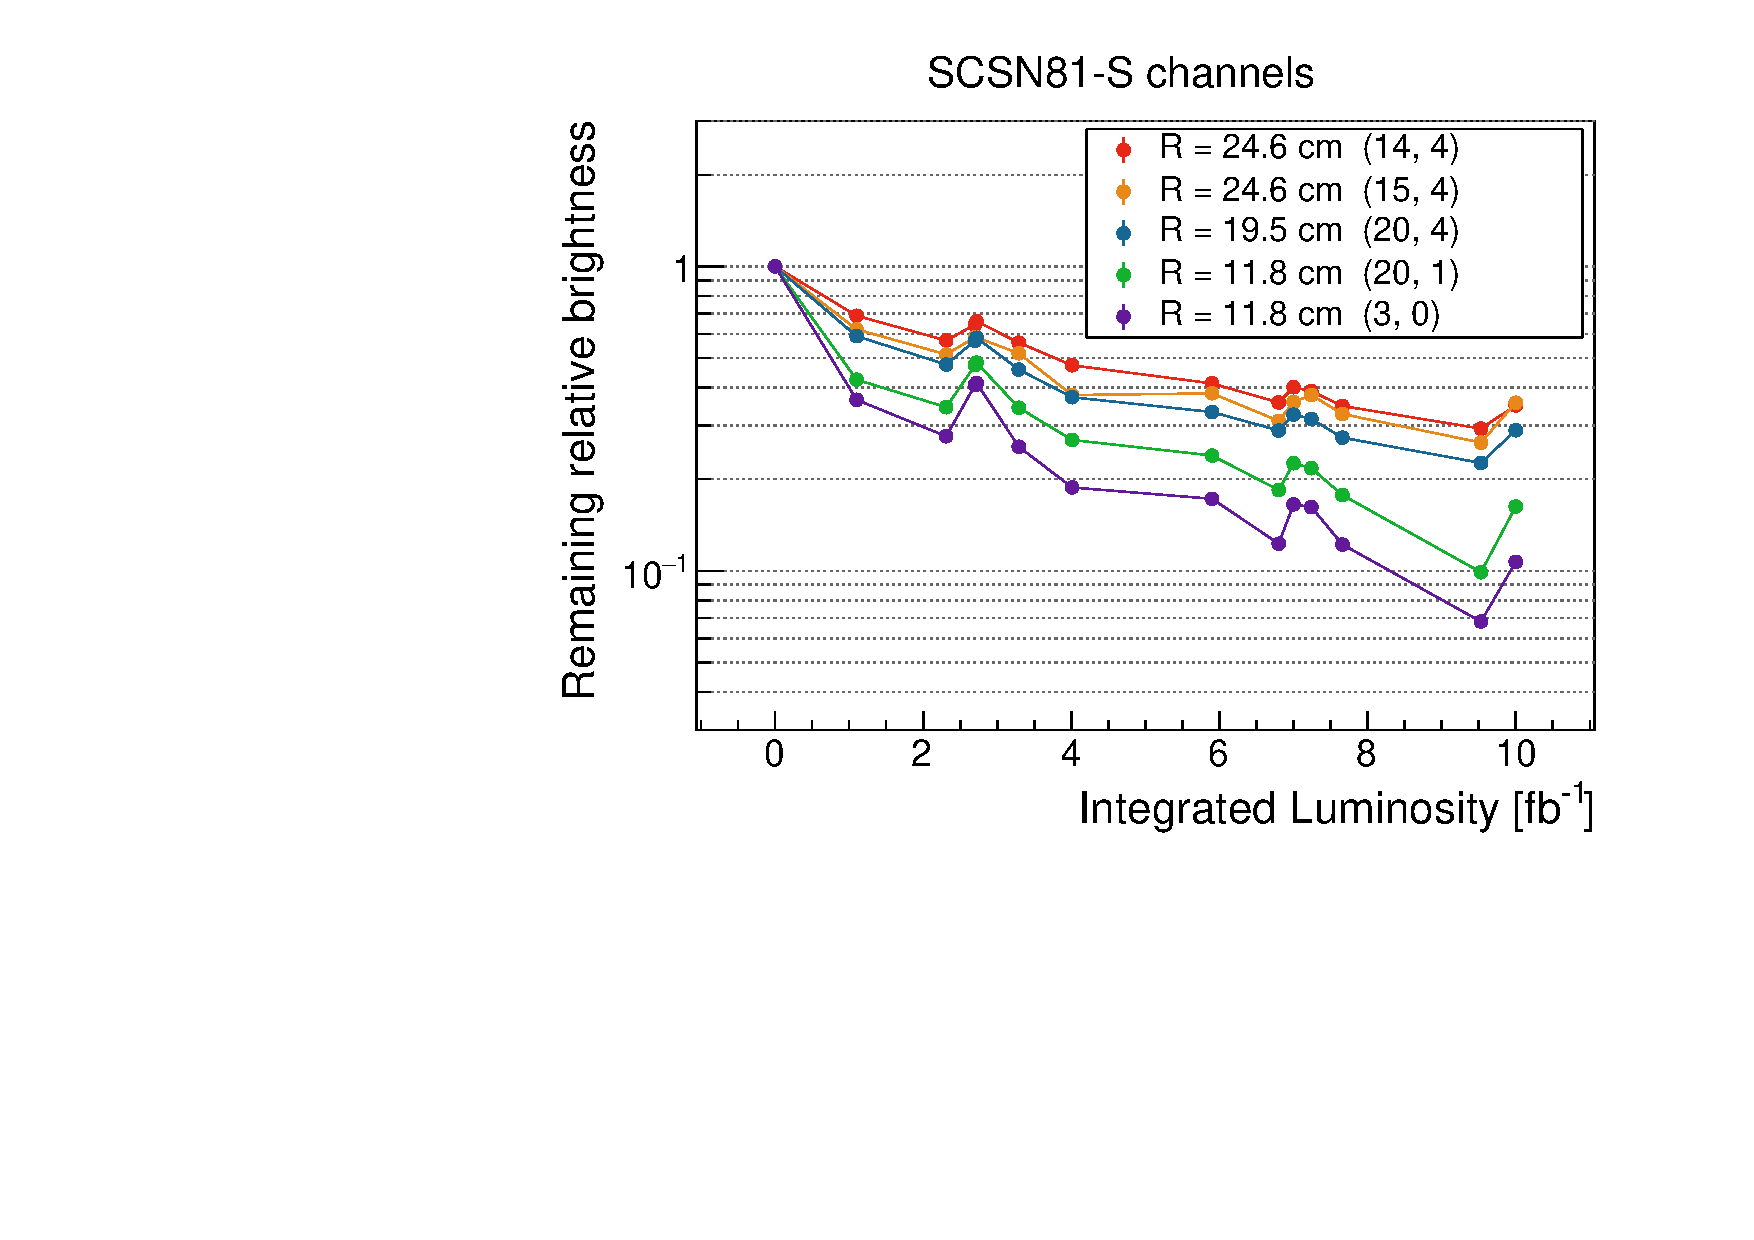
\includegraphics[width=0.46\textwidth]{figures/analysis/log_energy_lasercons_v14__scsnvar_vs_lumi_relative_change.pdf}
%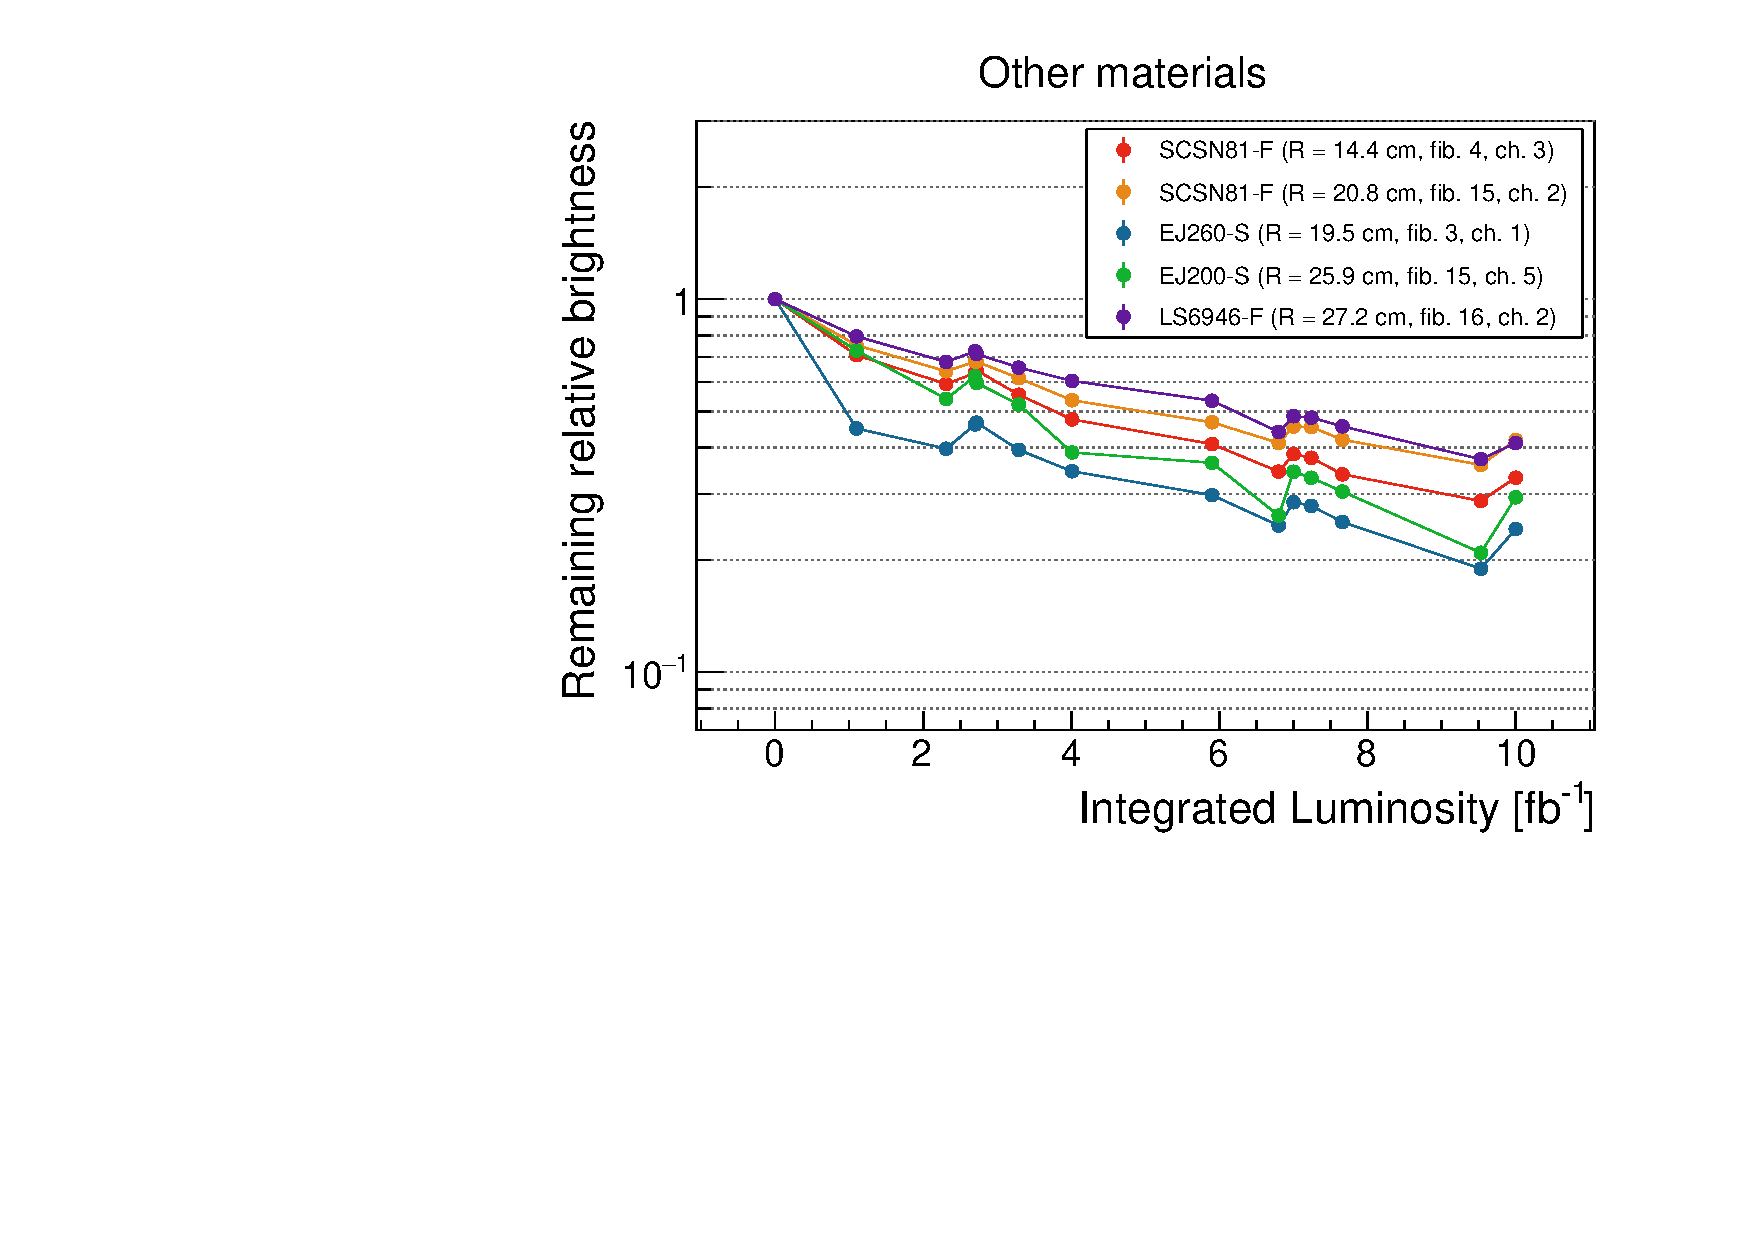
\includegraphics[width=0.46\textwidth]{figures/analysis/log_energy_lasercons_v14__bright_variety_vs_lumi_relative_change.pdf}
%\caption{Remaining laser response normalized to the initial response in each channel and to the reference tile response at each lumin%osity, as a function of delivered luminosity. Left: SCSN81-S tiles. Right: variety of alternative tiles.}
%\label{remaining_relative}
%\end{figure} 

%\begin{figure}[tbp!]
%\centering
%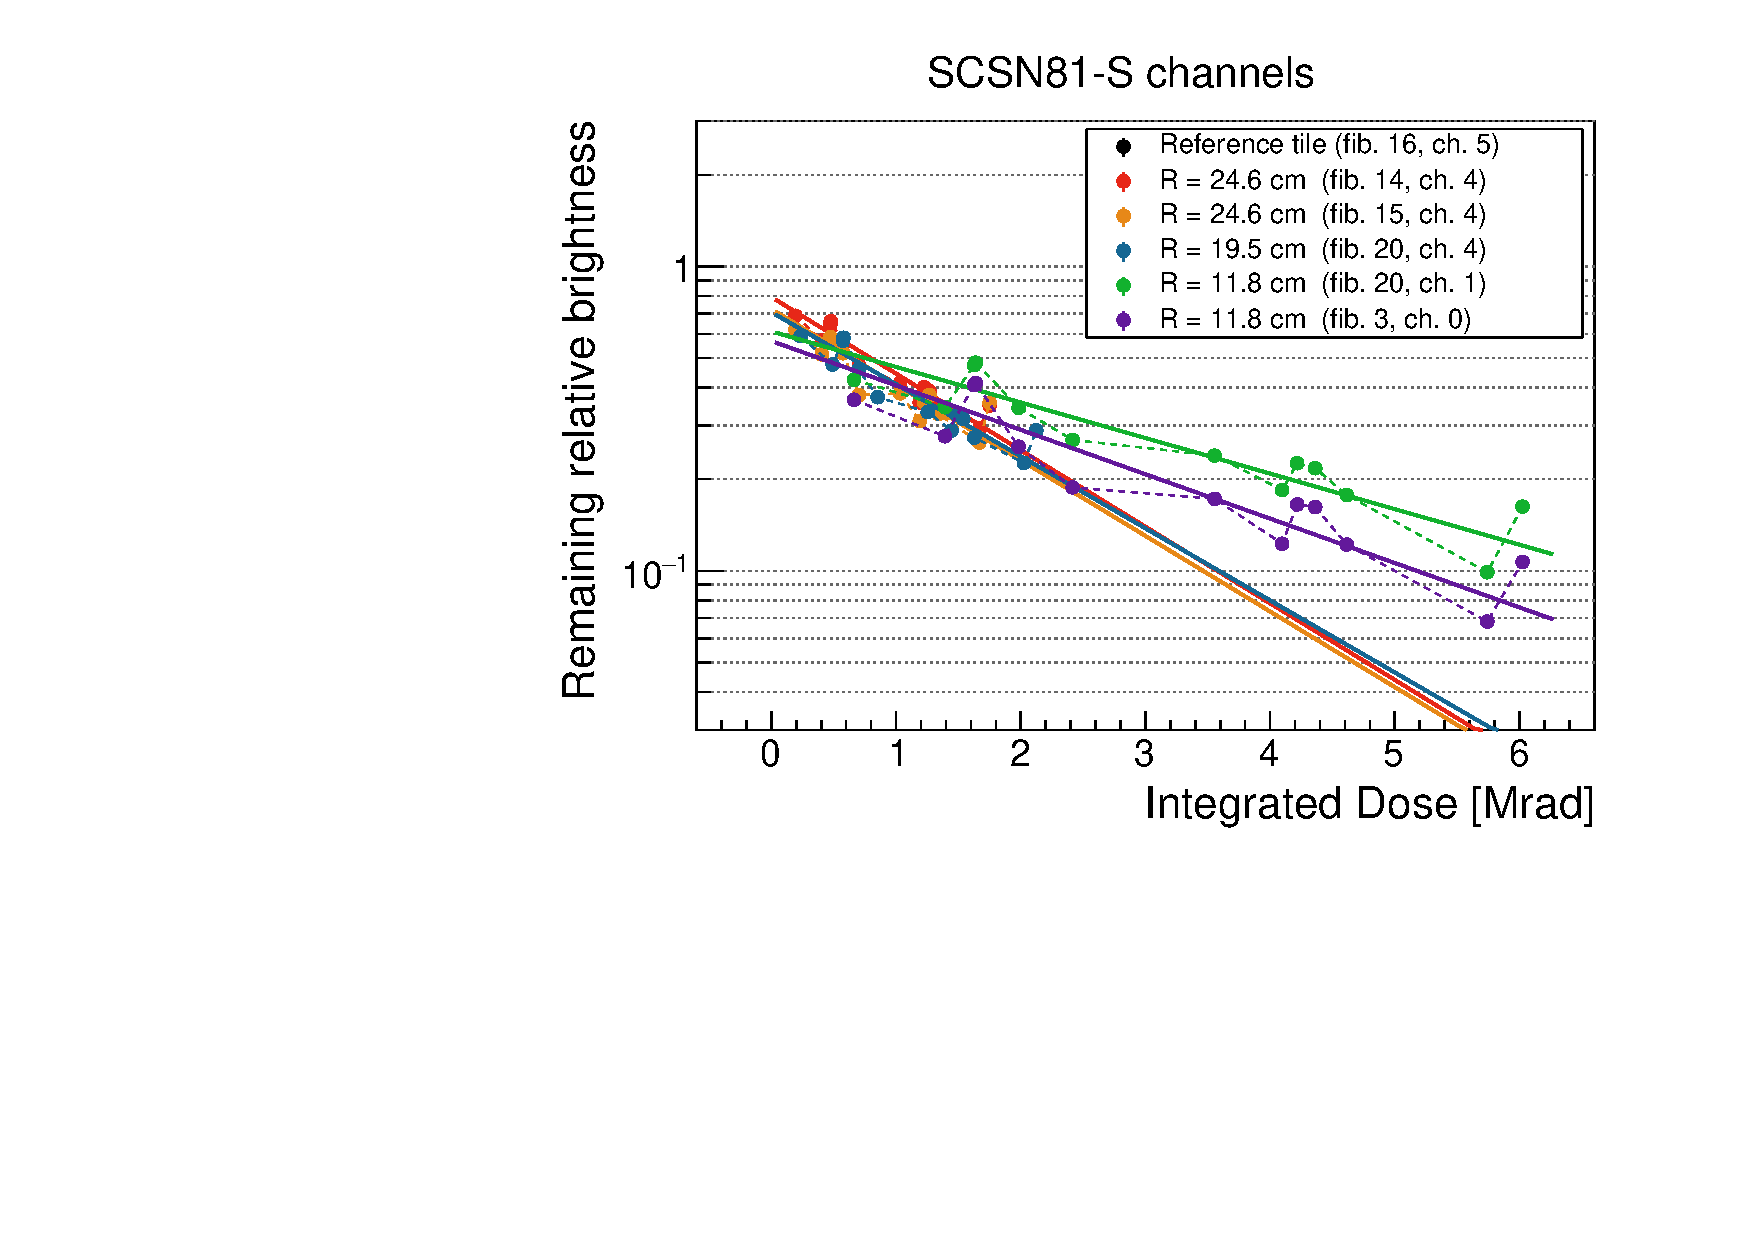
\includegraphics[width=0.46\textwidth]{figures/analysis/log_energy_lasercons_v14__scsnvar_vs_dose_relative_change.pdf}
%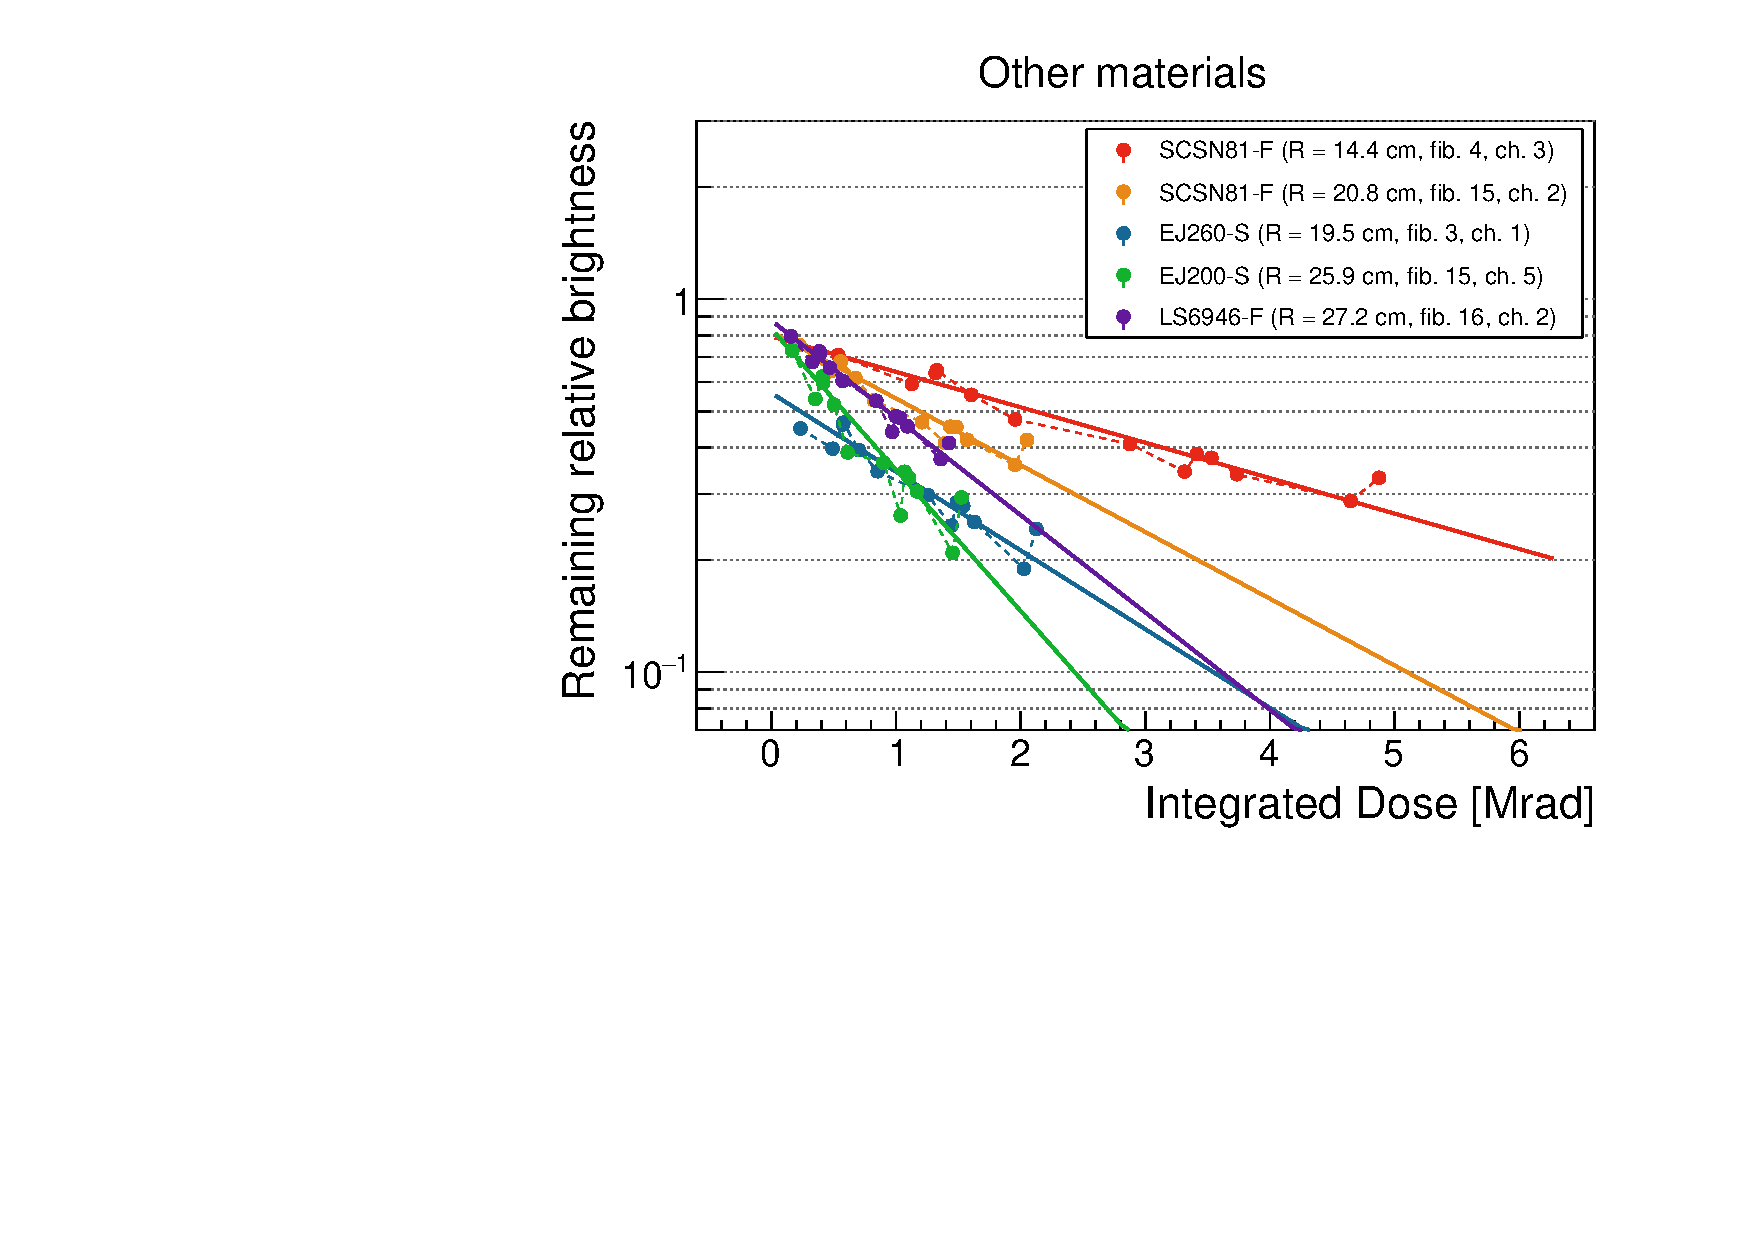
\includegraphics[width=0.46\textwidth]{figures/analysis/log_energy_lasercons_v14__bright_variety_vs_dose_relative_change.pdf}
%\caption{Remaining laser response as a function of received dose, normalized to the initial response in each channel and to the reference tile response at each measurement. Left: SCSN81-S tiles. Right: variety of alternative tiles. The slope of the remaining light yield indicates the dose constant. Shallower slopes (larger dose constants) are expected for tiles with greater irradiation due to dose rate effects.}
%\label{remaining_relative_dose}
%\end{figure} 


\subsection{Systematic uncertainties\label{sec:ana-unc}}

There are unknown and unmeasurable systematics at play in the experimental setup, including variation in the quality of the optical connection between laser and tiles after the laser splitting, unknown amounts of radiation damage to the reference tile used for normalization, and an unexplained steep drop in relative light yield for all tiles during the initial phase of irradiation, followed by a slower, steady-state exponential decay.

The light yield curve also shows a significant amount of recovery in the post-collisions period when there was no irradiation. The dose constants measured in this paper are measured after the temporary damage in the tiles has annealed and only the permanent damage remains. However, the day-0 light yield cannot be used as the pre-irradiation value for the steady-state exponential decay because the initial stage of the damage mechanism is characterized by the steeper rate of light loss that is not yet understood. Therefore, the L(0) value used in the calculation of the post-recovery dose constant is found by fitting an exponential curve to the L(\textit{d})/L(0) points as a function of integrated dose only during the steady-state exponential decay region, extrapolating the curve to a dose of 0 Mrad, and taking the dose = 0 intercept as L(0) in Equation~\ref{eq:lightloss}. The equation is then solved for the dose constant D.

The statistical uncertainty on each L(\textit{d})/L(0) measurement is calculated via error propagation from the RMS's of the light yield distributions of the signal and reference tiles at dose \textit{d} and on day 0.

All in all, the light yield curve exhibits variations larger than the statistical uncertainty, due to an ensemble of systematics including the steep drop in the initial state of irradiation and also run-to-run variation in light transmission from tile to readout module. To cover this, a conservative systematic uncertainty of 20\% is added in quadrature to the statistical uncertainty to yield the total uncertainty.

\subsection{Results\label{sec:ana-res}}

\subsubsection{Light yield versus dose\label{sec:ana-res-lyvsdose}}

The relative light yields for the various tiles as a function of total received dose are shown here in Figures~\ref{fig:SCSN81-S-11p8cm-dose} to~\ref{fig:EJ260-F-dose}. Each plot shows also the fitted exponential curve to the steady-state exponential decay, which is used to extrapolate to zero dose to get the initial light yield used to solve for the dose constant after recovery.

\begin{figure}[tbp!]
\centering
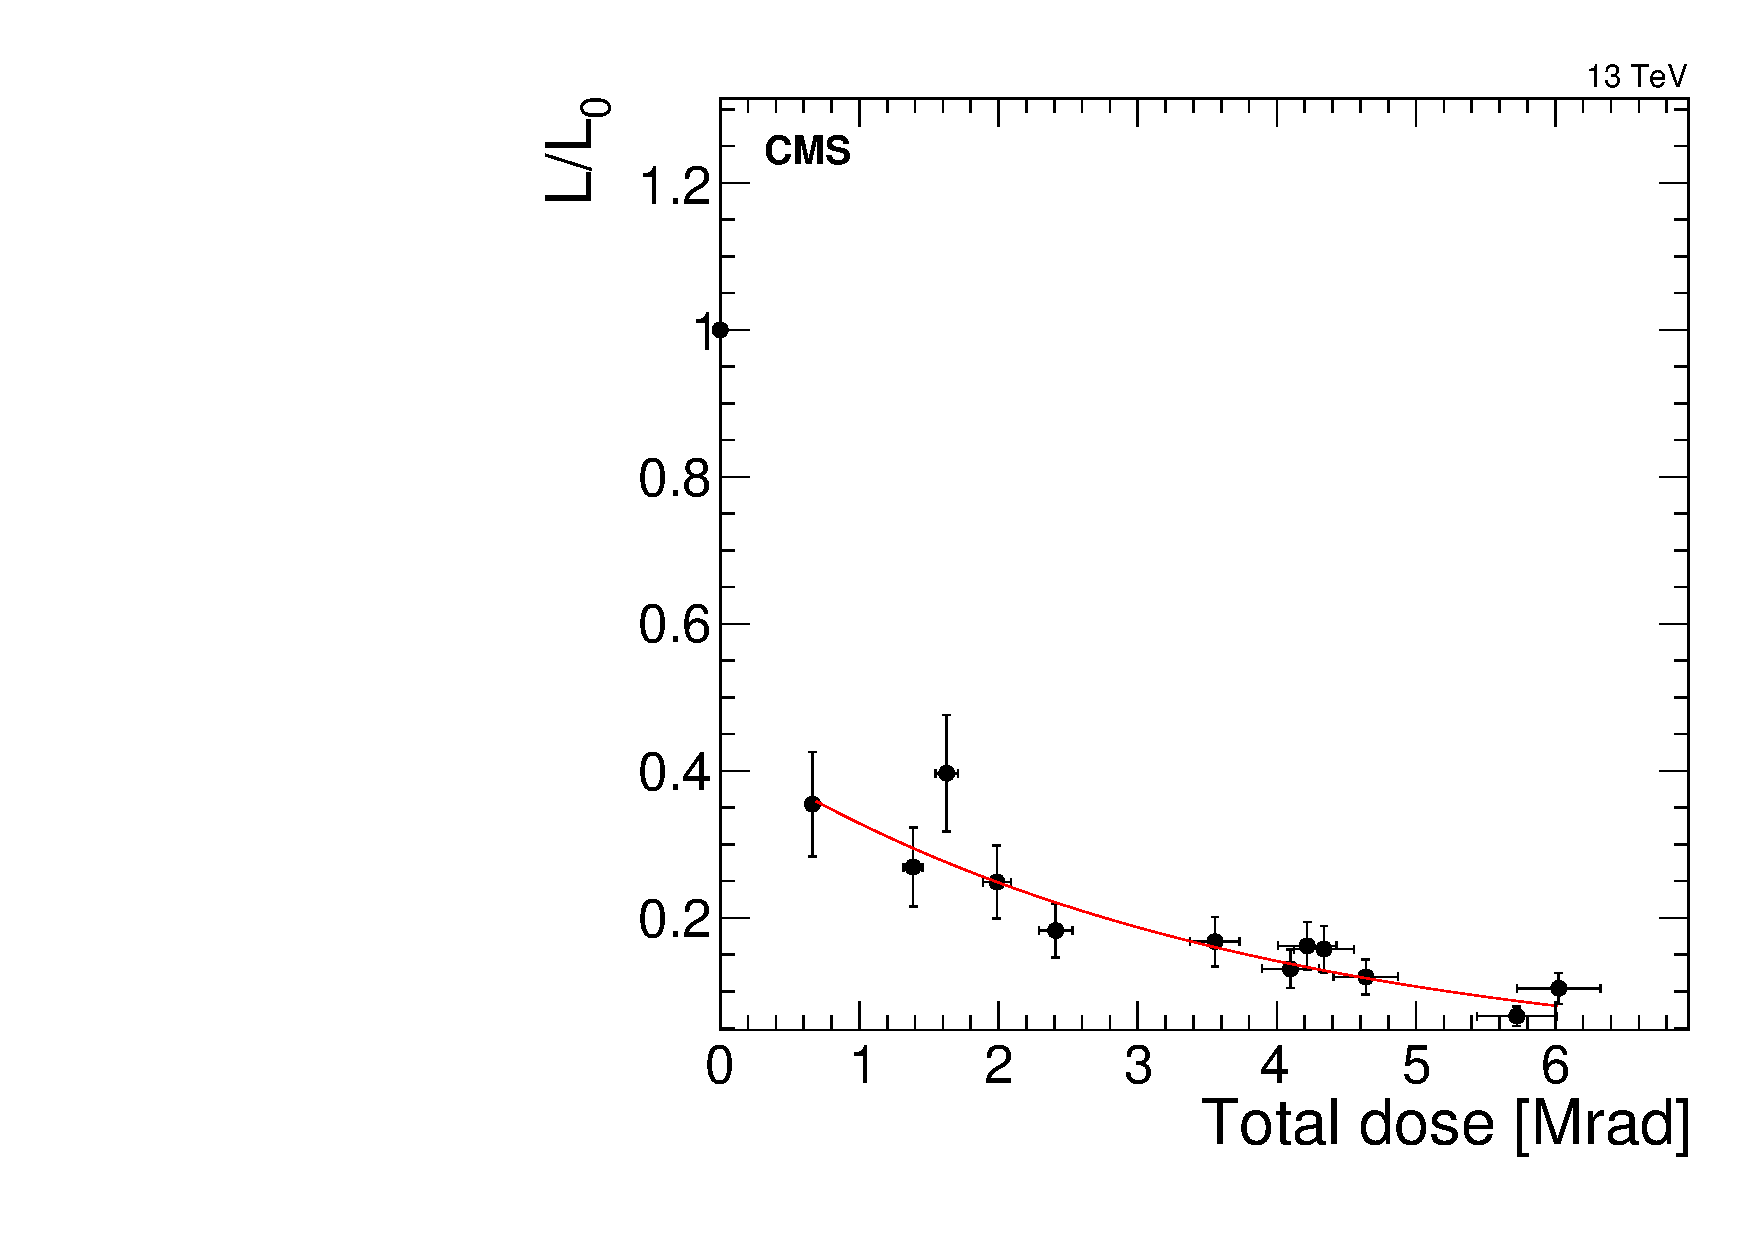
\includegraphics[width=0.45\textwidth]{figures/SCSN81-S-11p8cm-f3ch0-dose.pdf}
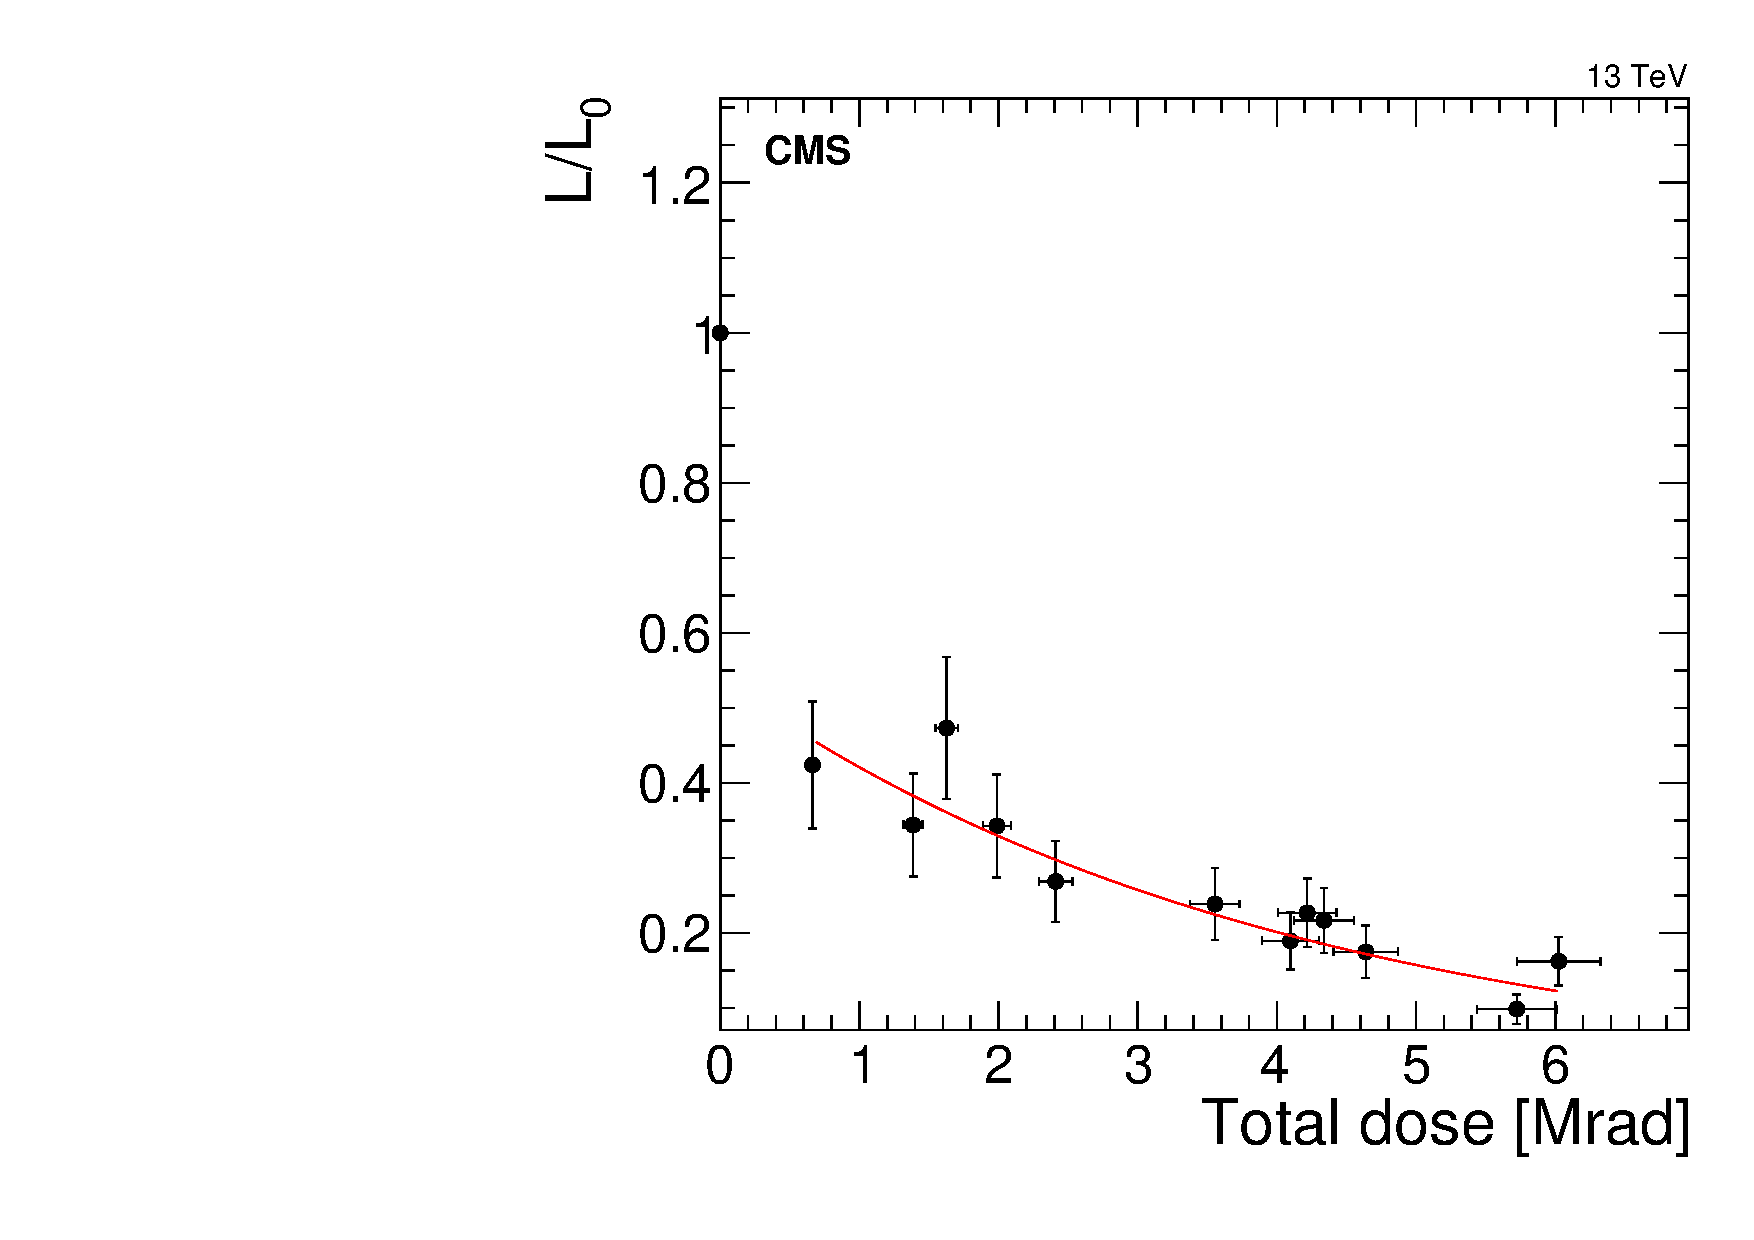
\includegraphics[width=0.45\textwidth]{figures/SCSN81-S-11p8cm-f20ch1-dose.pdf}
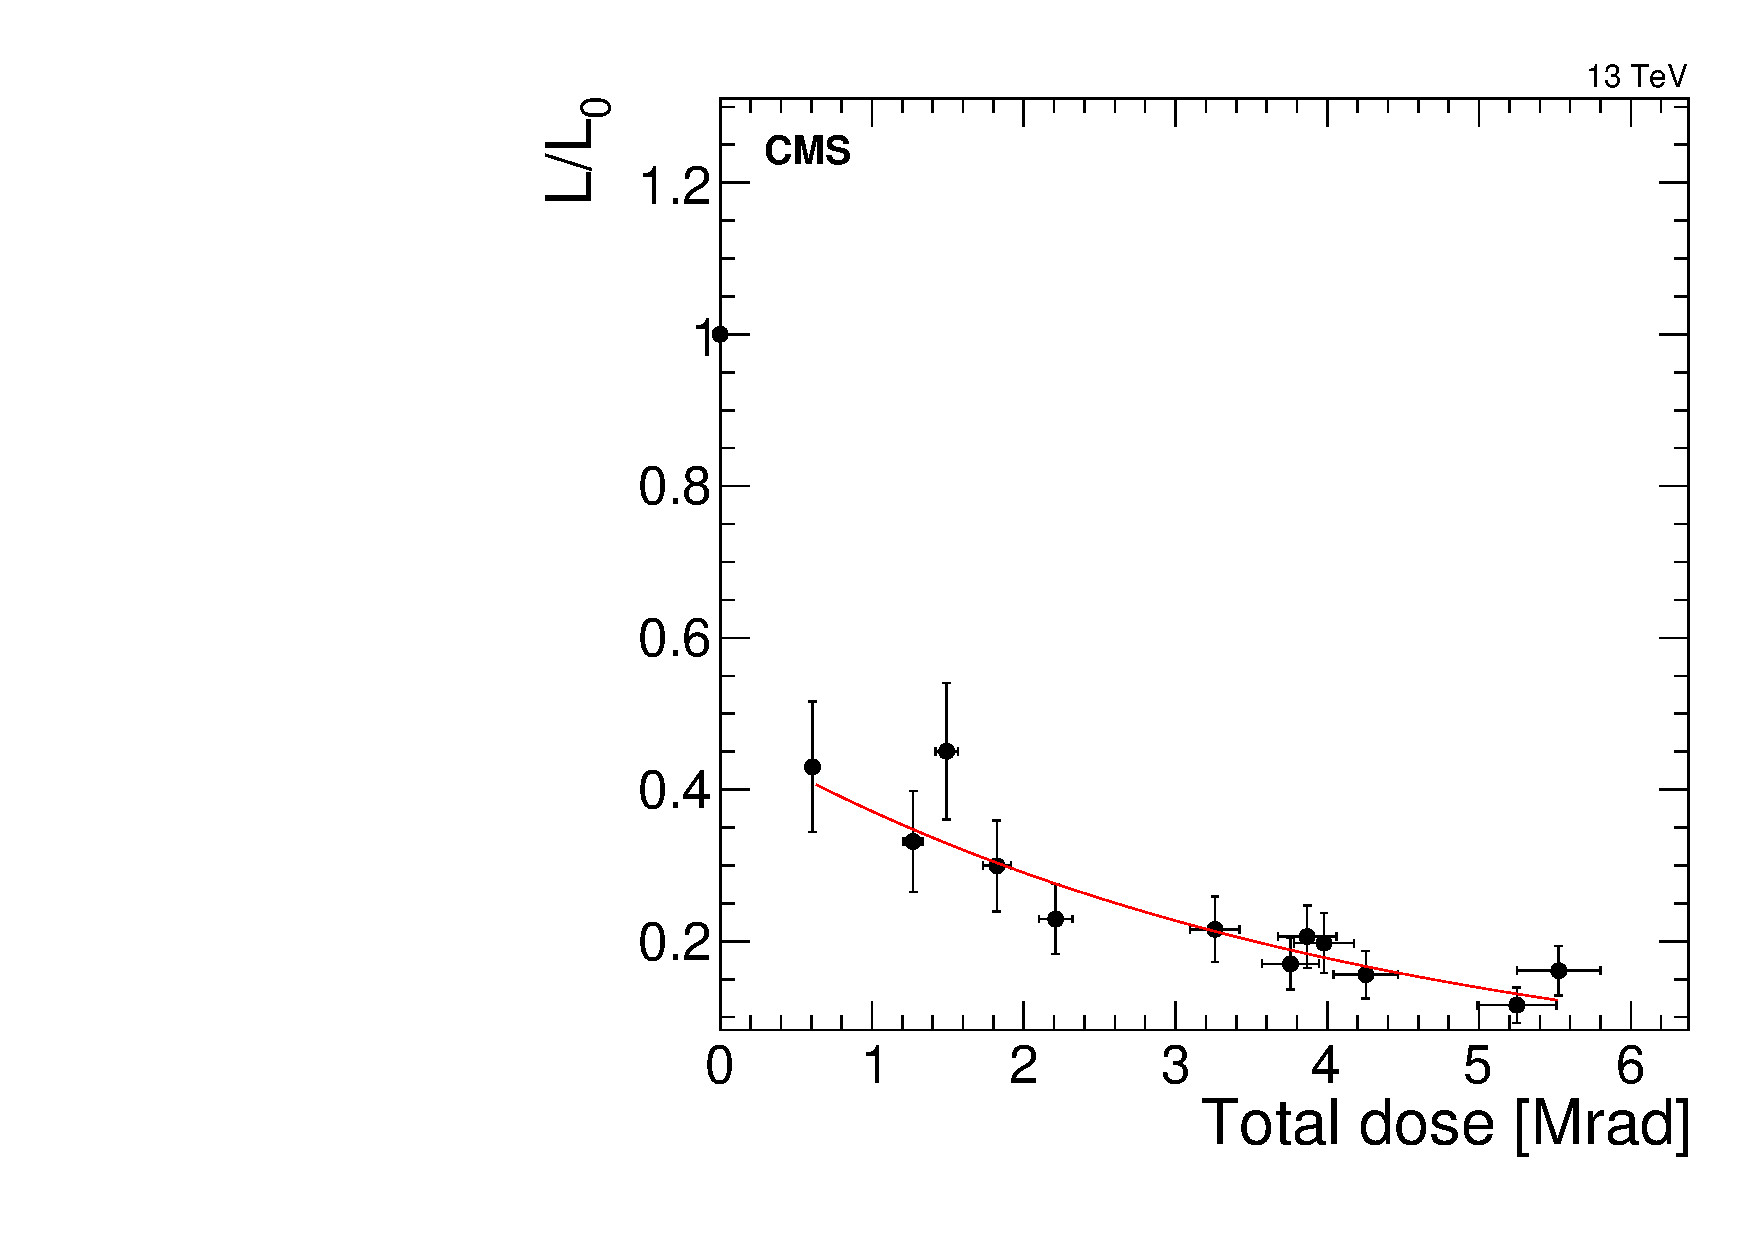
\includegraphics[width=0.45\textwidth]{figures/SCSN81-S-13p1cm-f7ch5-dose.pdf}
\caption{Relative yield versus integrated dose for SCSN81 sigma tiles at 11.8 cm (top left and right) and 13.1 cm (bottom) from the CMS beam pipe, receiving 16.61 krad/hr and 15.23 krad/hr respectively. The exponential decay curve fitted to the steady-state region of light loss is shown in red.}
\label{fig:SCSN81-S-11p8cm-dose}
\end{figure} 

\begin{figure}[tbp!]
\centering
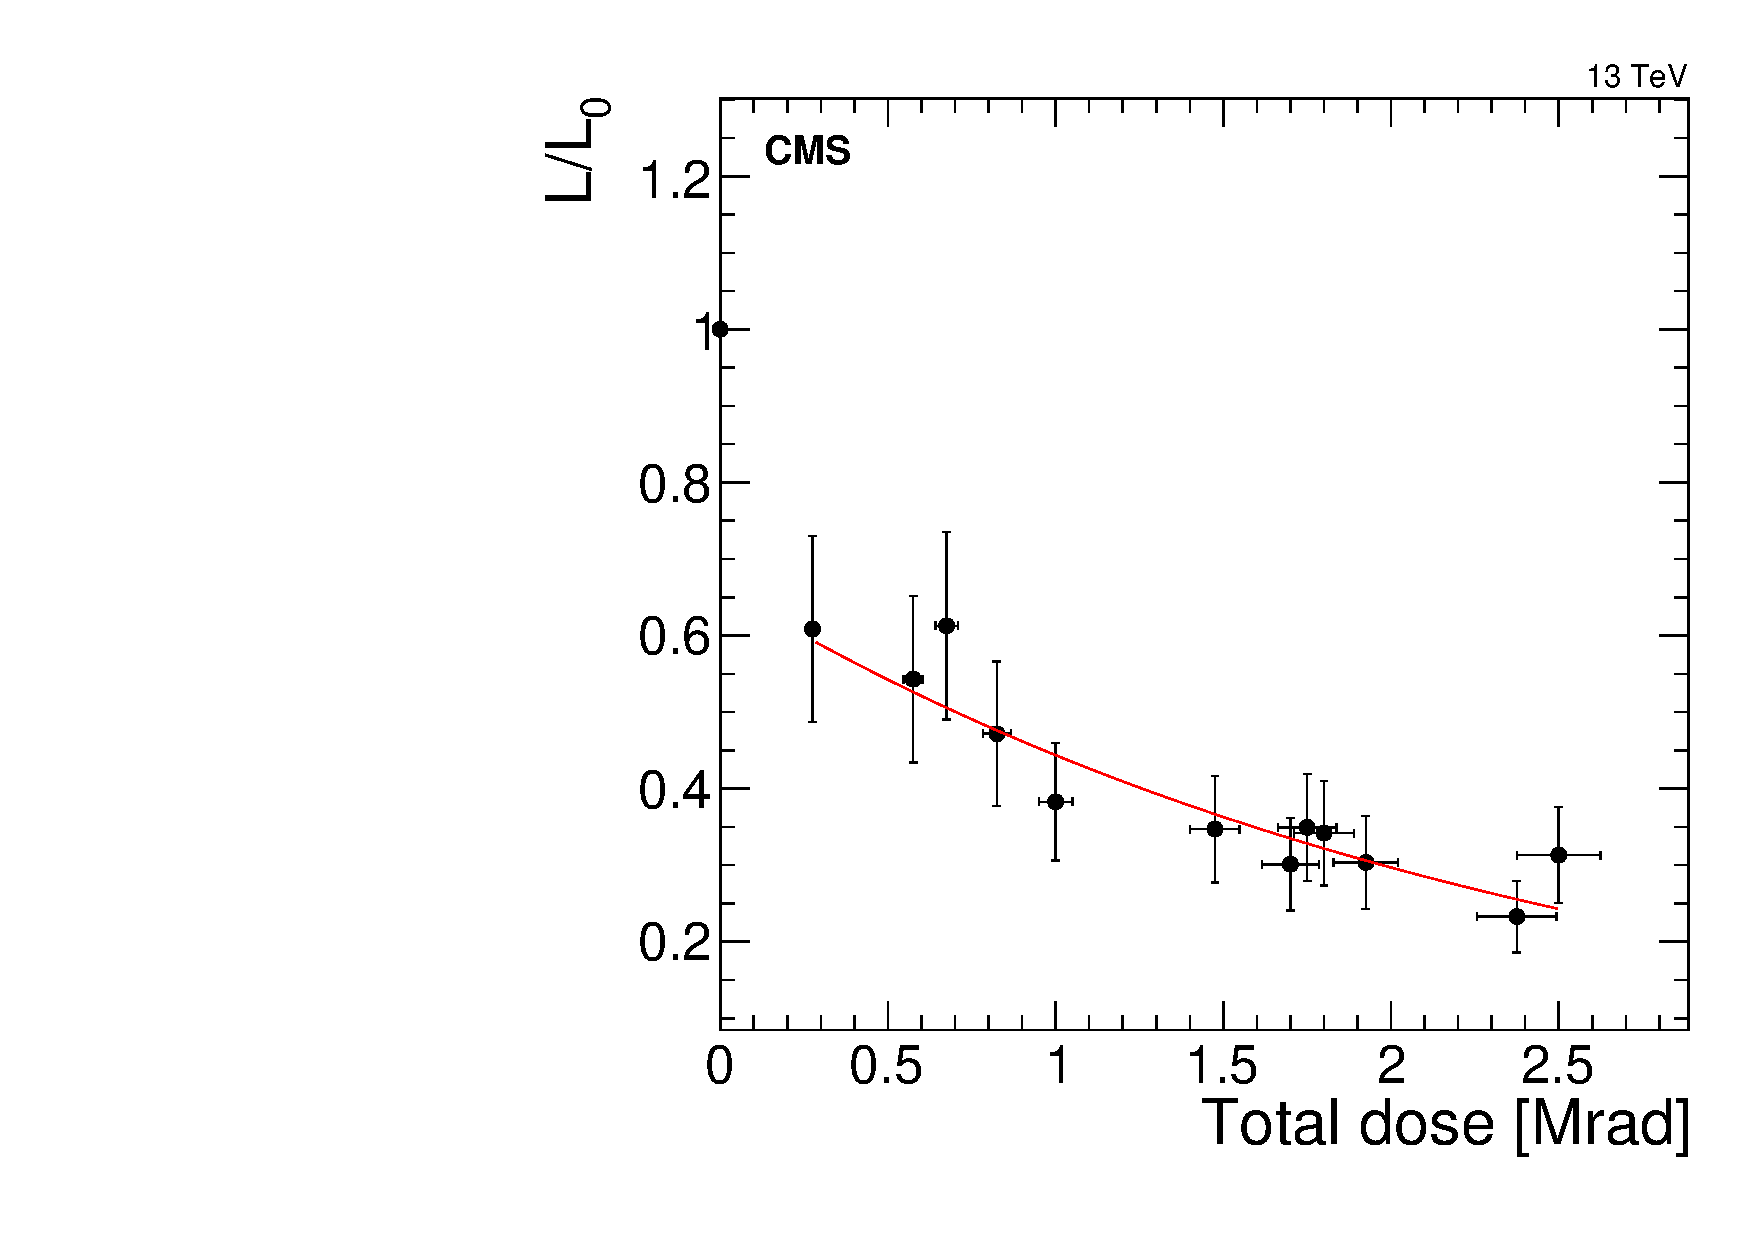
\includegraphics[width=0.45\textwidth]{figures/SCSN81-S-18p2cm-f5ch0-dose.pdf}
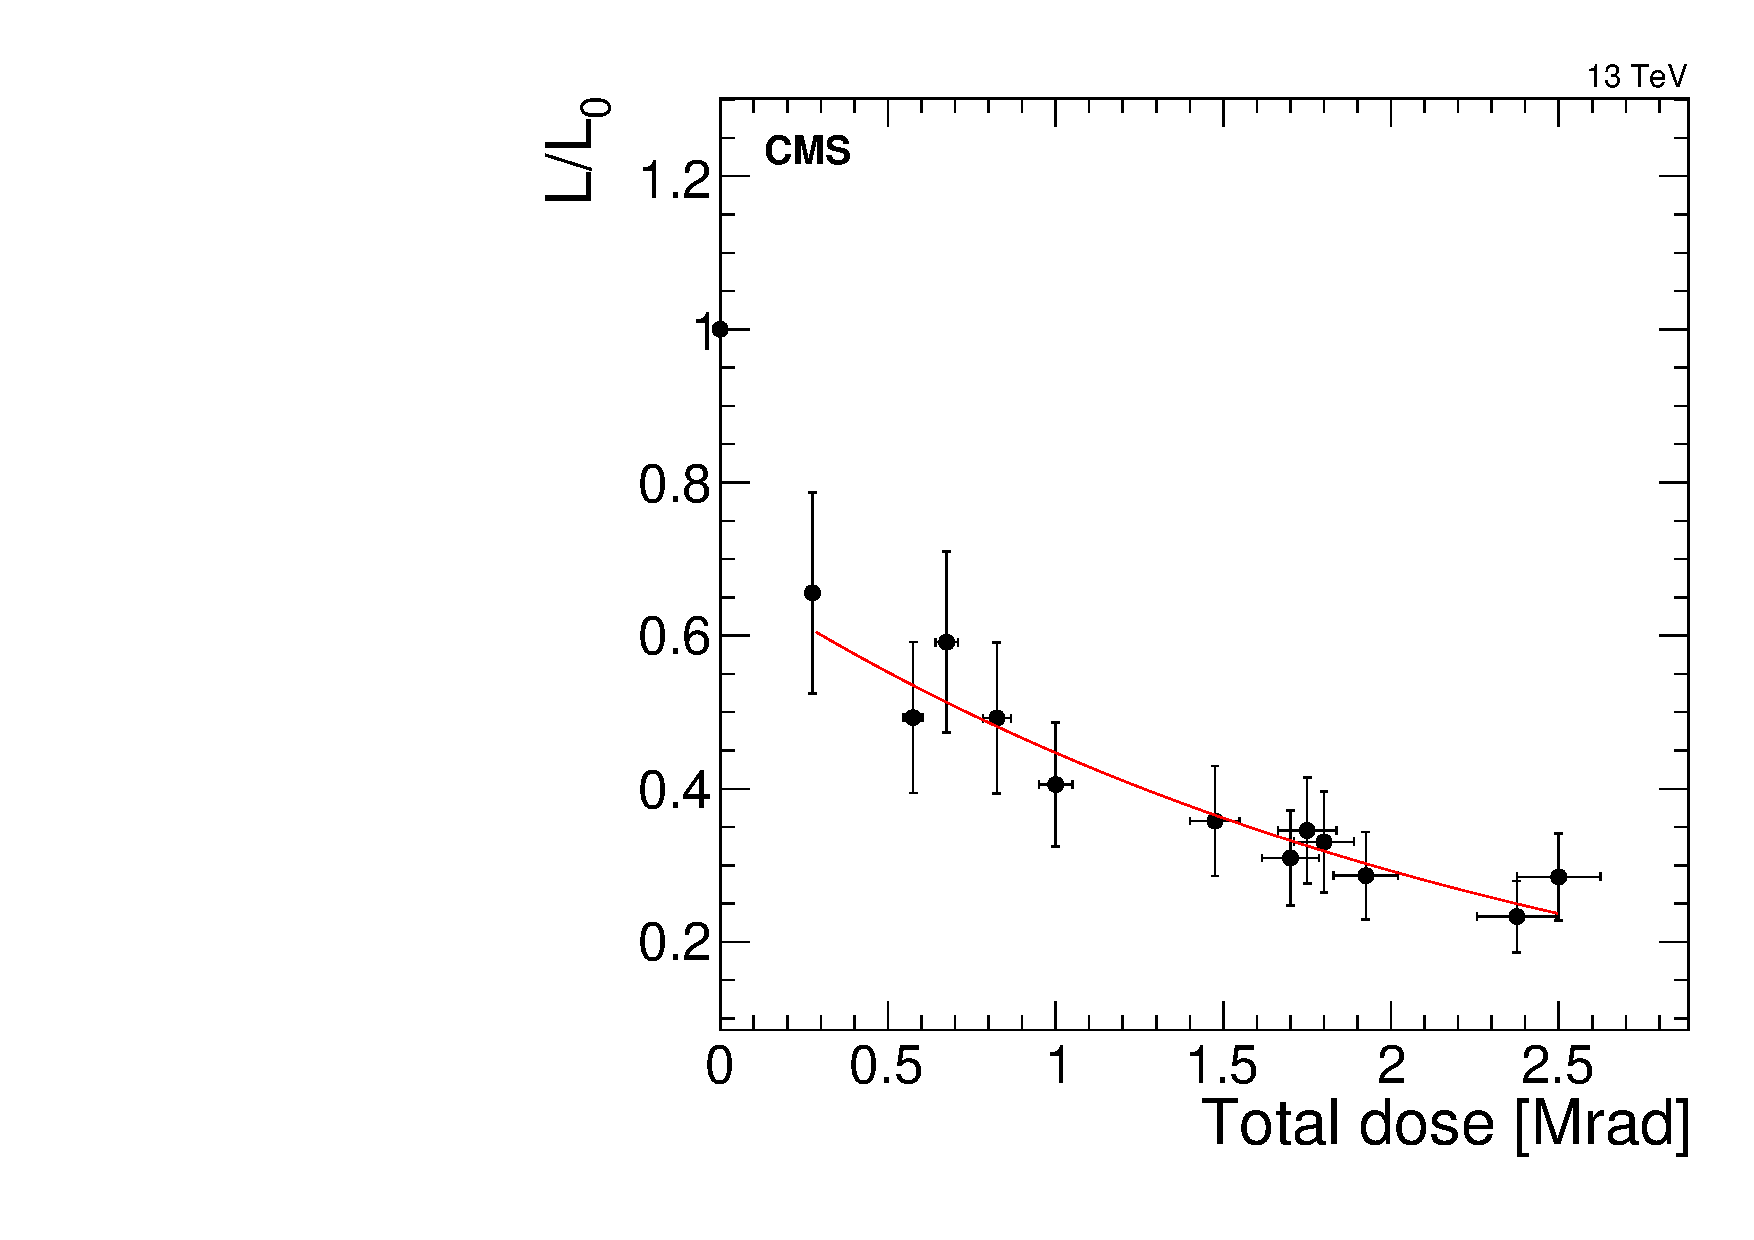
\includegraphics[width=0.45\textwidth]{figures/SCSN81-S-18p2cm-f20ch5-dose.pdf}
\caption{Relative yield versus integrated dose for SCSN81 sigma tiles at 18.2 cm from the CMS beam pipe, receiving 6.89 krad/hr. The exponential decay curve fitted to the steady-state region of light loss is shown in red.}
\label{fig:SCSN81-S-18p2cm-dose}
\end{figure} 

\begin{figure}[tbp!]
\centering
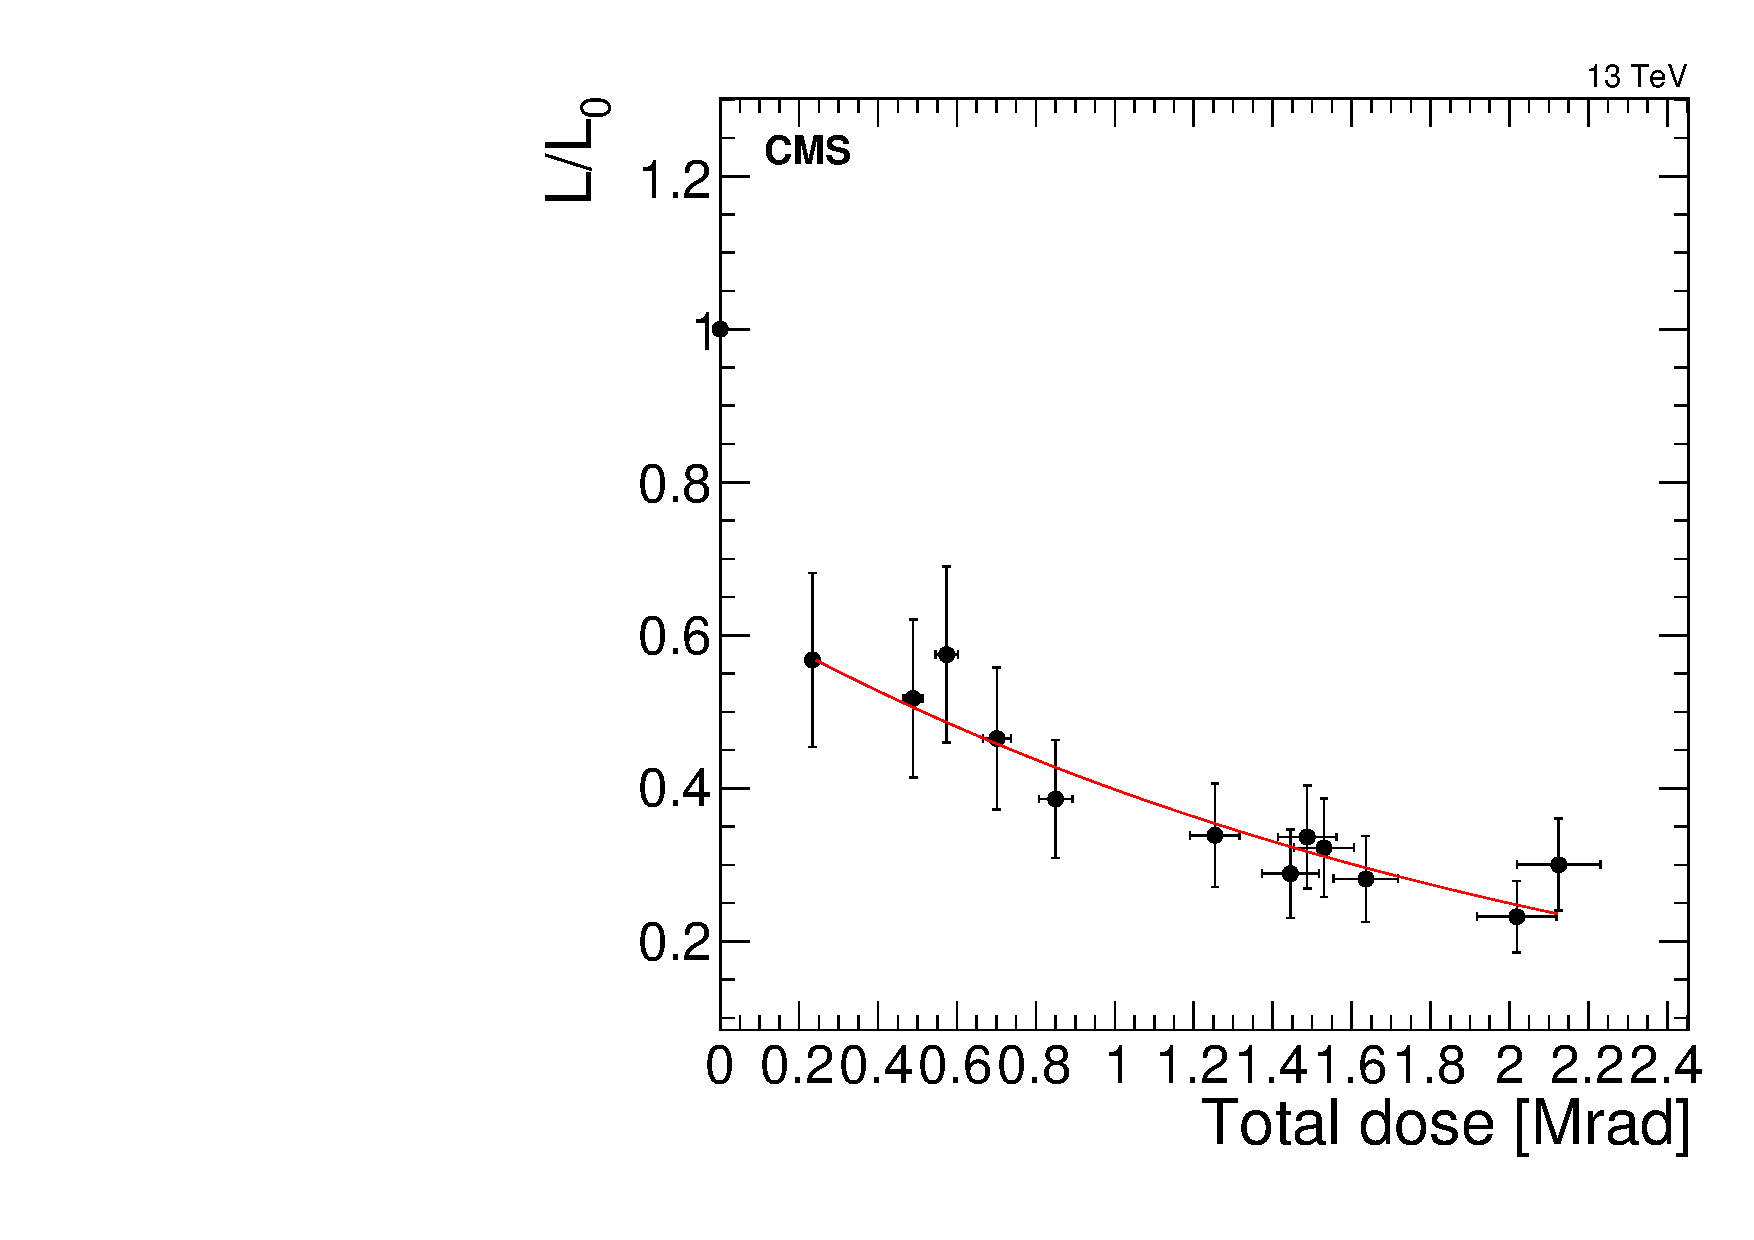
\includegraphics[width=0.45\textwidth]{figures/SCSN81-S-19p5cm-f2ch1-dose.pdf}
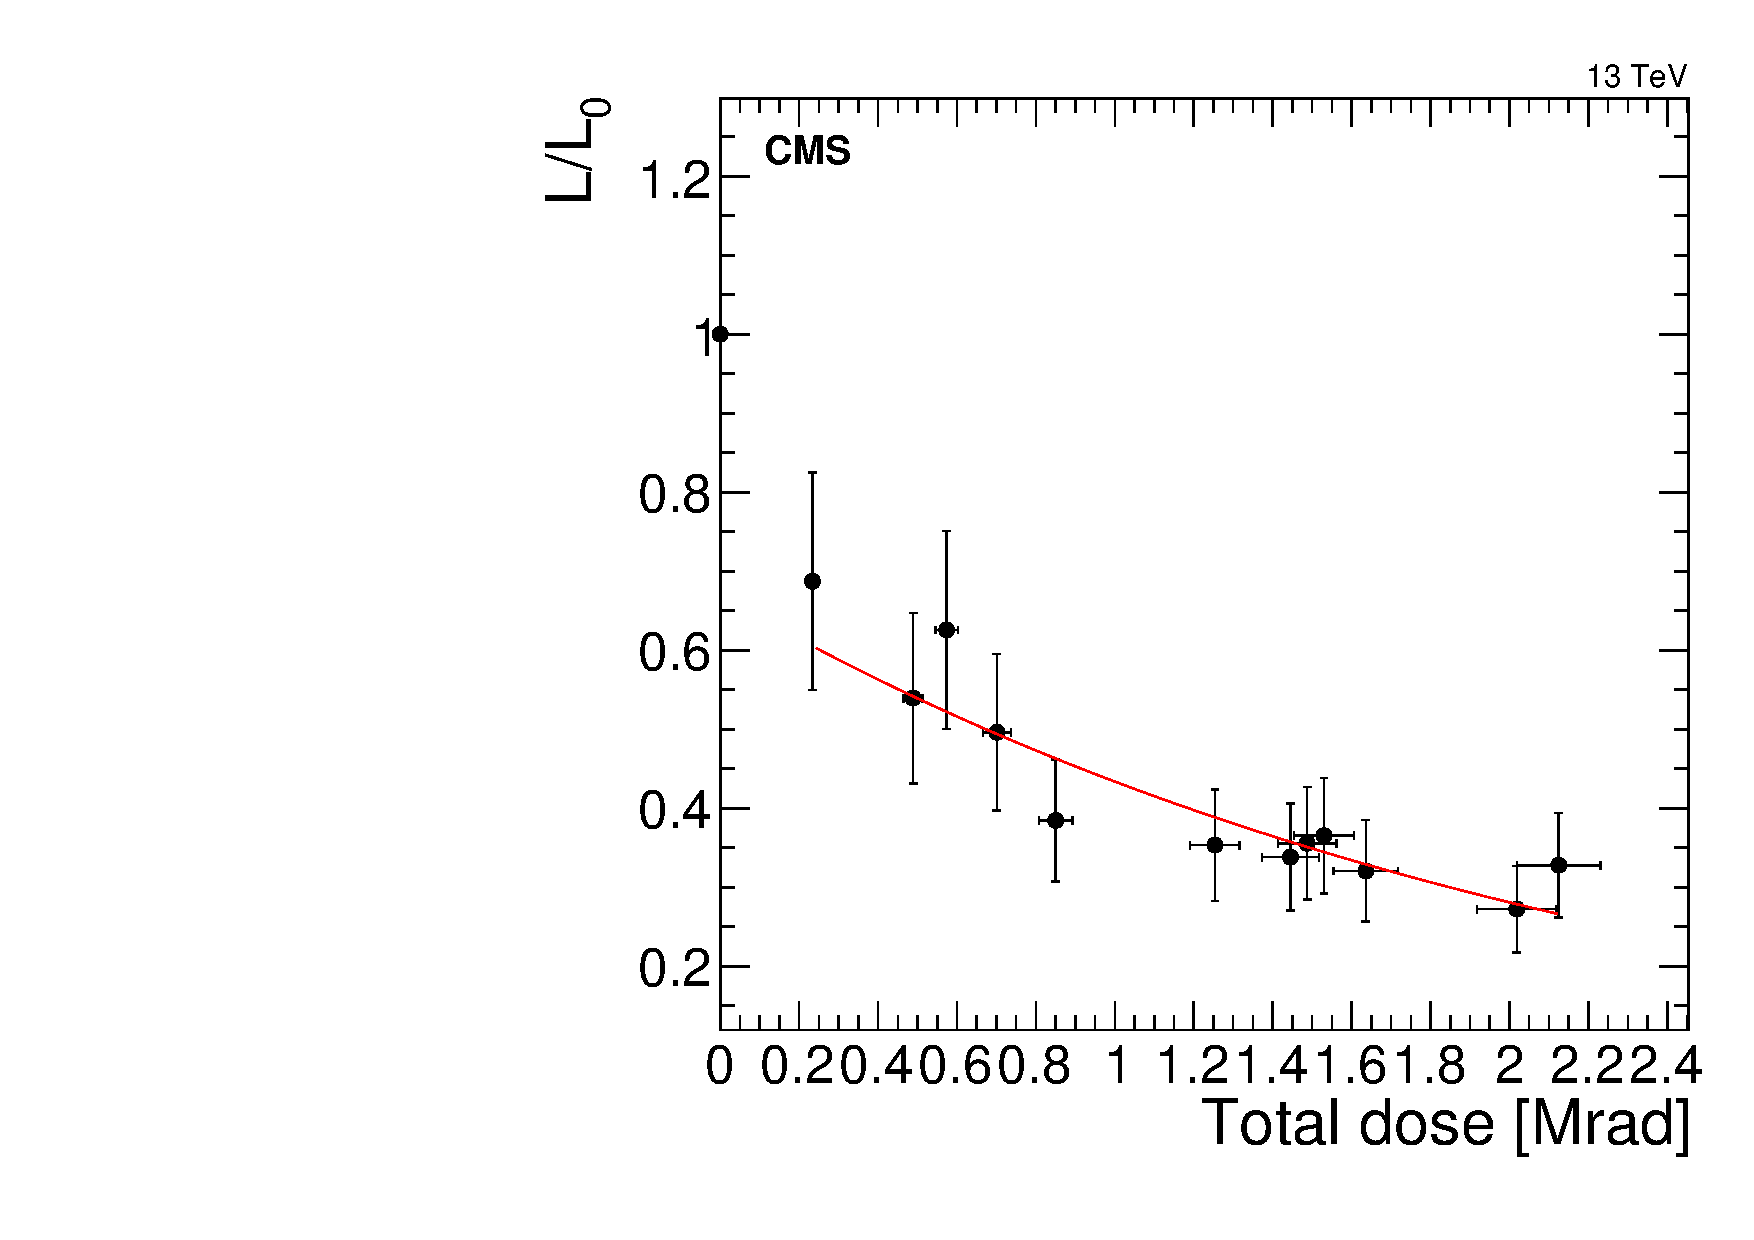
\includegraphics[width=0.45\textwidth]{figures/SCSN81-S-19p5cm-f15ch1-dose.pdf}
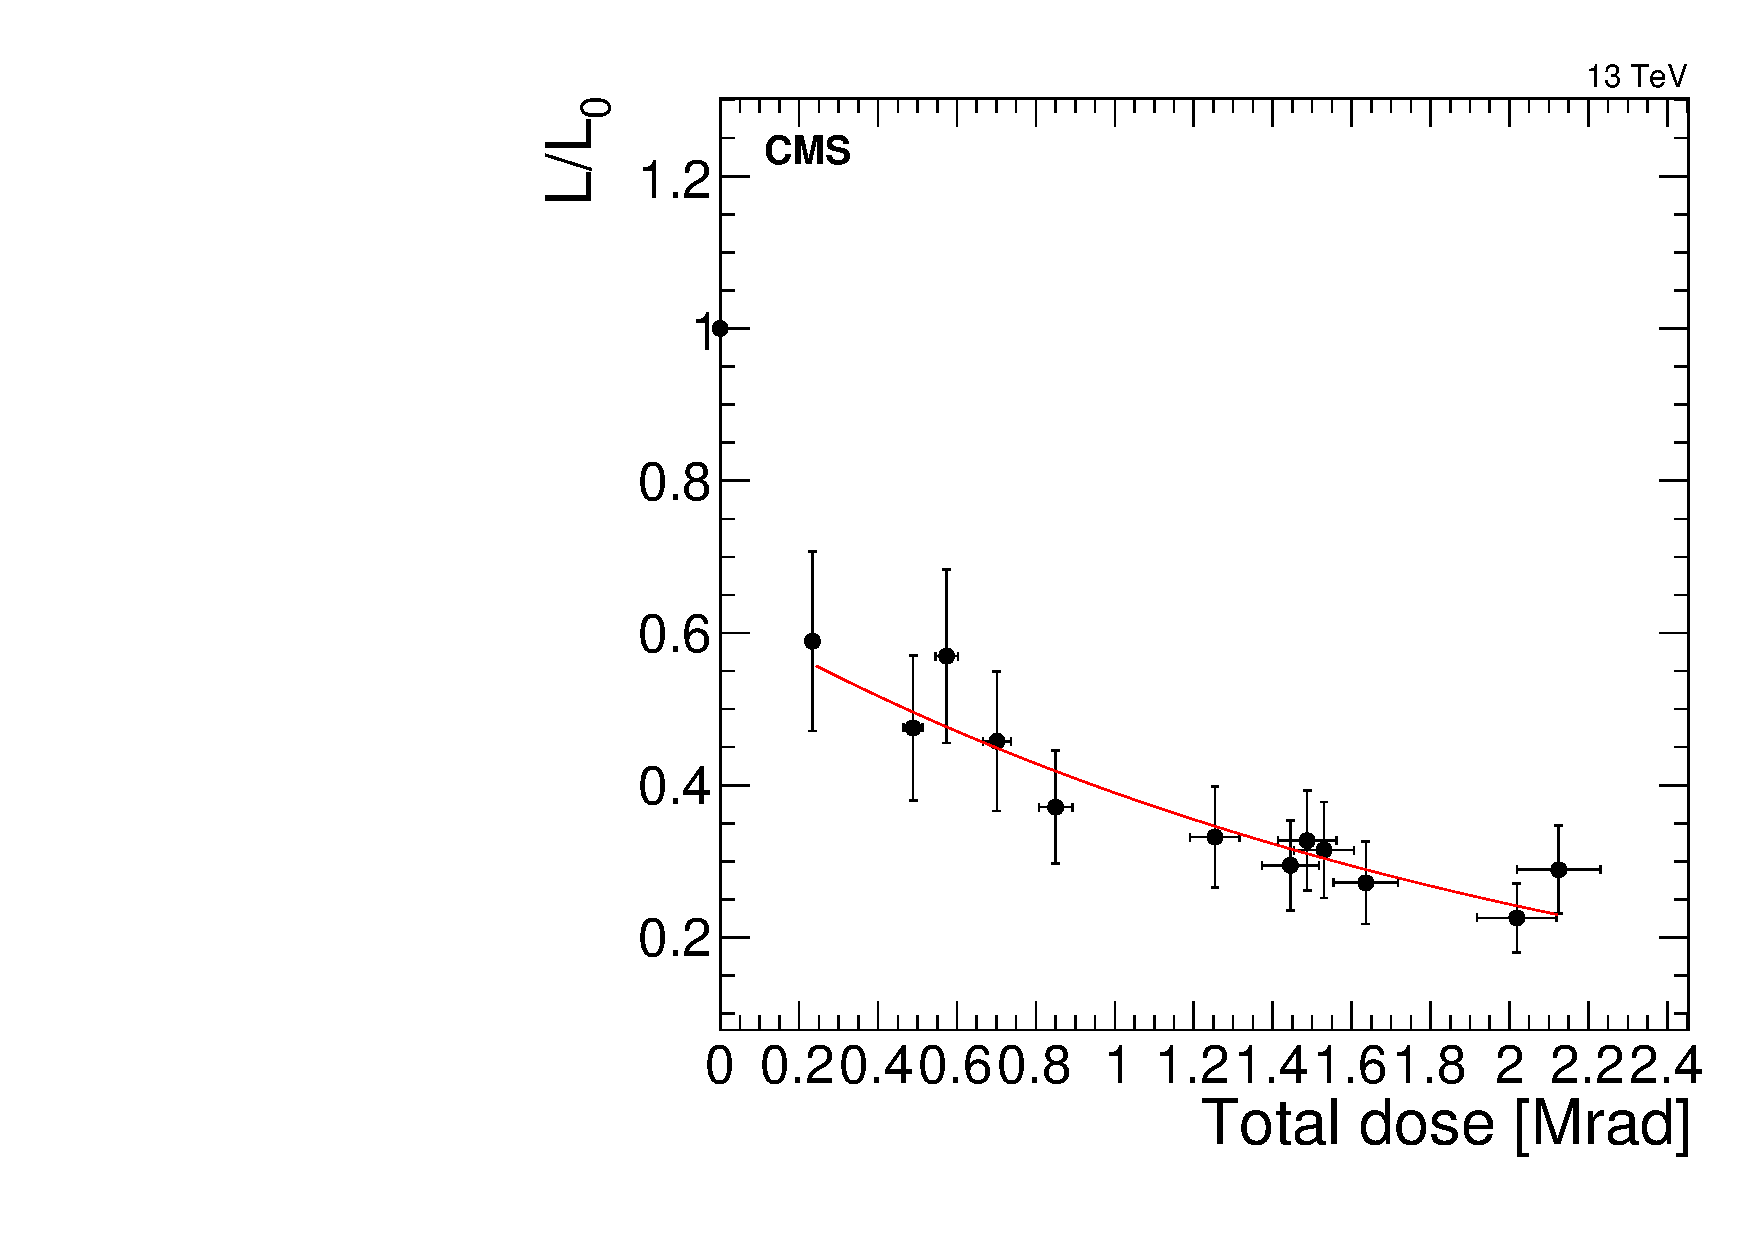
\includegraphics[width=0.45\textwidth]{figures/SCSN81-S-19p5cm-f20ch4-dose.pdf}
\caption{Relative yield versus integrated dose for SCSN81 sigma tiles at 19.5 cm from the CMS beam pipe, receiving 5.86 krad/hr. The exponential decay curve fitted to the steady-state region of light loss is shown in red.}
\label{fig:SCSN81-S-19p5cm-dose}
\end{figure} 

\begin{figure}[tbp!]
\centering
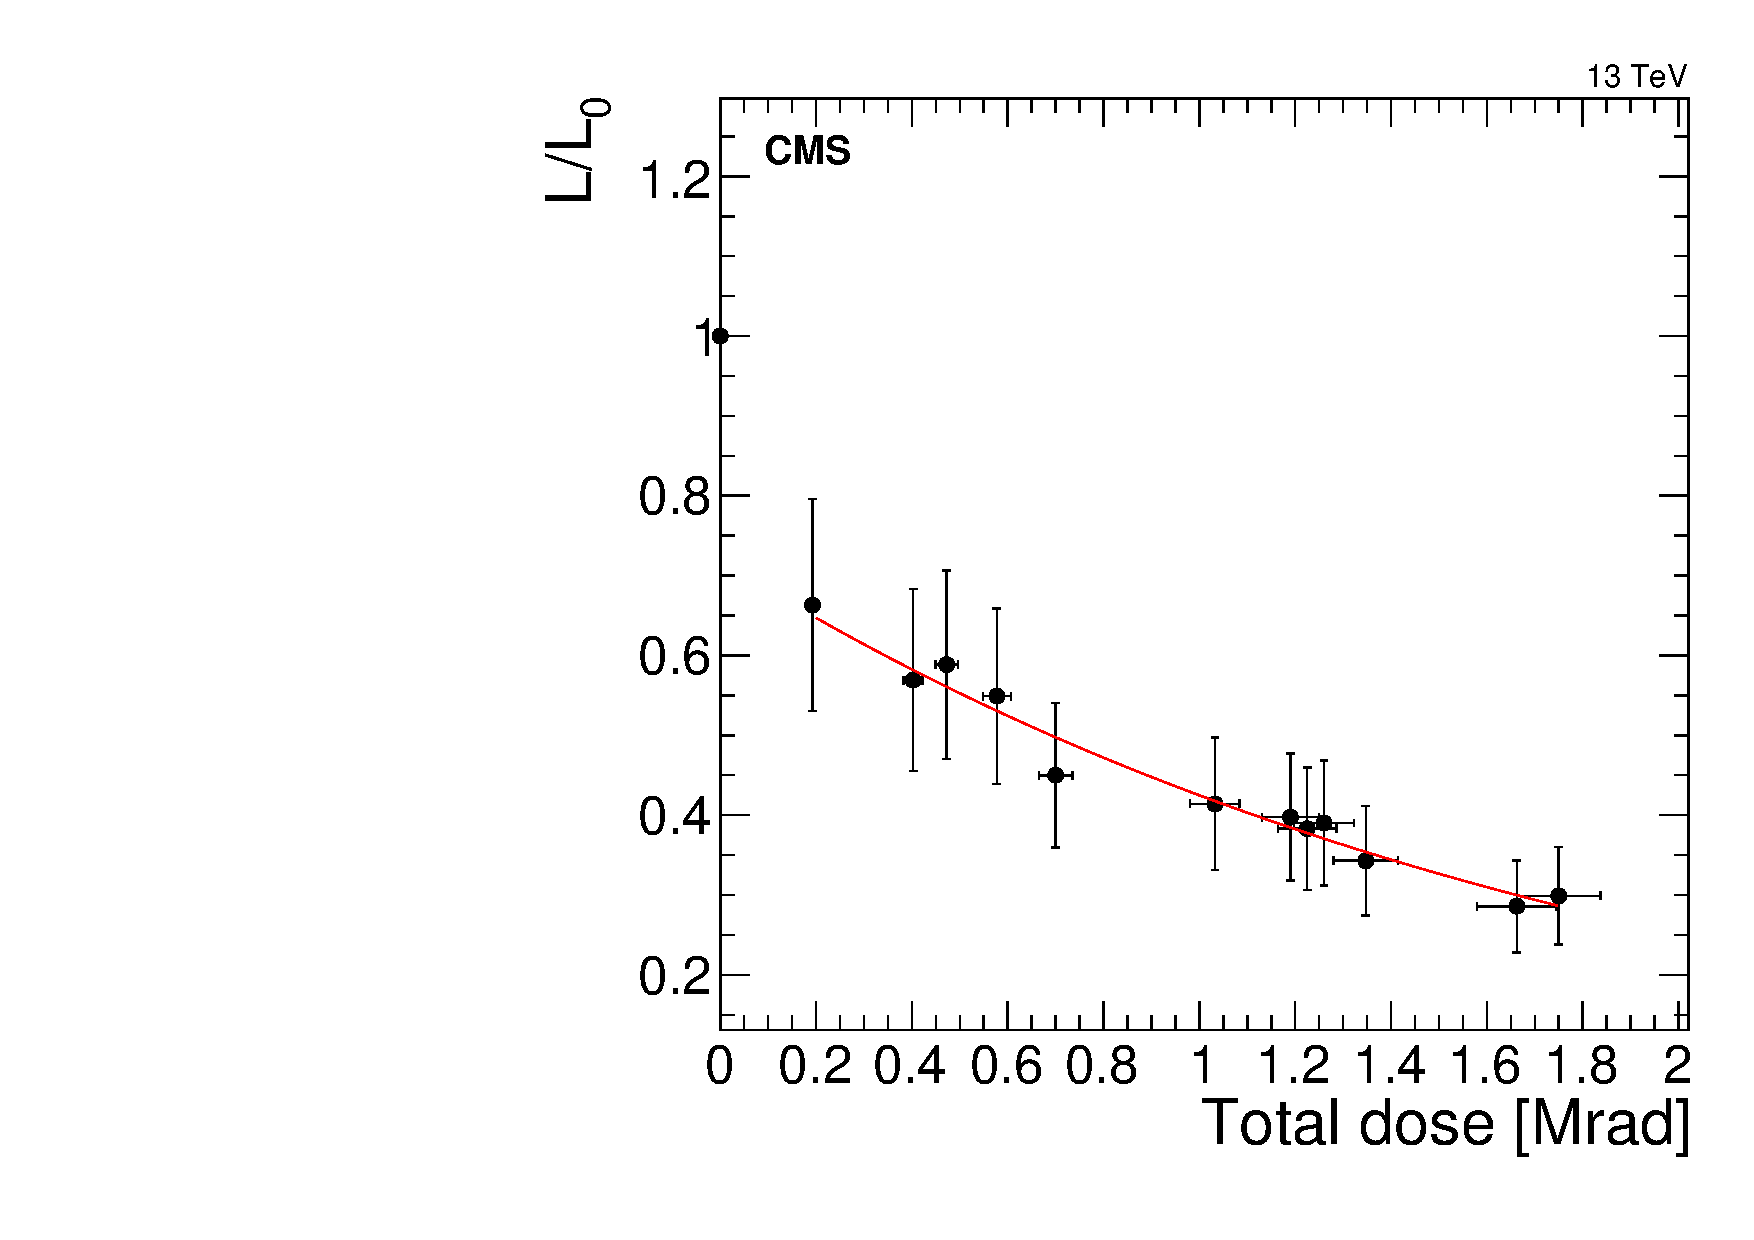
\includegraphics[width=0.45\textwidth]{figures/SCSN81-S-24p6cm-f3ch2-dose.pdf}
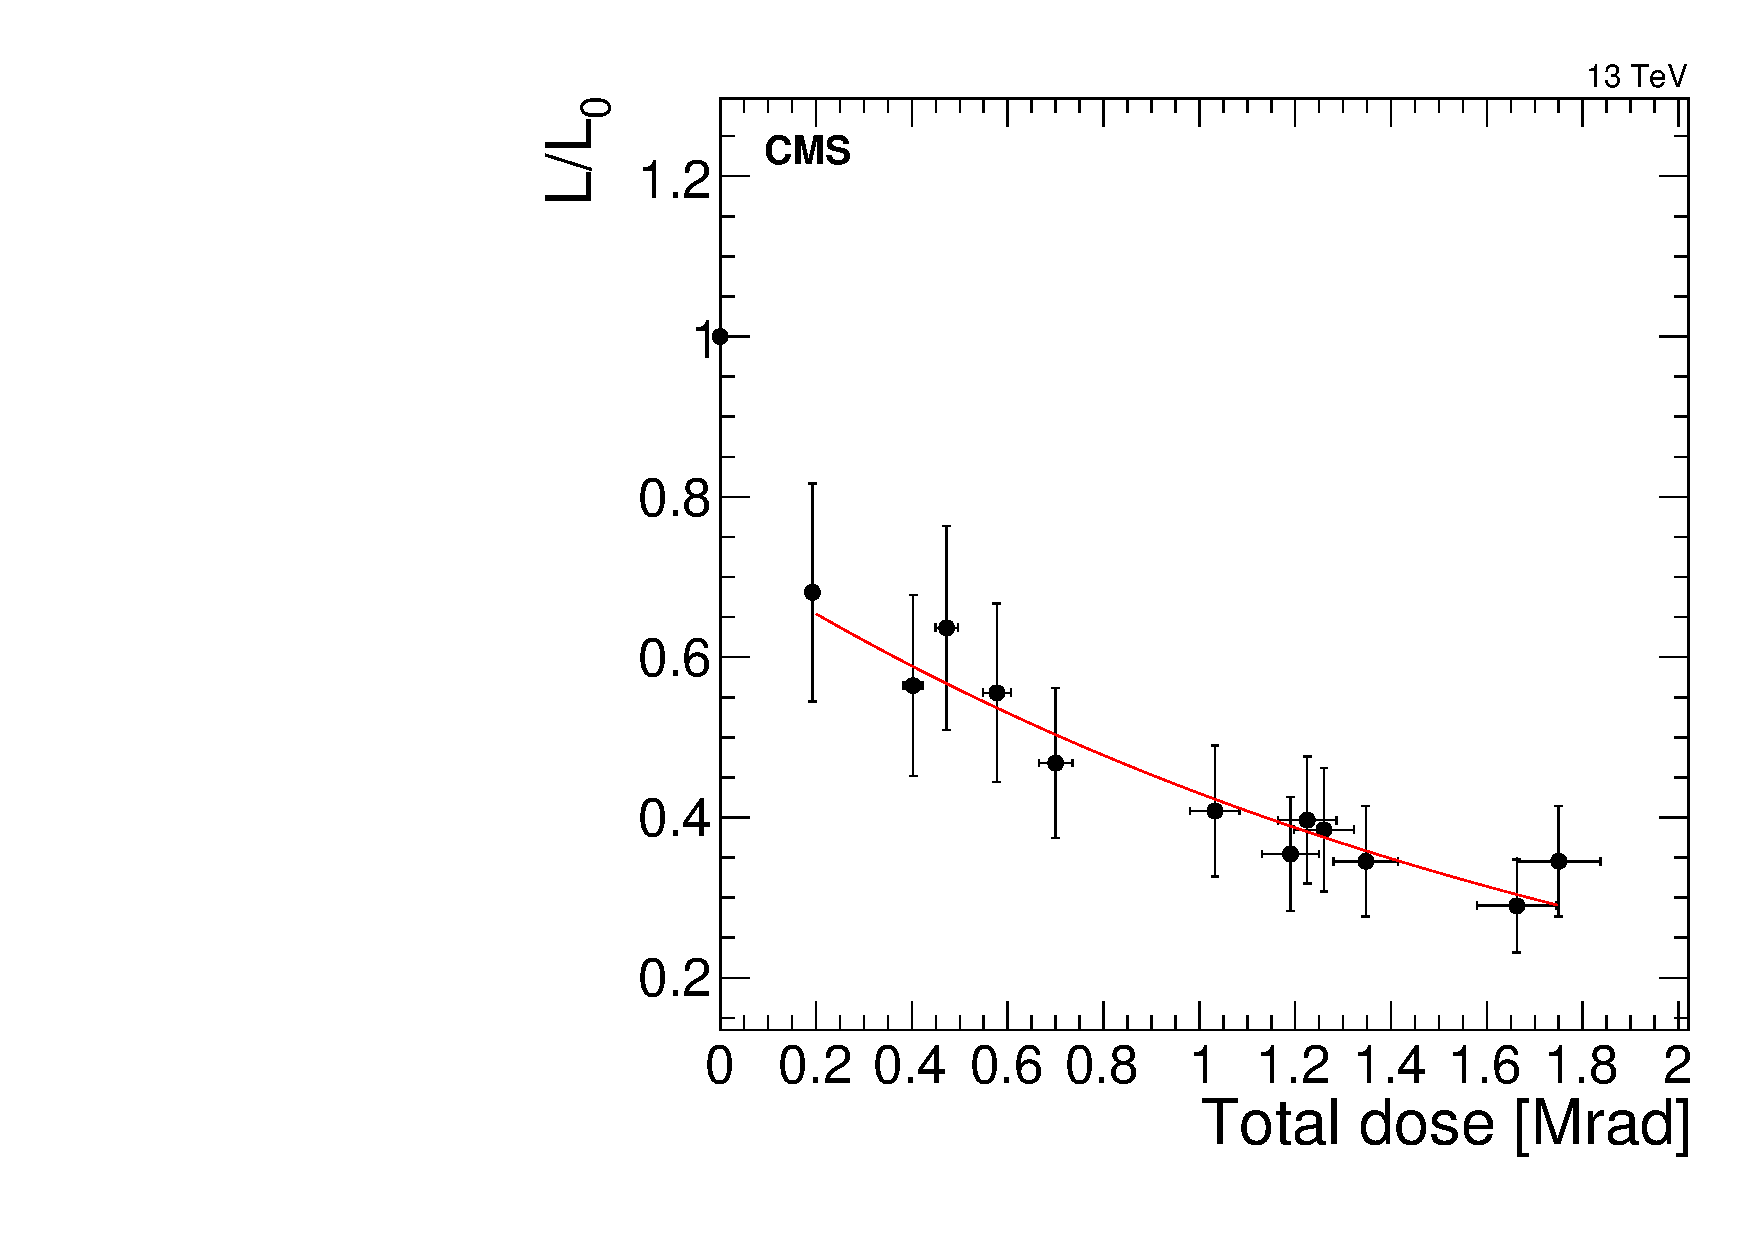
\includegraphics[width=0.45\textwidth]{figures/SCSN81-S-24p6cm-f14ch4-dose.pdf}
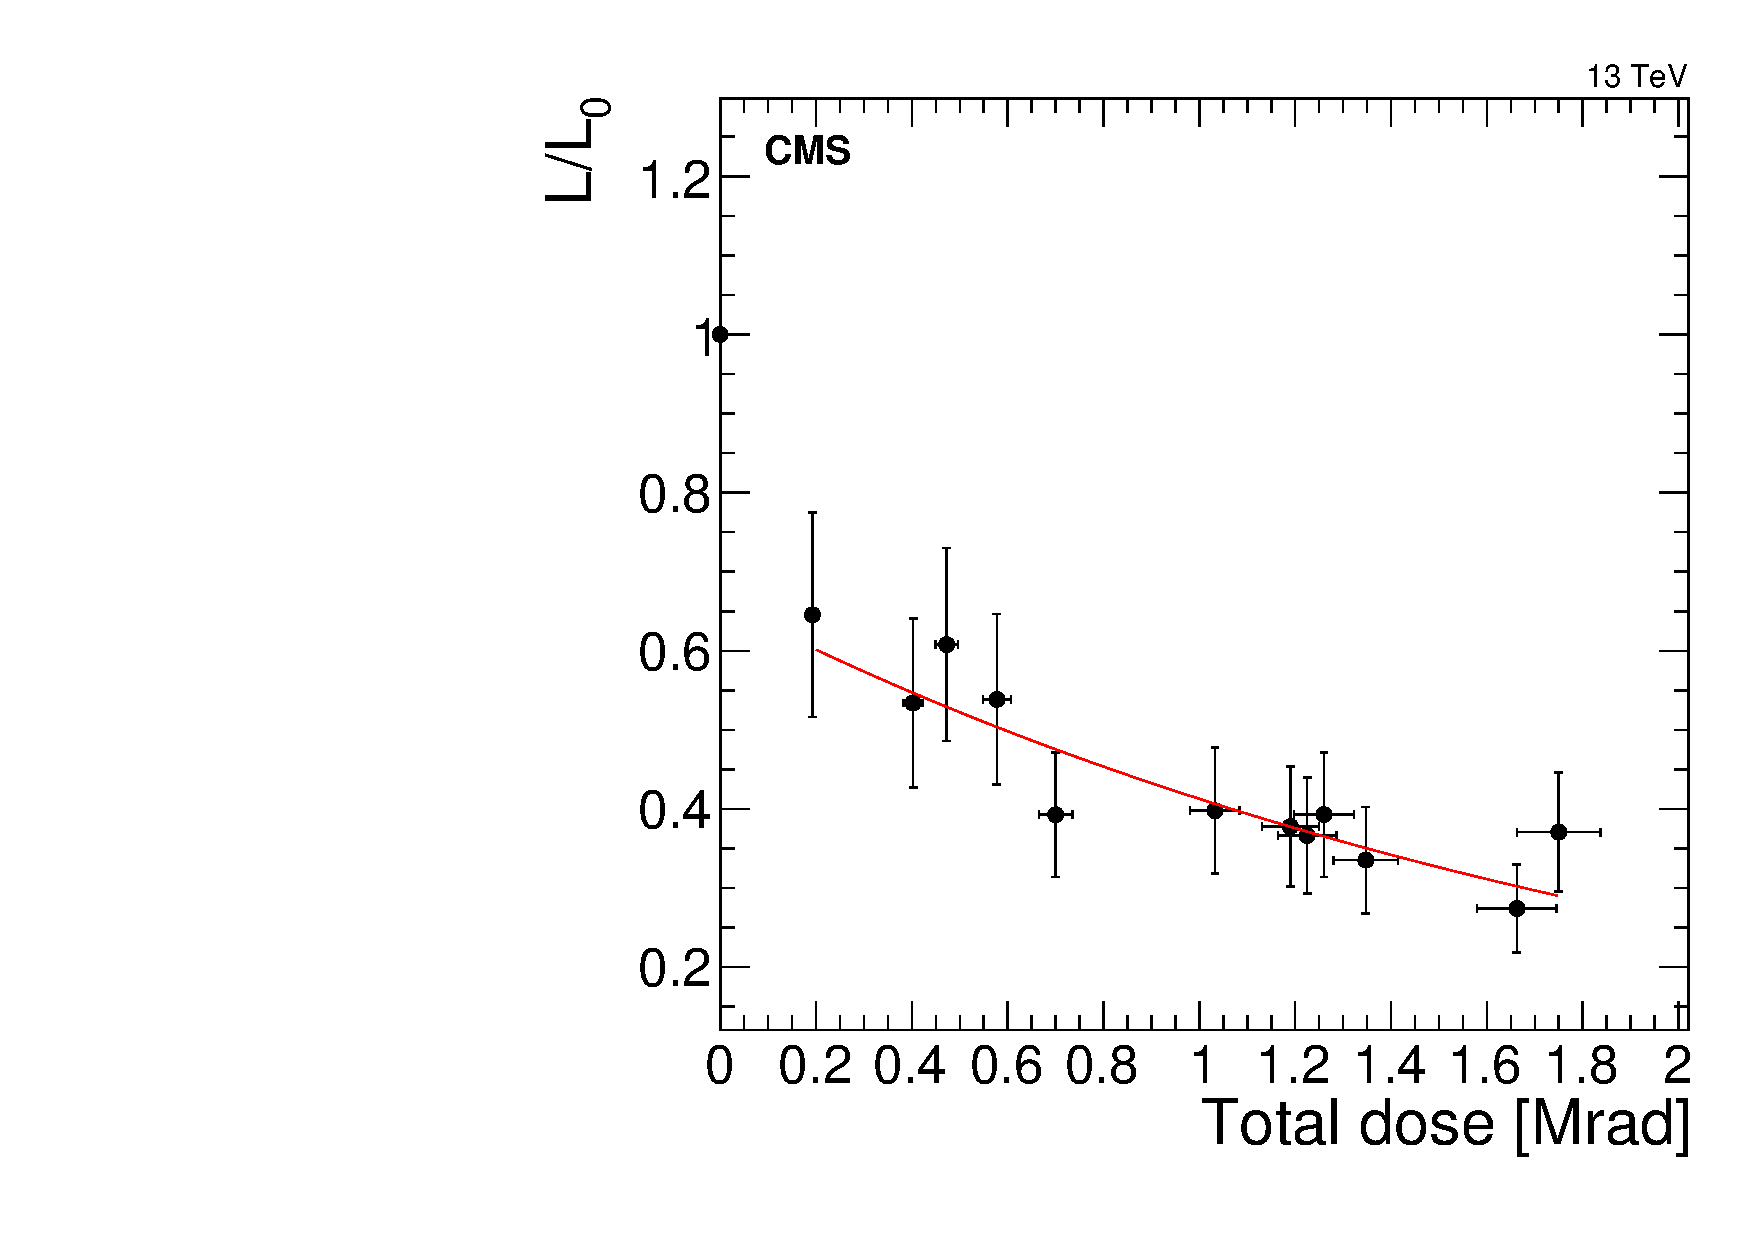
\includegraphics[width=0.45\textwidth]{figures/SCSN81-S-24p6cm-f15ch4-dose.pdf}
\caption{Relative yield versus integrated dose for SCSN81 sigma tiles at 24.6 cm from the CMS beam pipe, receiving 4.82 krad/hr. The exponential decay curve fitted to the steady-state region of light loss is shown in red.}
\label{fig:SCSN81-S-24p6cm-dose}
\end{figure} 

\begin{figure}[tbp!]
\centering
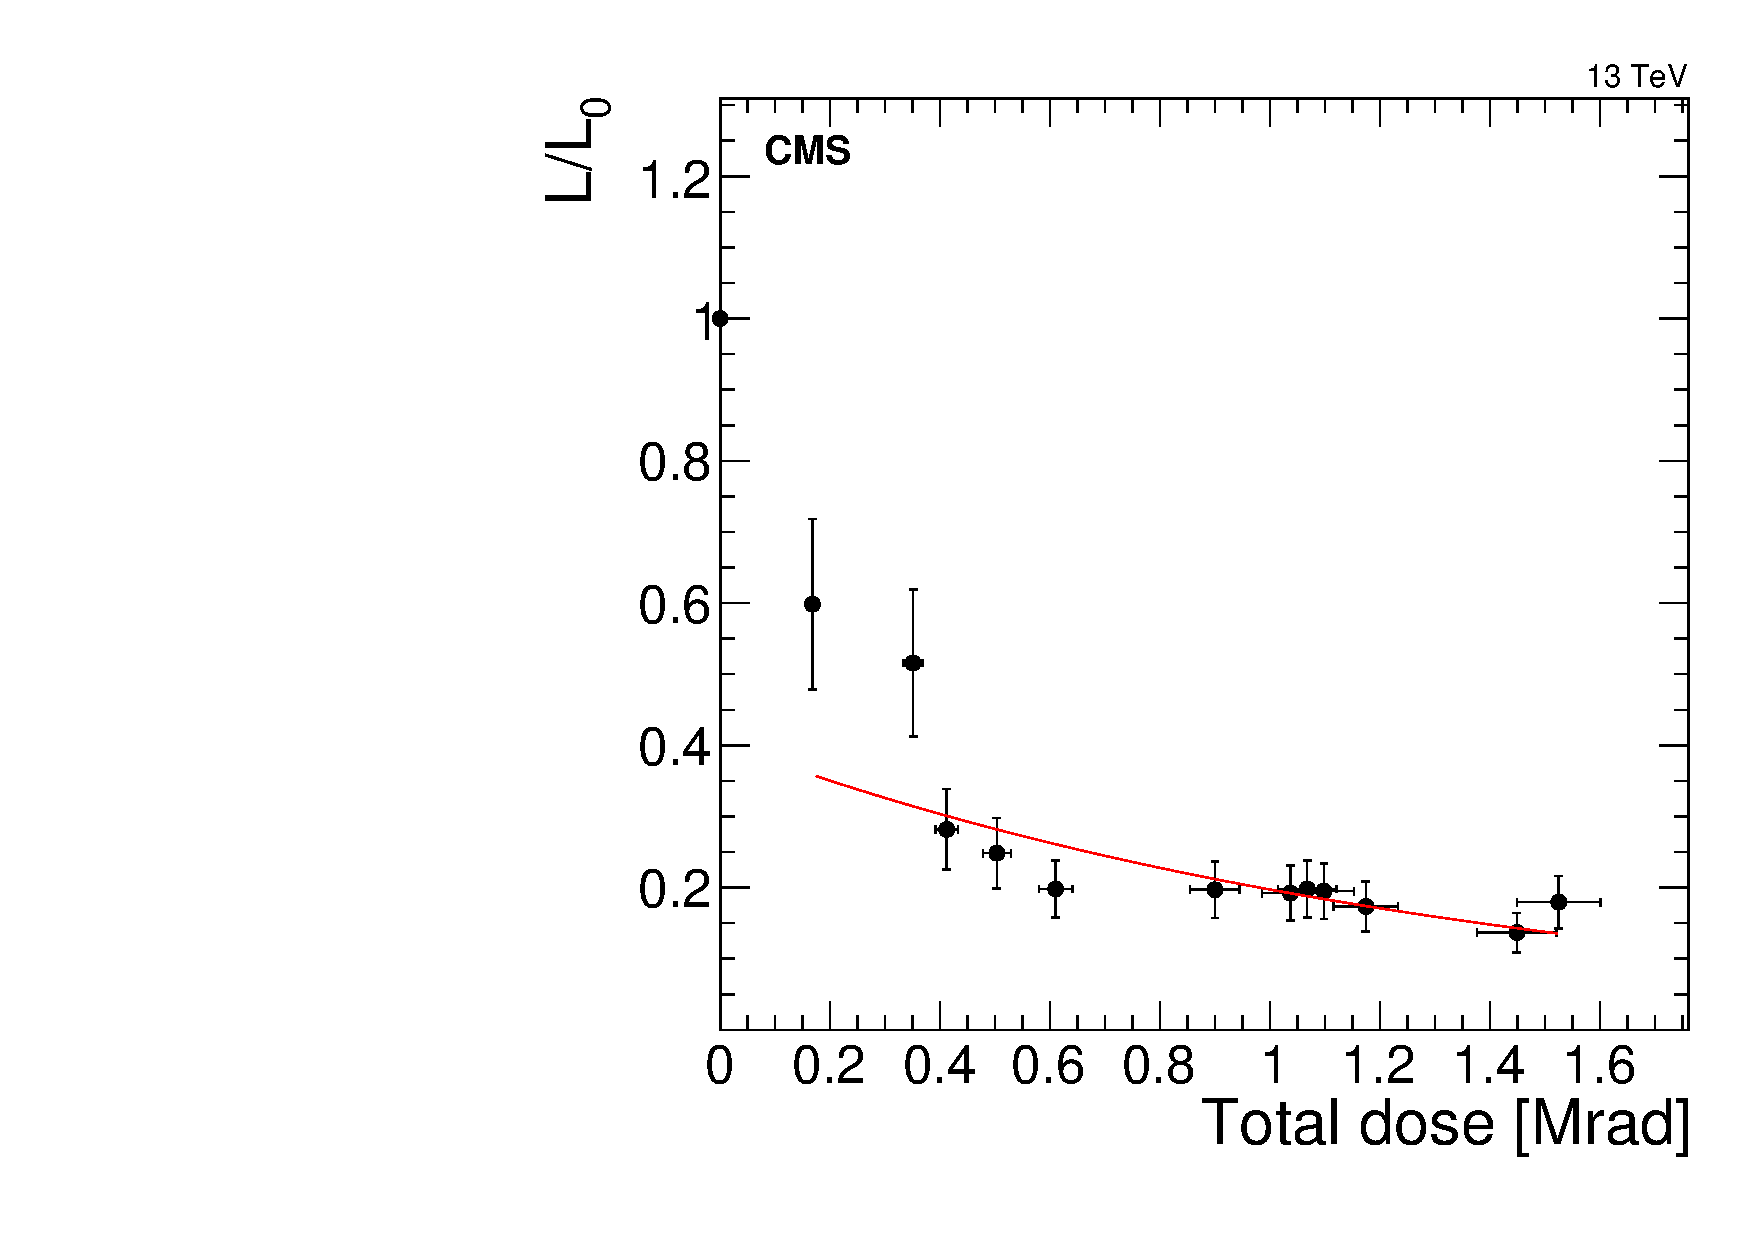
\includegraphics[width=0.45\textwidth]{figures/SCSN81-S-25p9cm-f7ch2-dose.pdf}
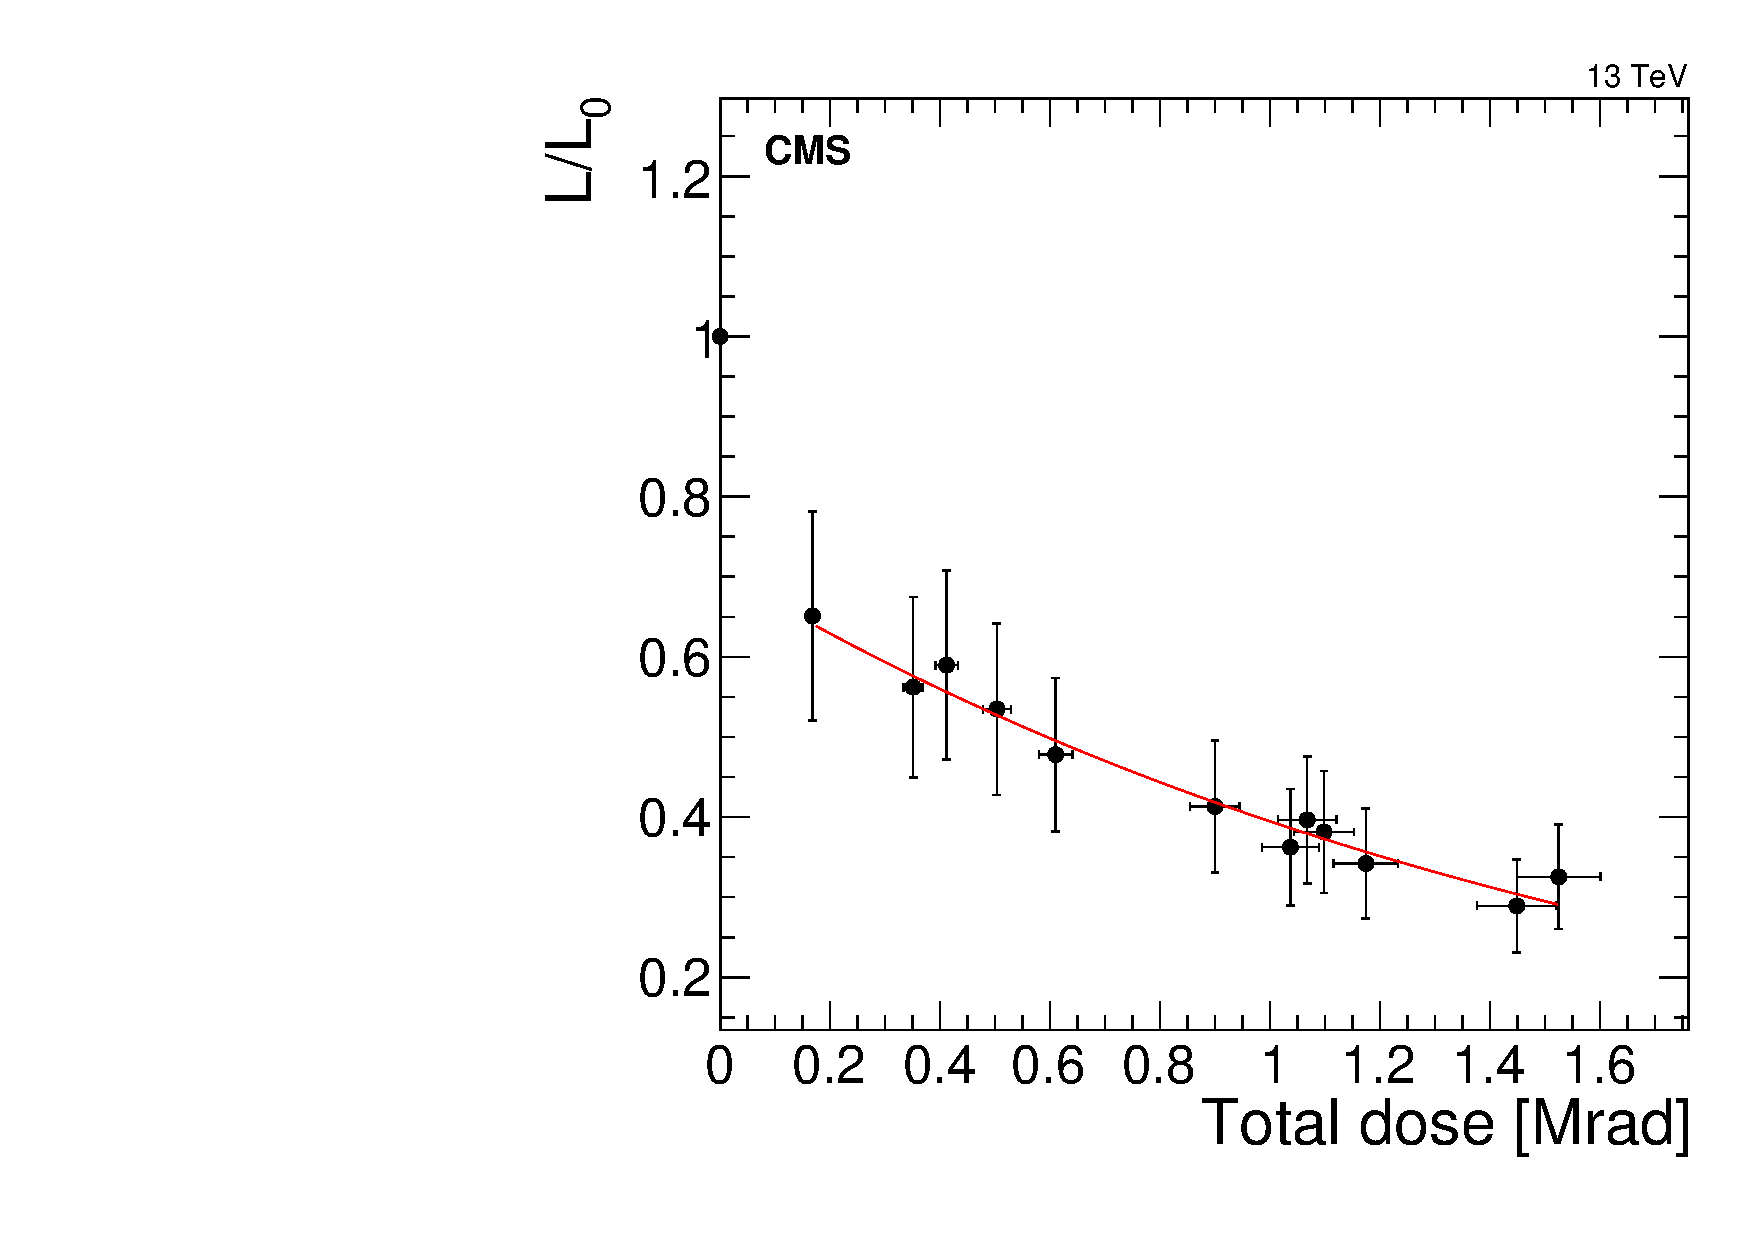
\includegraphics[width=0.45\textwidth]{figures/SCSN81-S-25p9cm-f8ch5-dose.pdf}
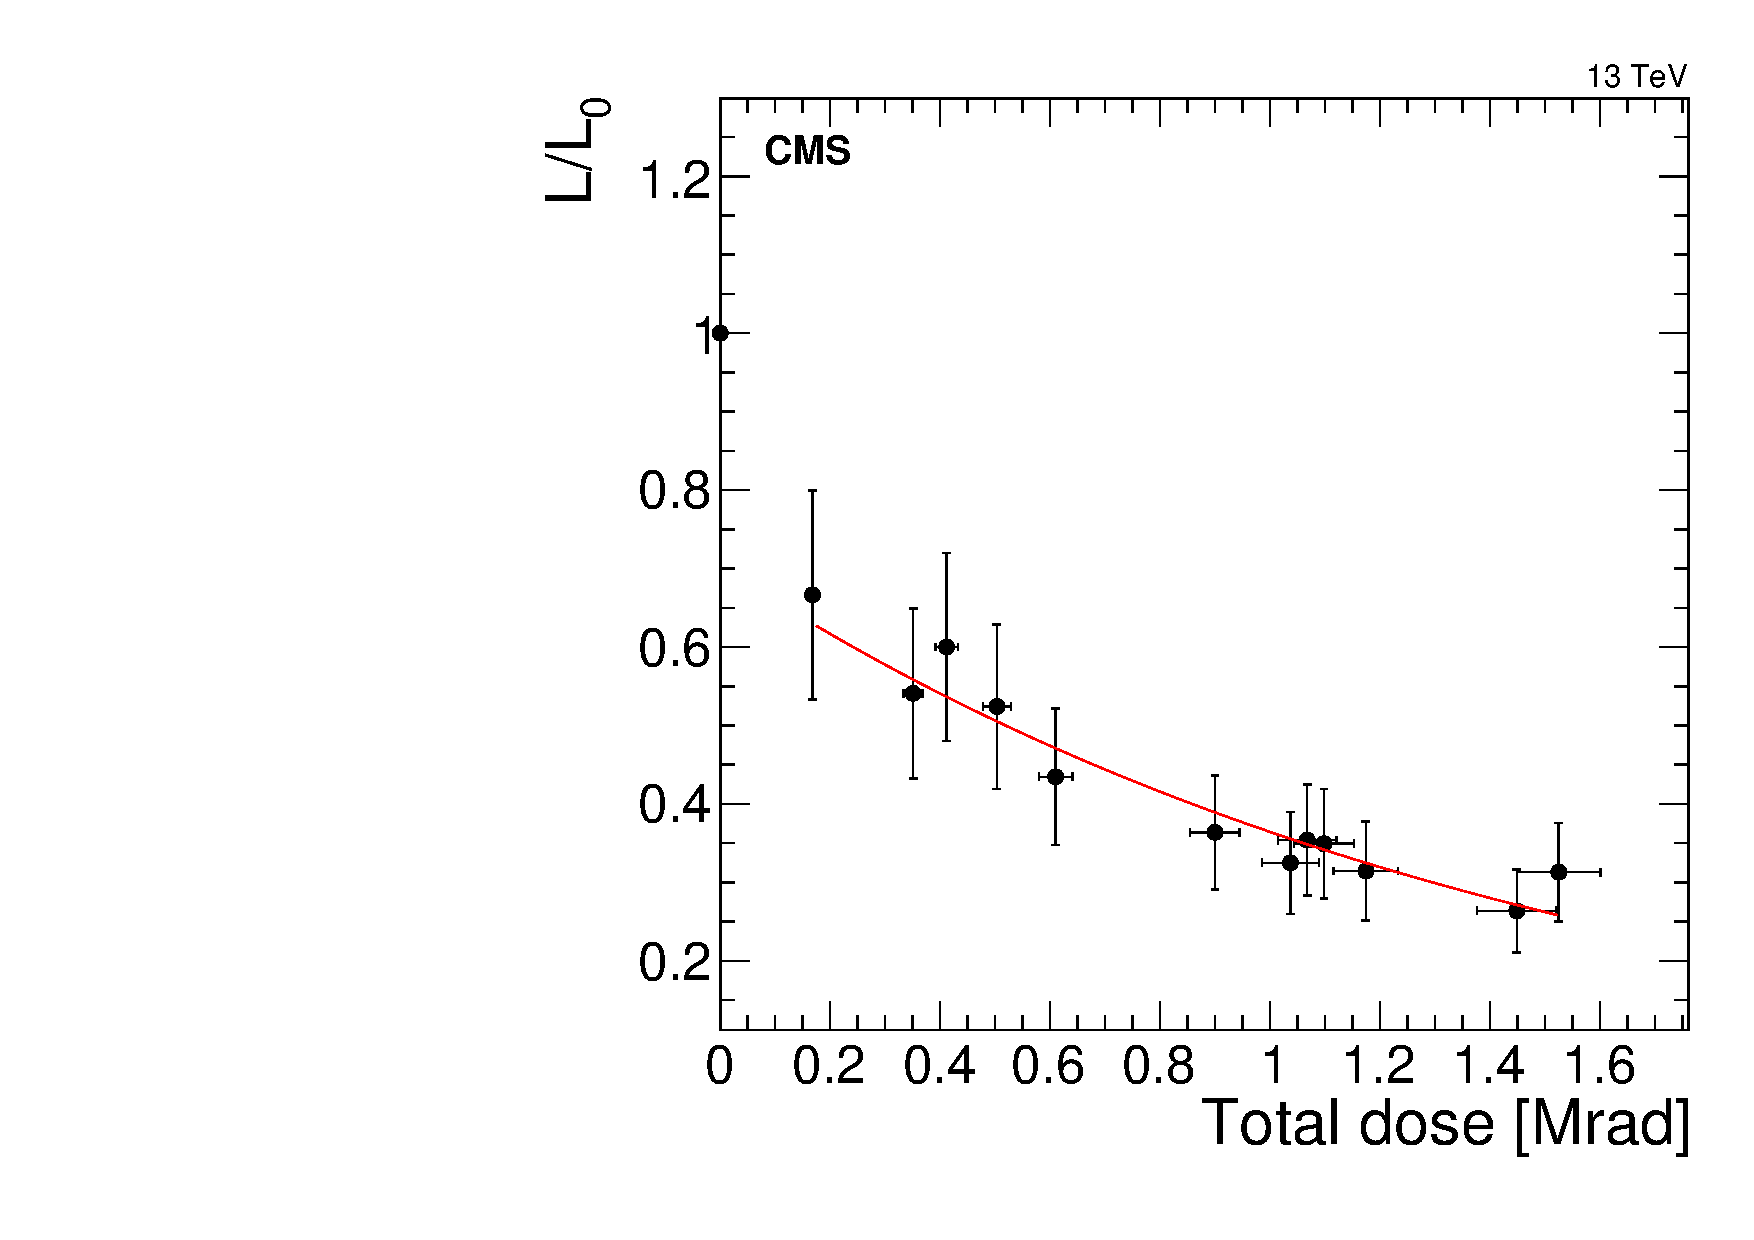
\includegraphics[width=0.45\textwidth]{figures/SCSN81-S-25p9cm-f14ch3-dose.pdf}
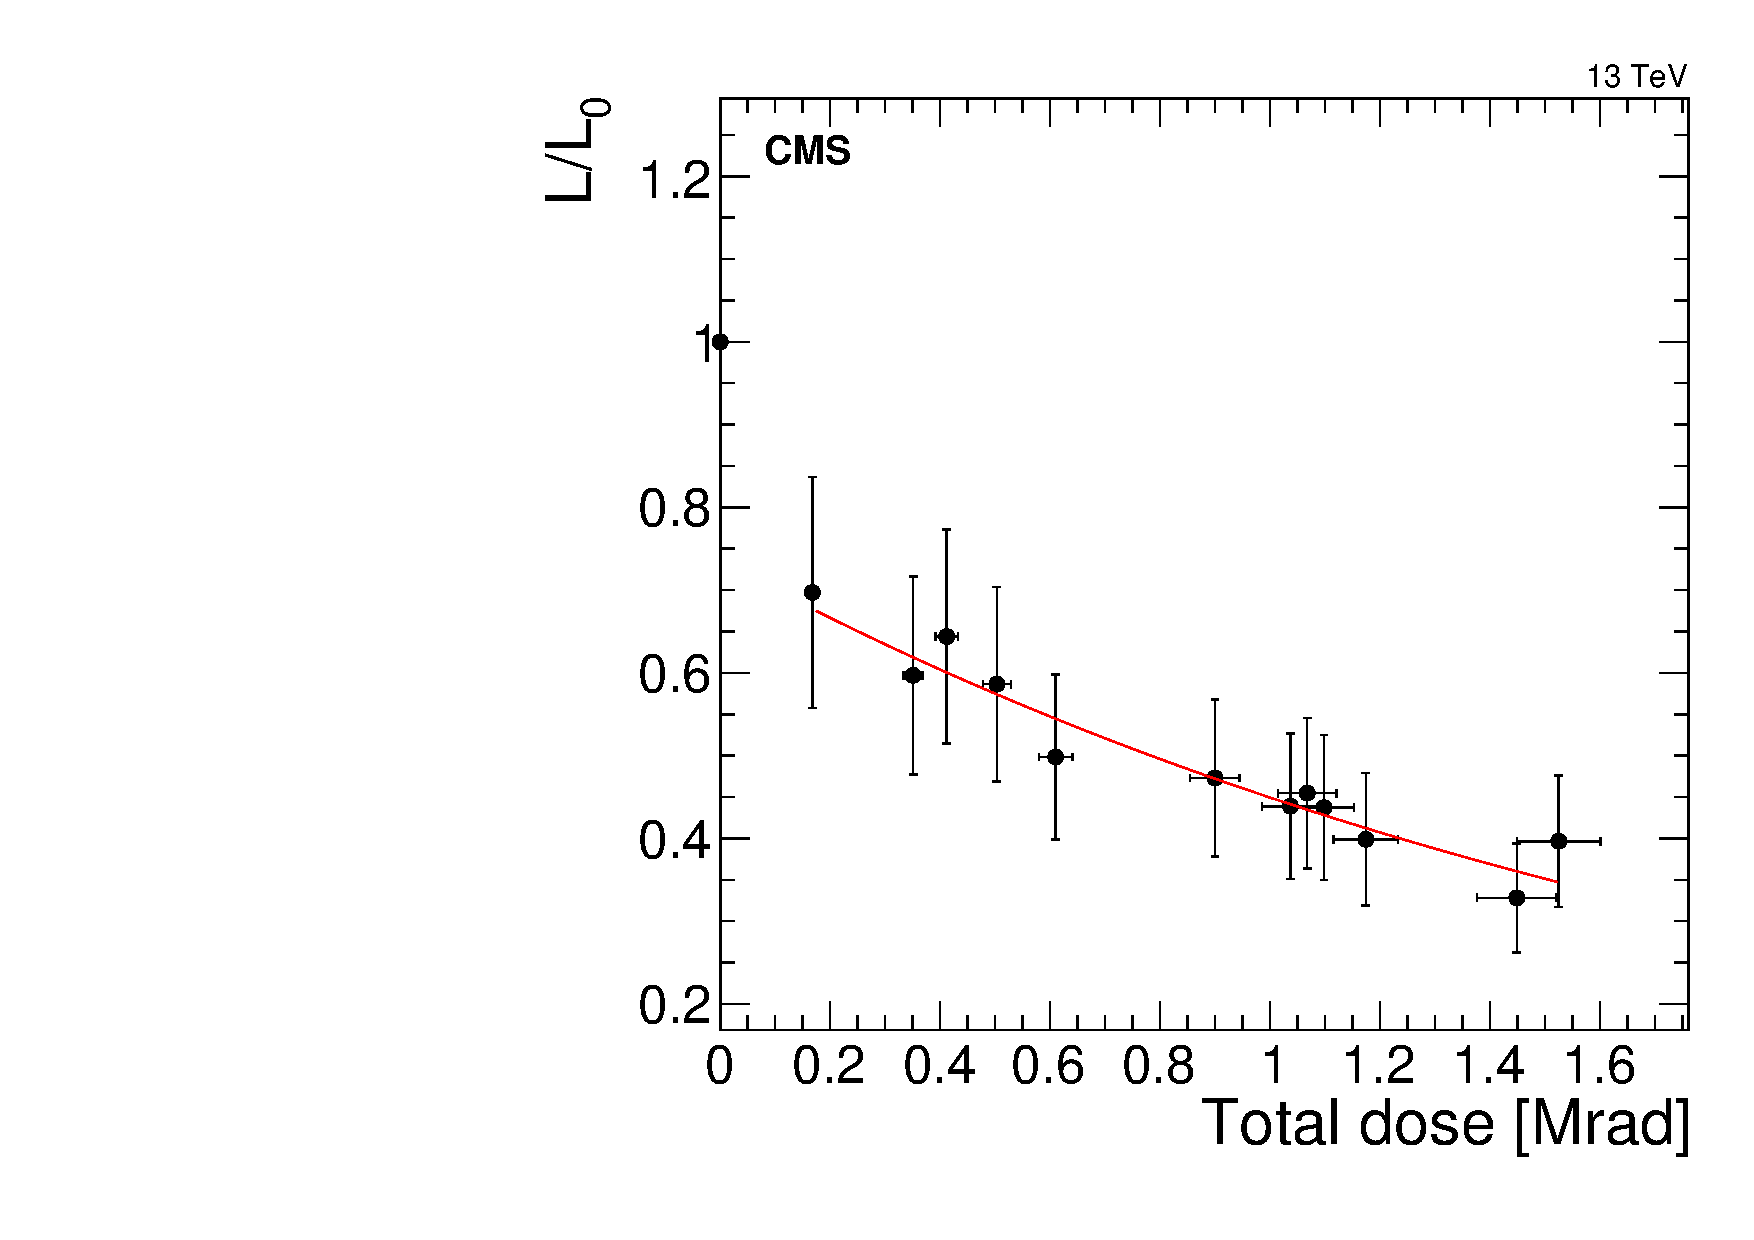
\includegraphics[width=0.45\textwidth]{figures/SCSN81-S-25p9cm-f16ch1-dose.pdf}
\caption{Relative yield versus integrated dose for SCSN81 sigma tiles at 25.9 cm from the CMS beam pipe, receiving 4.20 krad/hr. The exponential decay curve fitted to the steady-state region of light loss is shown in red.}
\label{fig:SCSN81-S-25p9cm-dose}
\end{figure} 

\begin{figure}[tbp!]
\centering
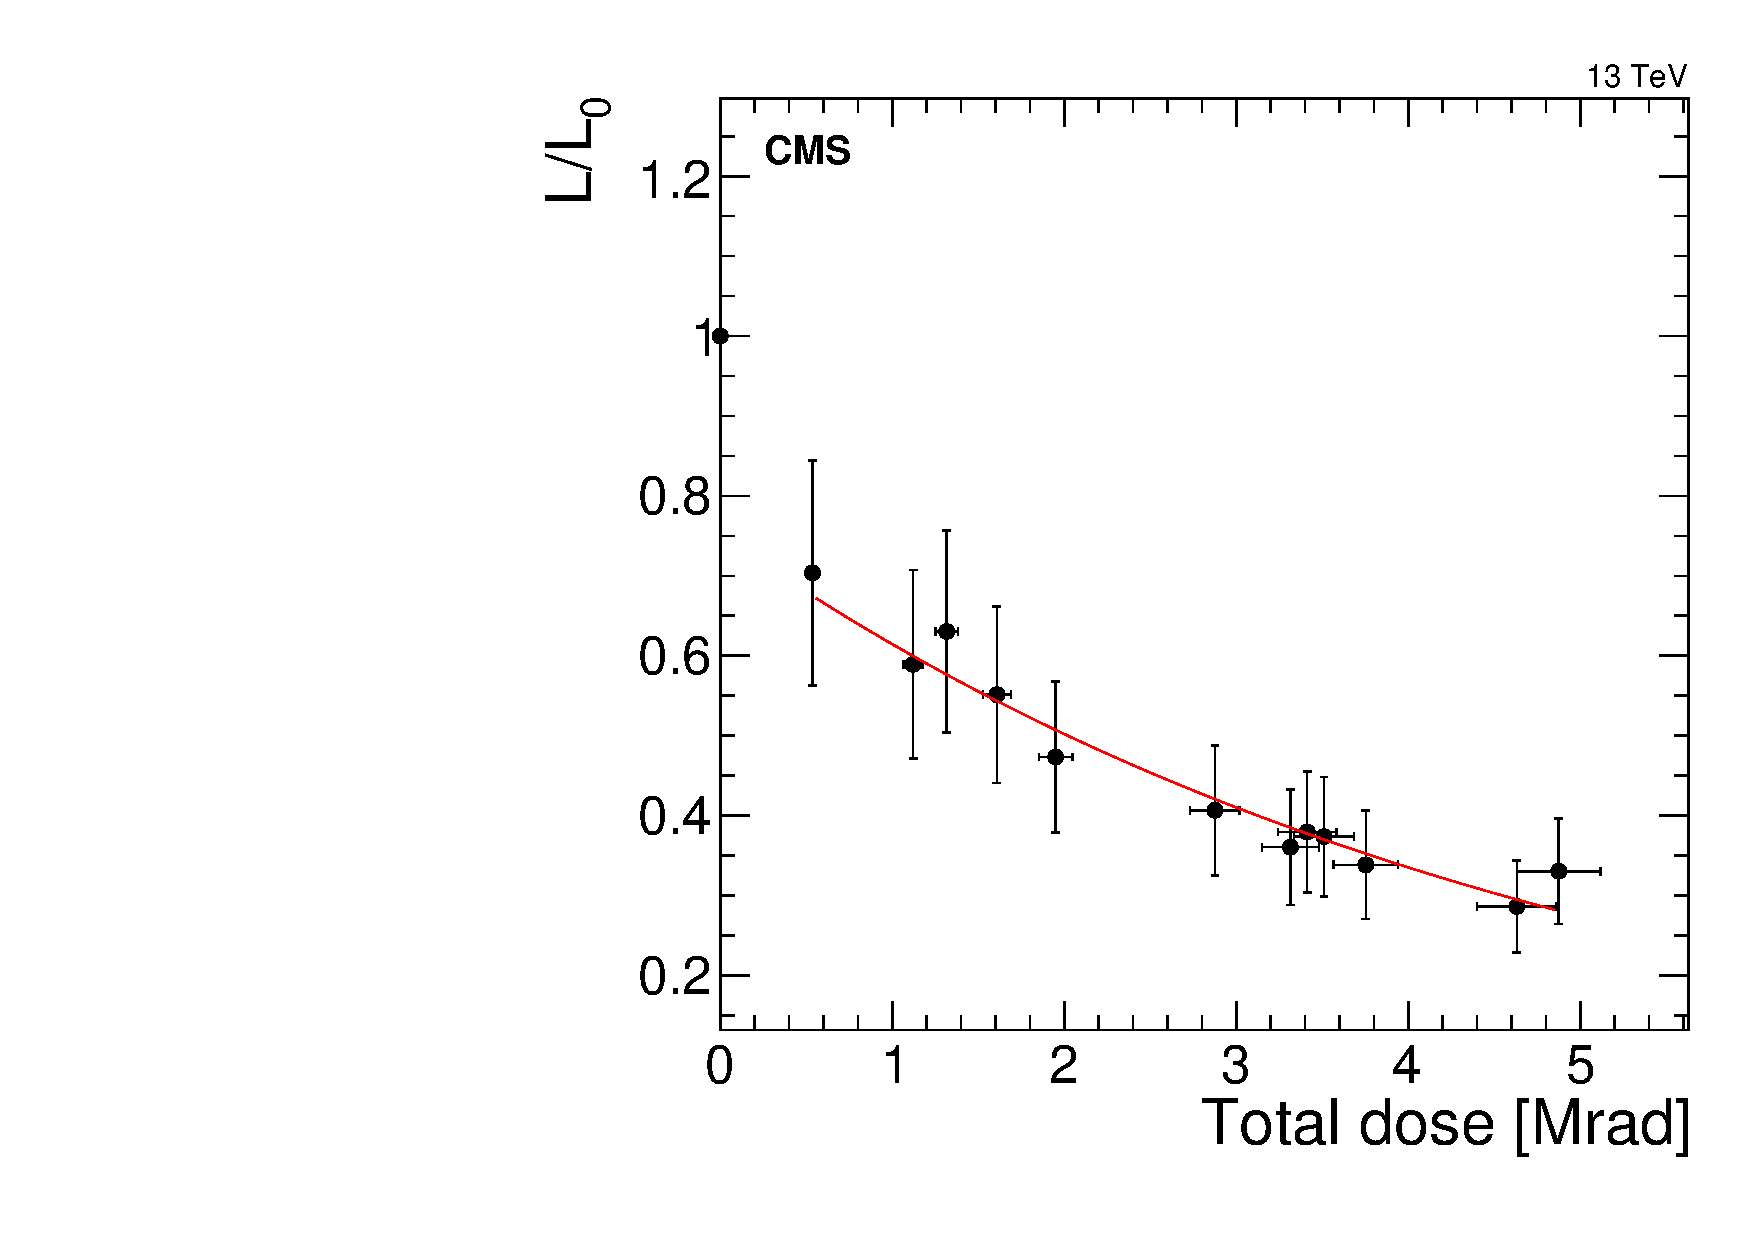
\includegraphics[width=0.45\textwidth]{figures/SCSN81-F-14p4cm-f4ch3-dose.pdf}
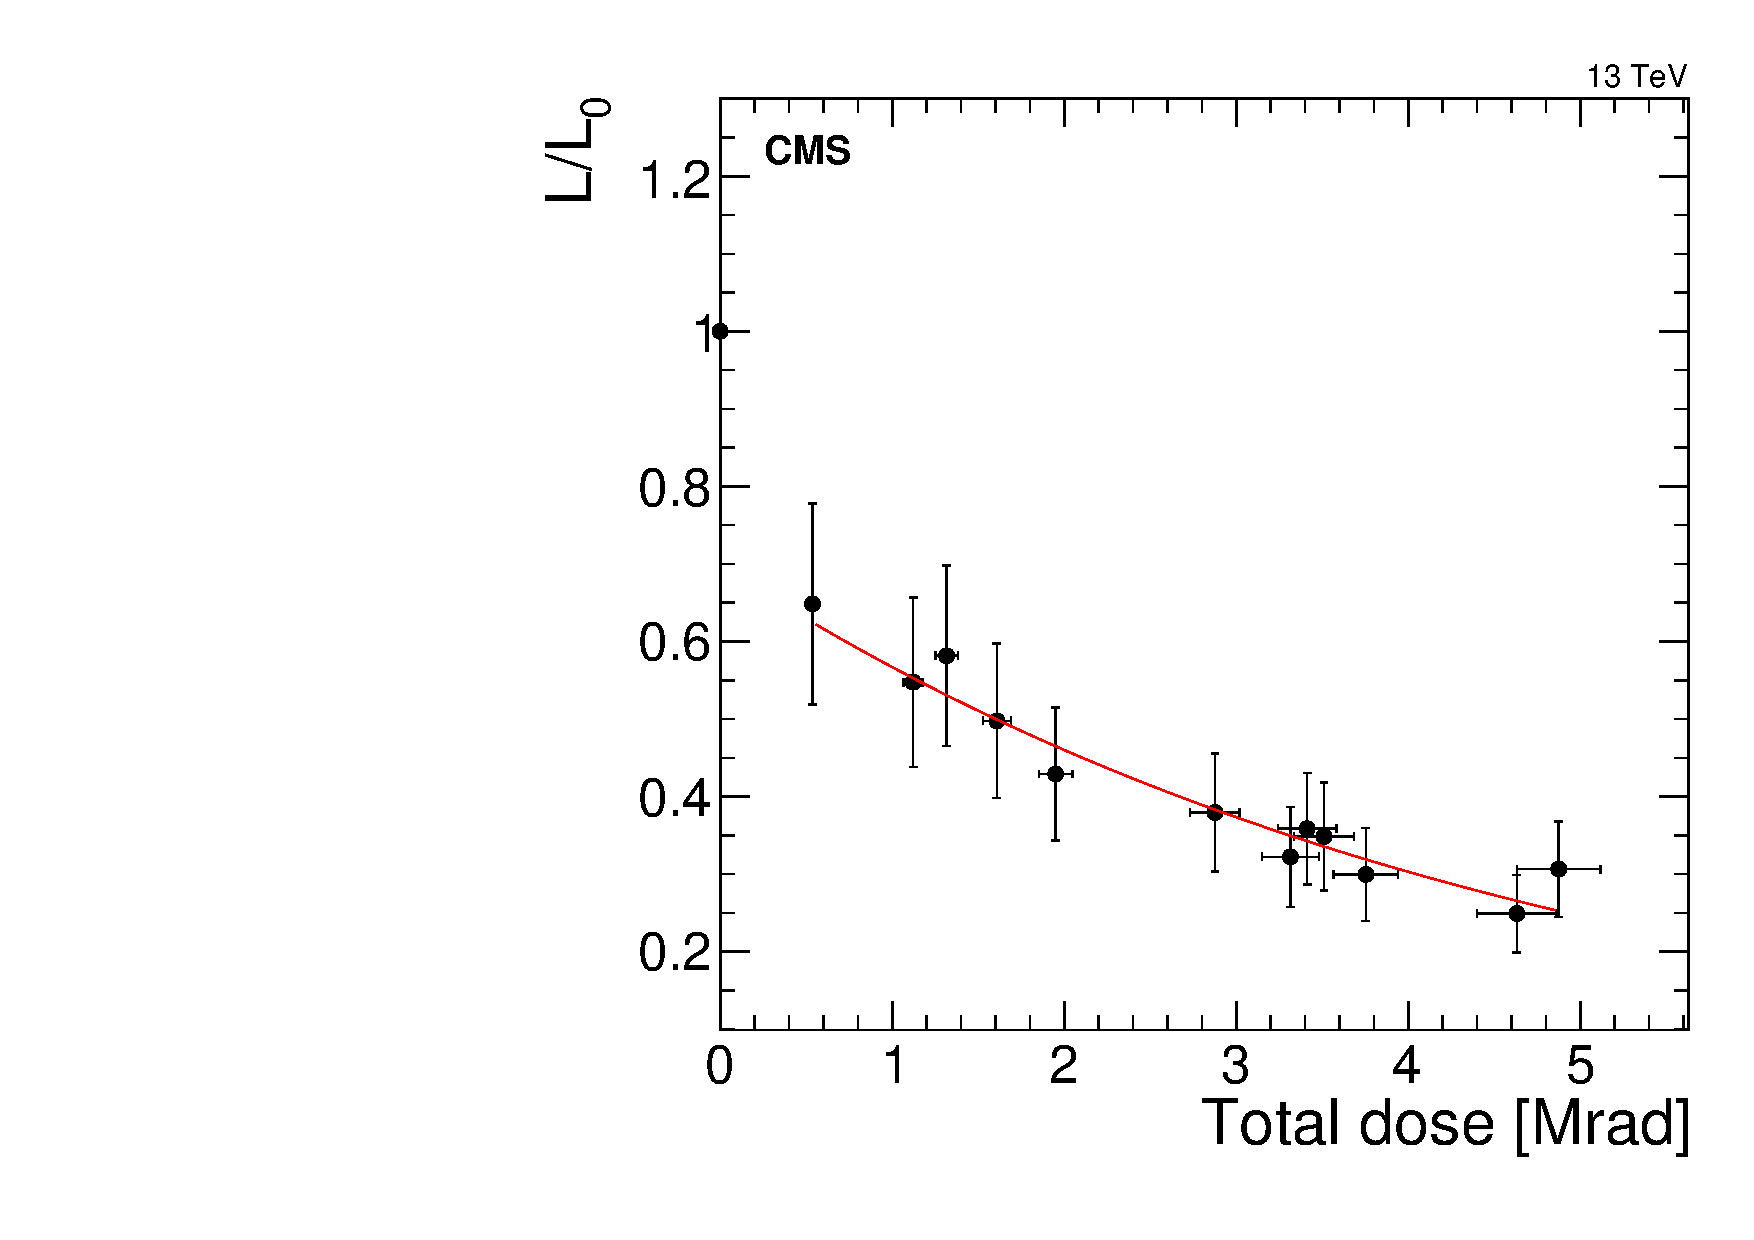
\includegraphics[width=0.45\textwidth]{figures/SCSN81-F-14p4cm-f7ch0-dose.pdf}
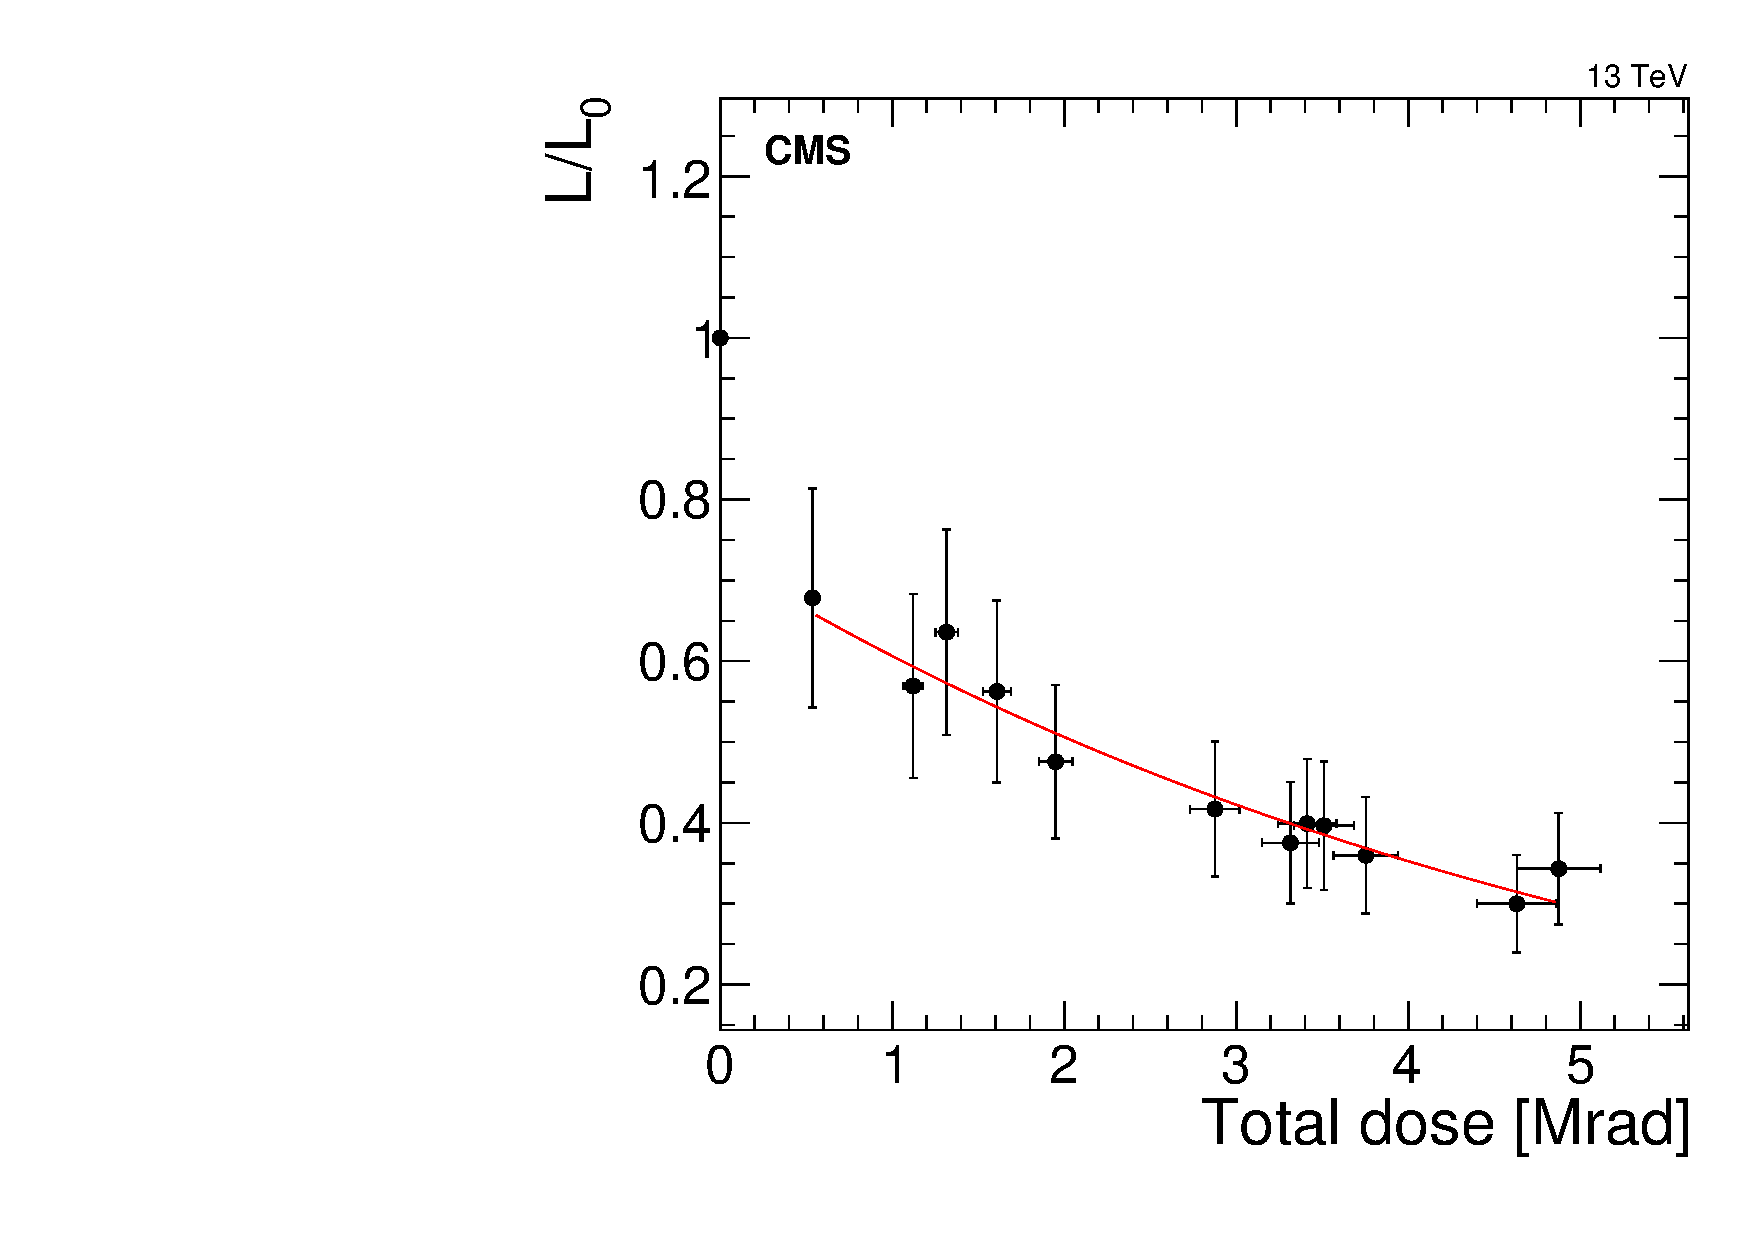
\includegraphics[width=0.45\textwidth]{figures/SCSN81-F-14p4cm-f18ch0-dose.pdf}
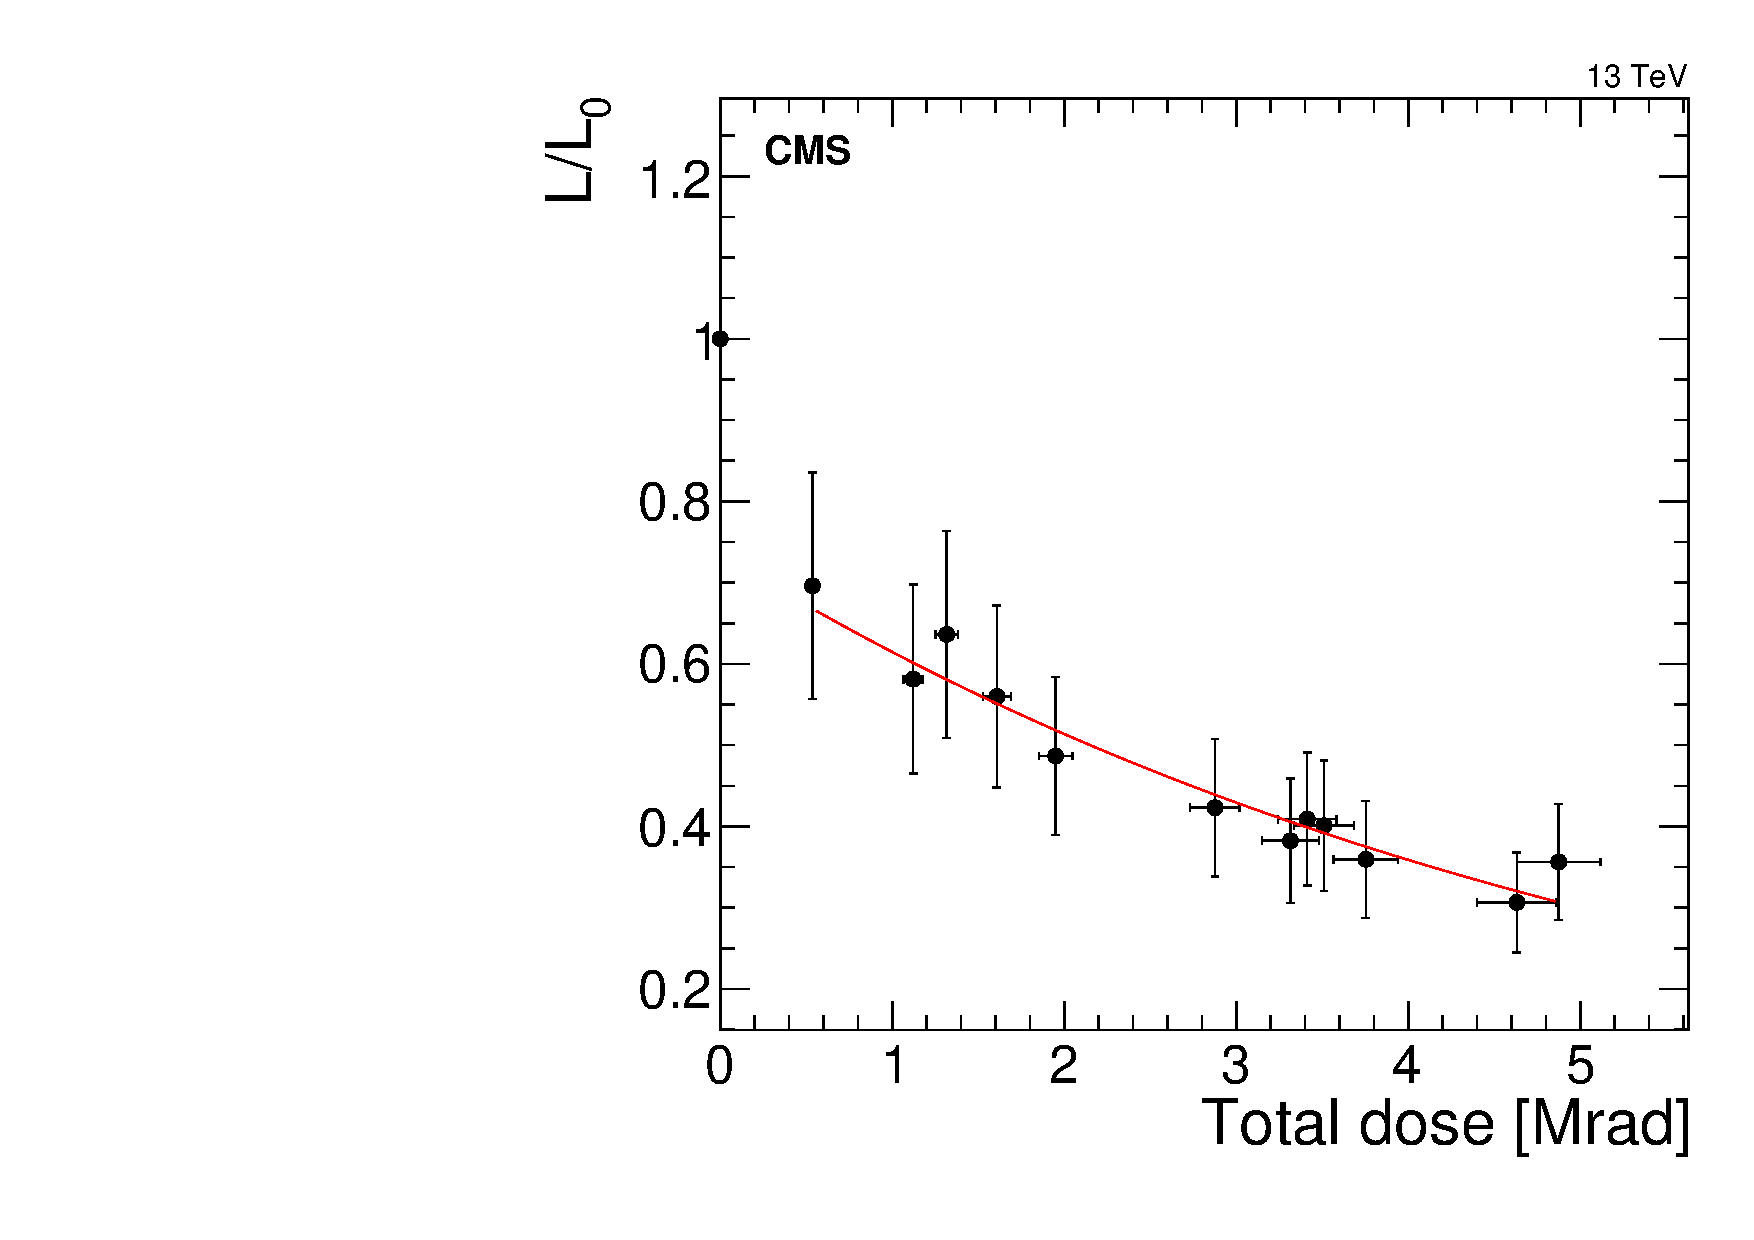
\includegraphics[width=0.45\textwidth]{figures/SCSN81-F-14p4cm-f18ch1-dose.pdf}
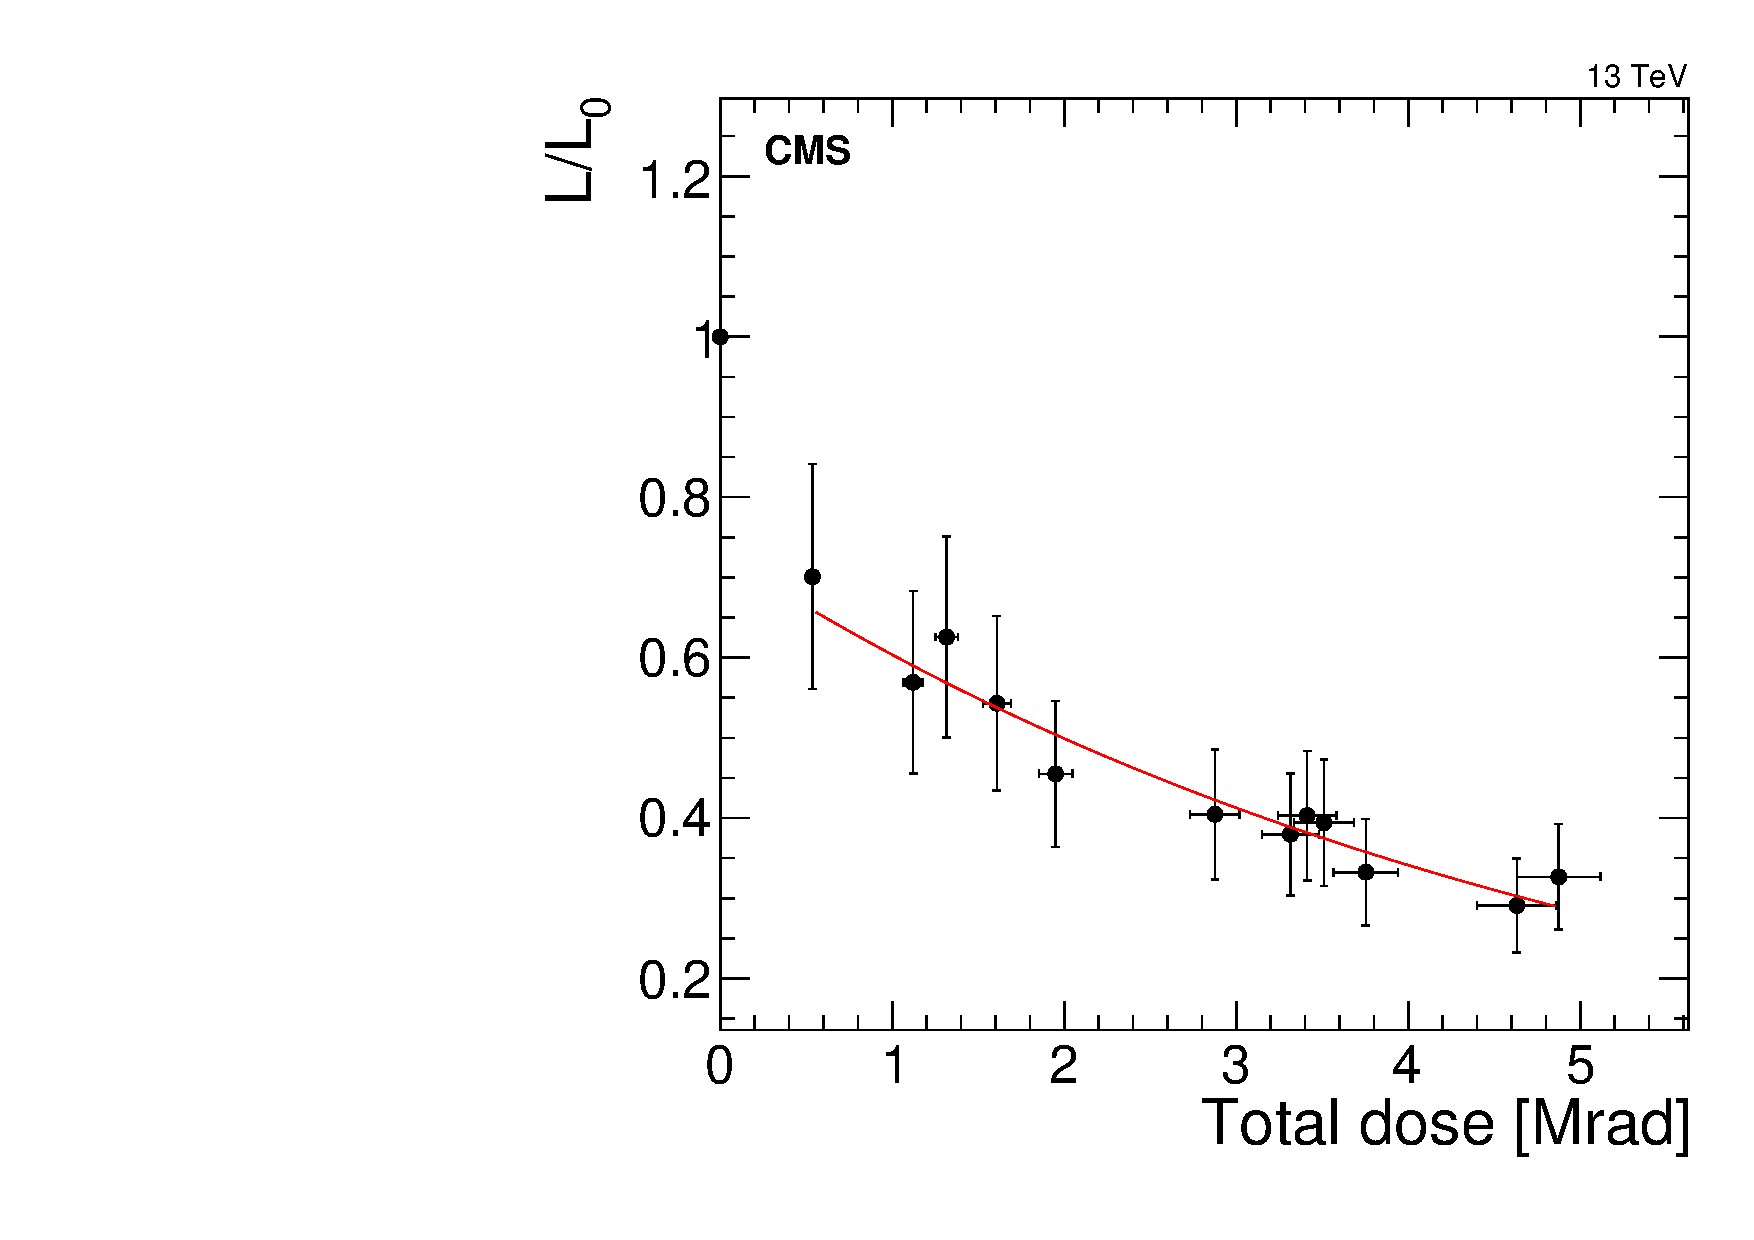
\includegraphics[width=0.45\textwidth]{figures/SCSN81-F-14p4cm-f18ch2-dose.pdf}
\caption{Relative yield versus integrated dose for SCSN81 finger tiles at 14.4 cm from the CMS beam pipe, receiving 13.44 krad/hr. The exponential decay curve fitted to the steady-state region of light loss is shown in red.}
\label{fig:SCSN81-F-14p4cm-dose}
\end{figure} 

\begin{figure}[tbp!]
\centering
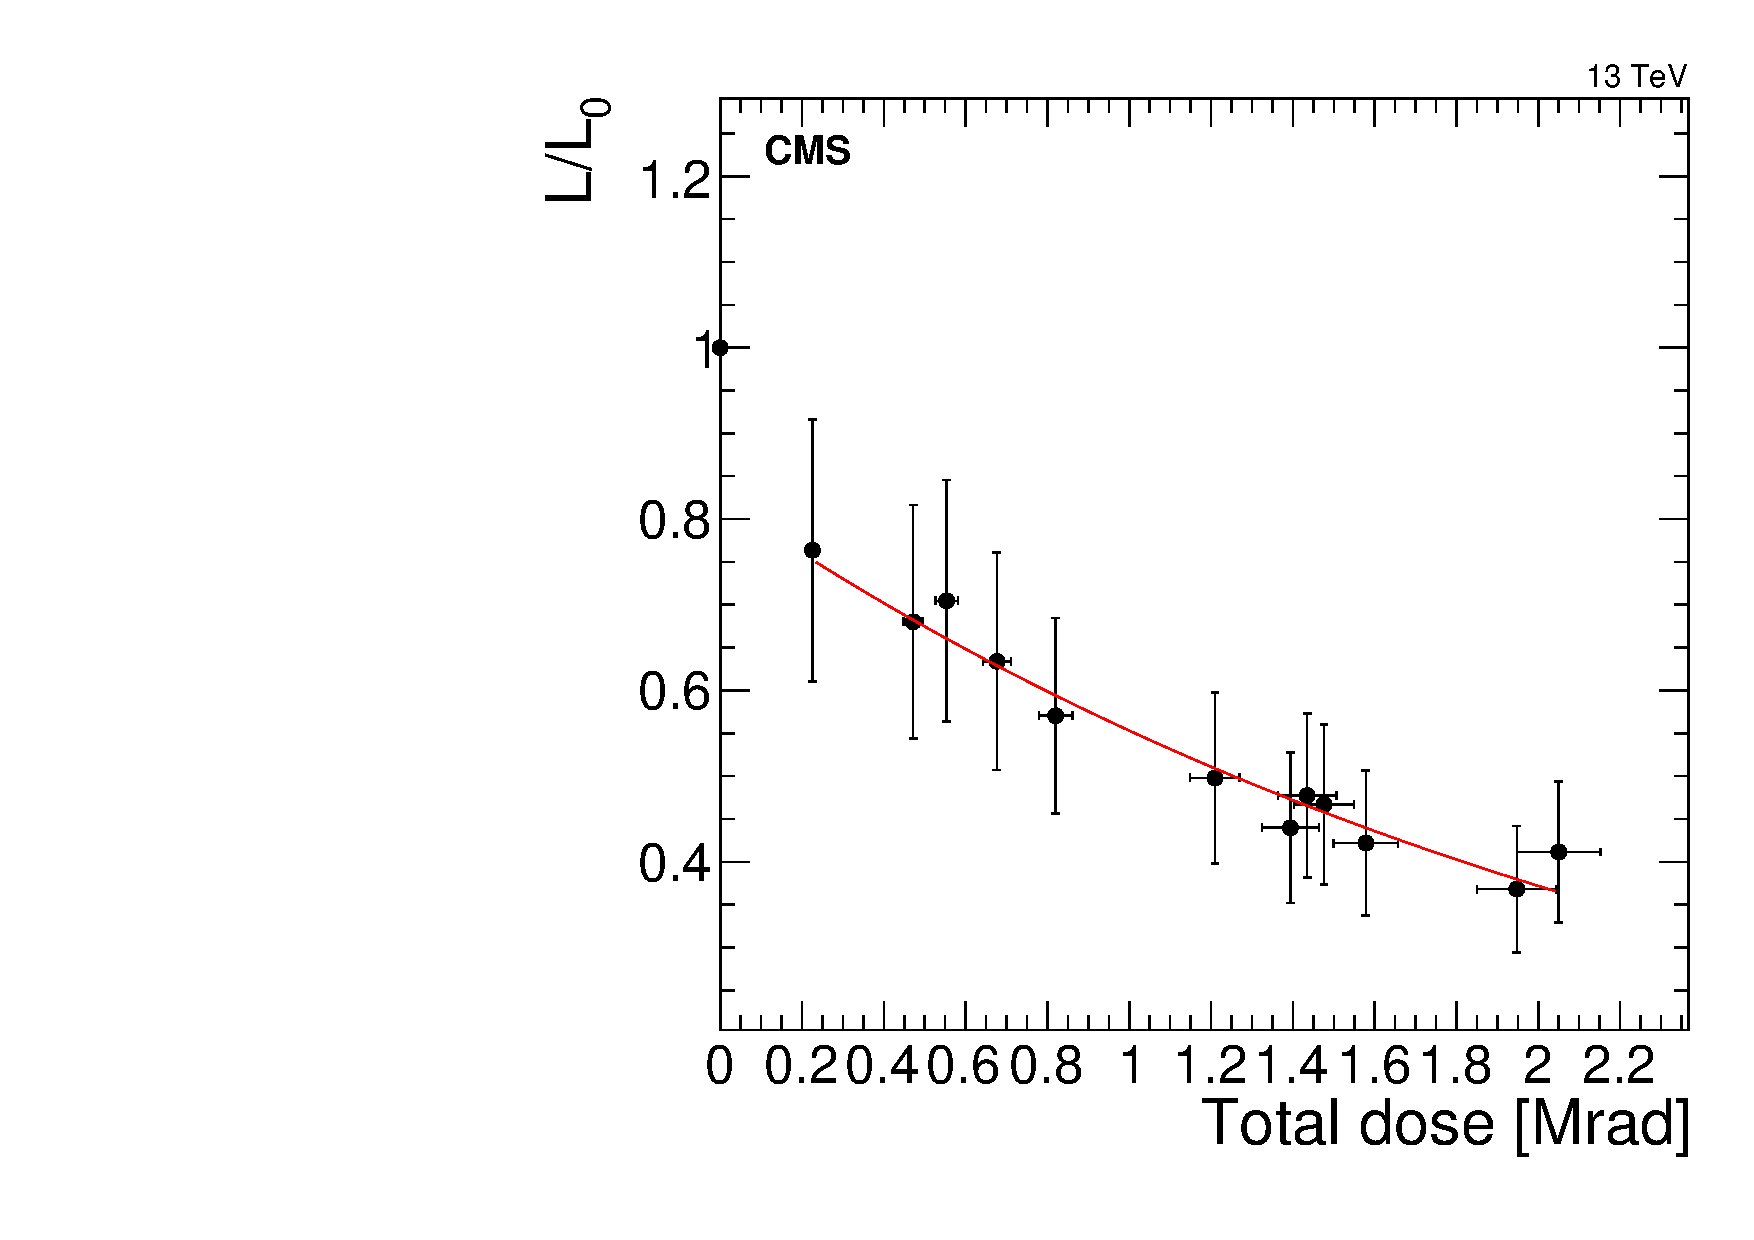
\includegraphics[width=0.45\textwidth]{figures/SCSN81-F-20p8cm-f2ch0-dose.pdf}
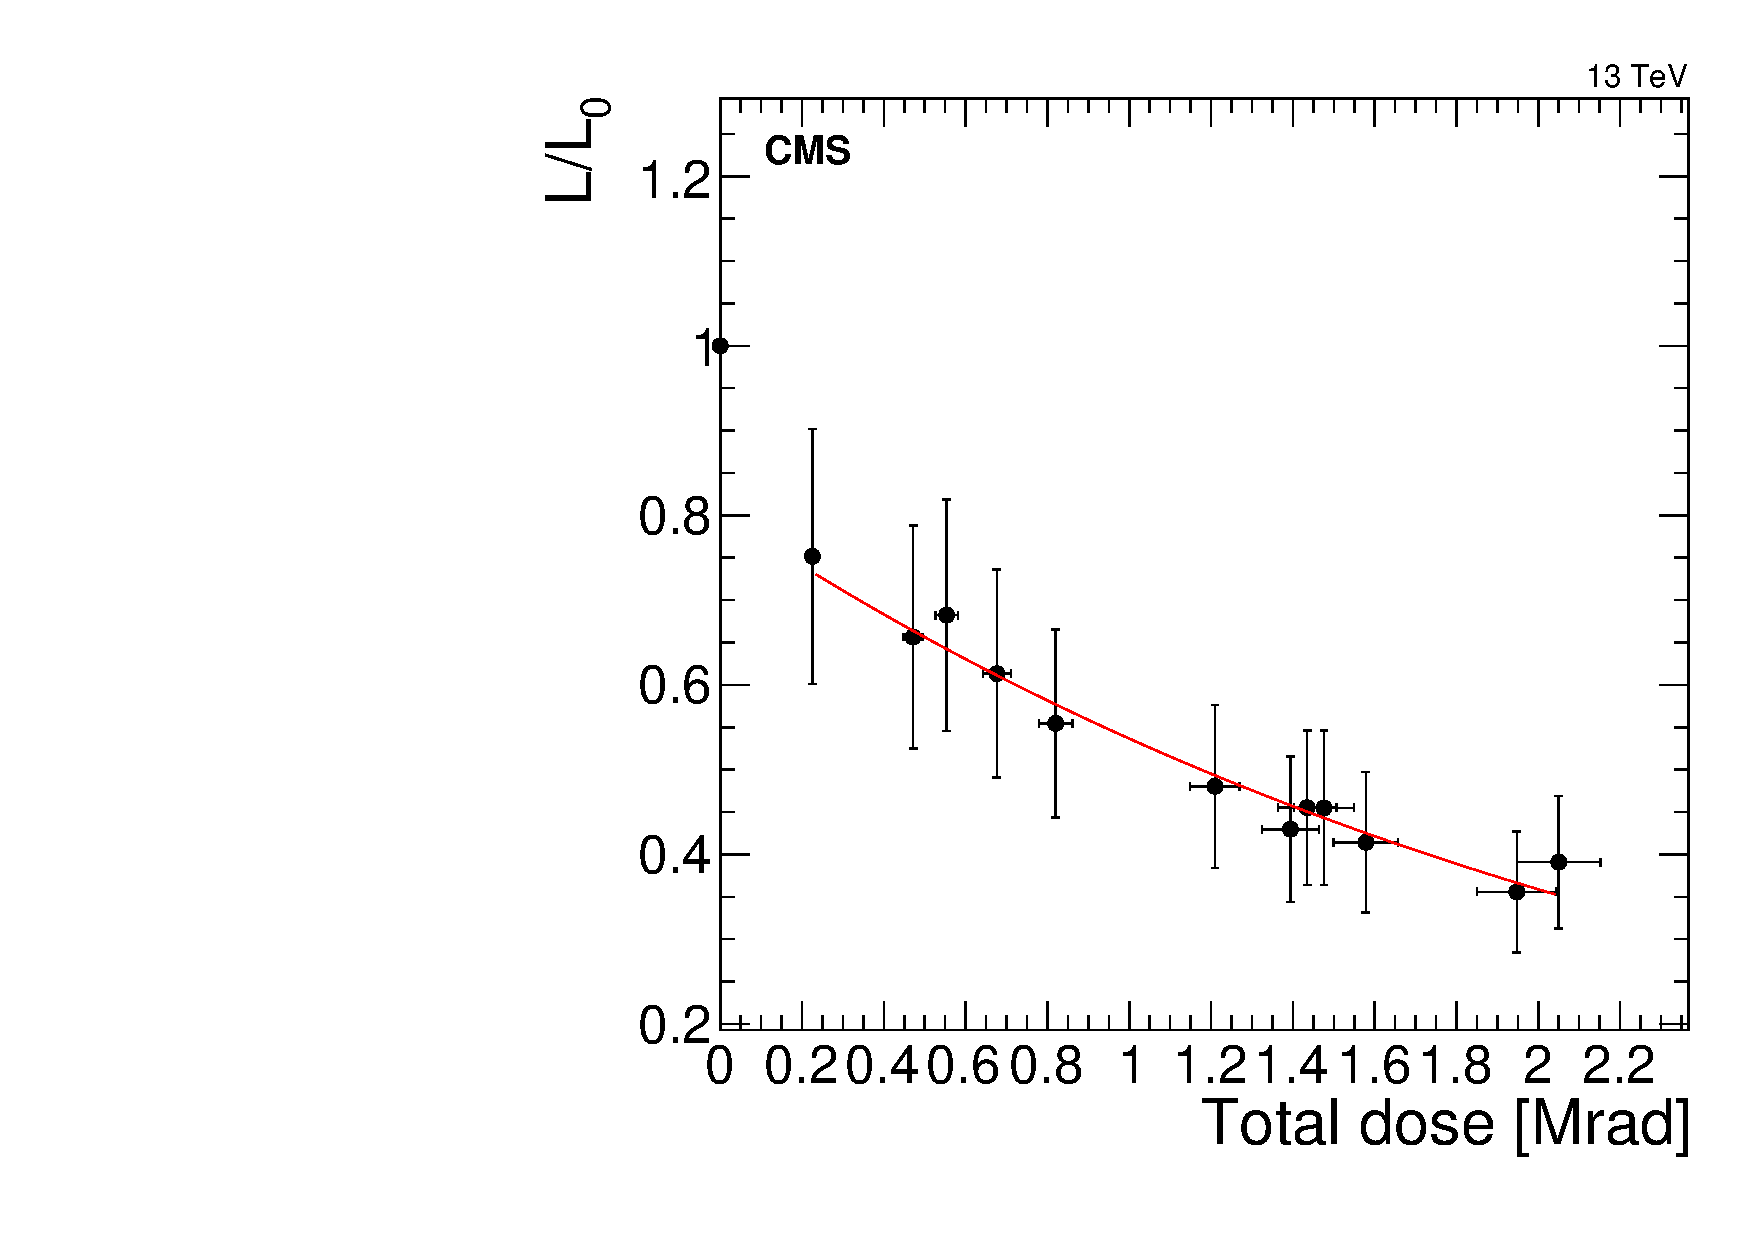
\includegraphics[width=0.45\textwidth]{figures/SCSN81-F-20p8cm-f4ch1-dose.pdf}
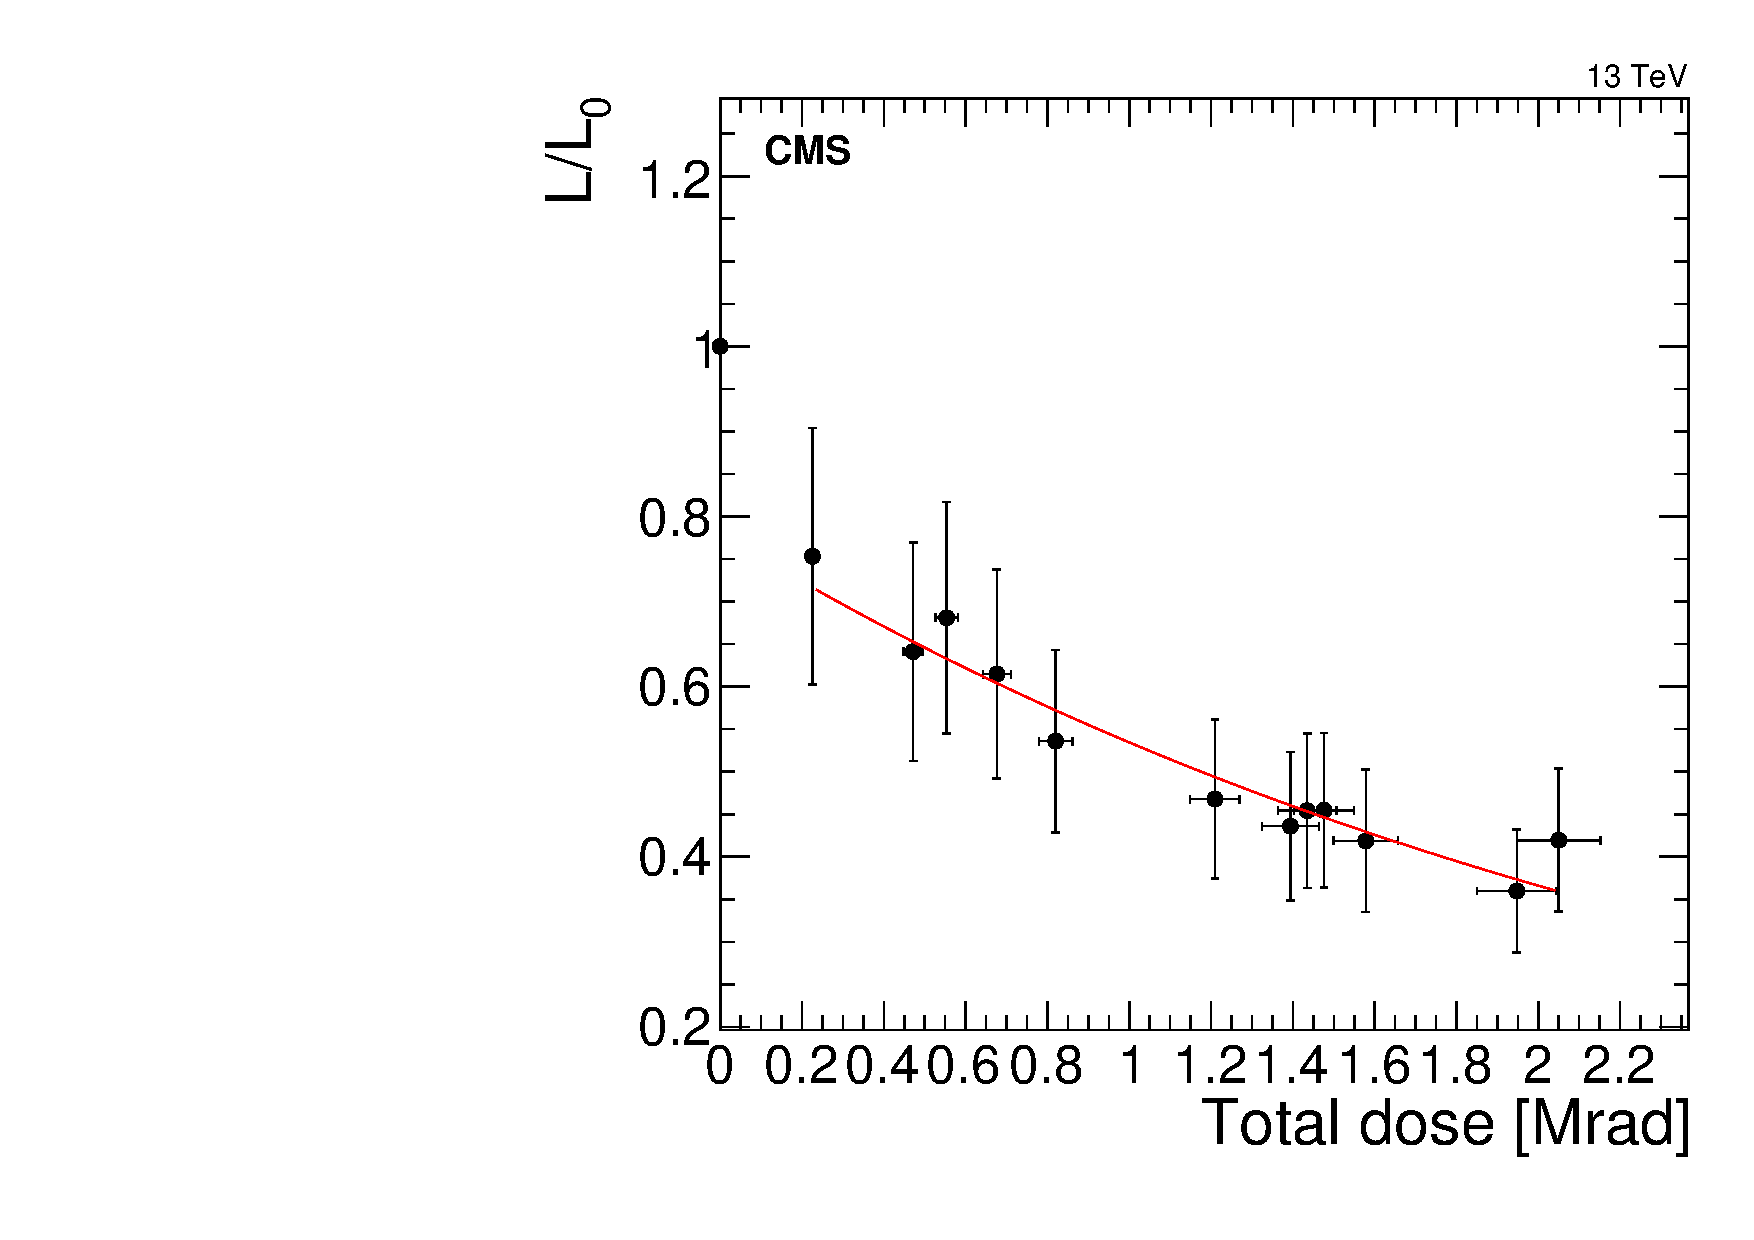
\includegraphics[width=0.45\textwidth]{figures/SCSN81-F-20p8cm-f15ch2-dose.pdf}
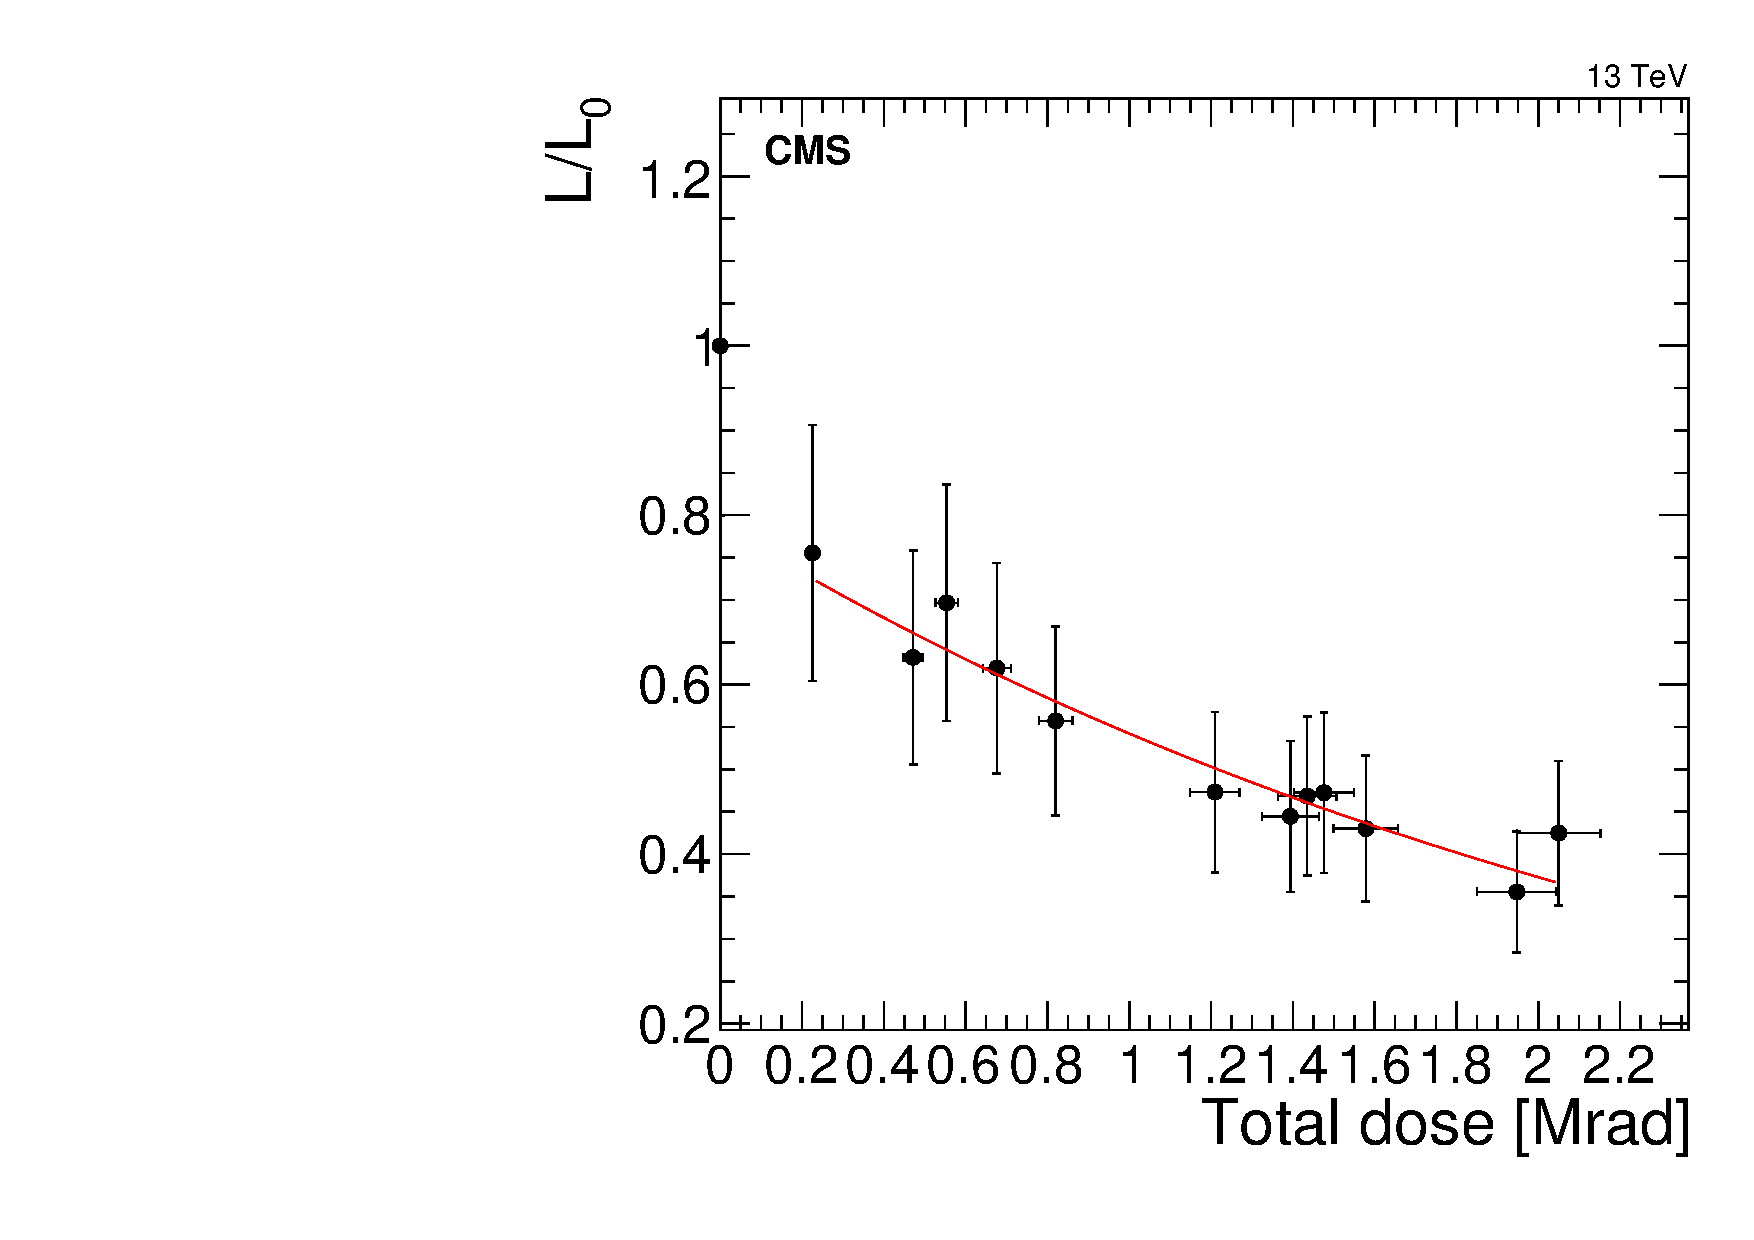
\includegraphics[width=0.45\textwidth]{figures/SCSN81-F-20p8cm-f15ch3-dose.pdf}
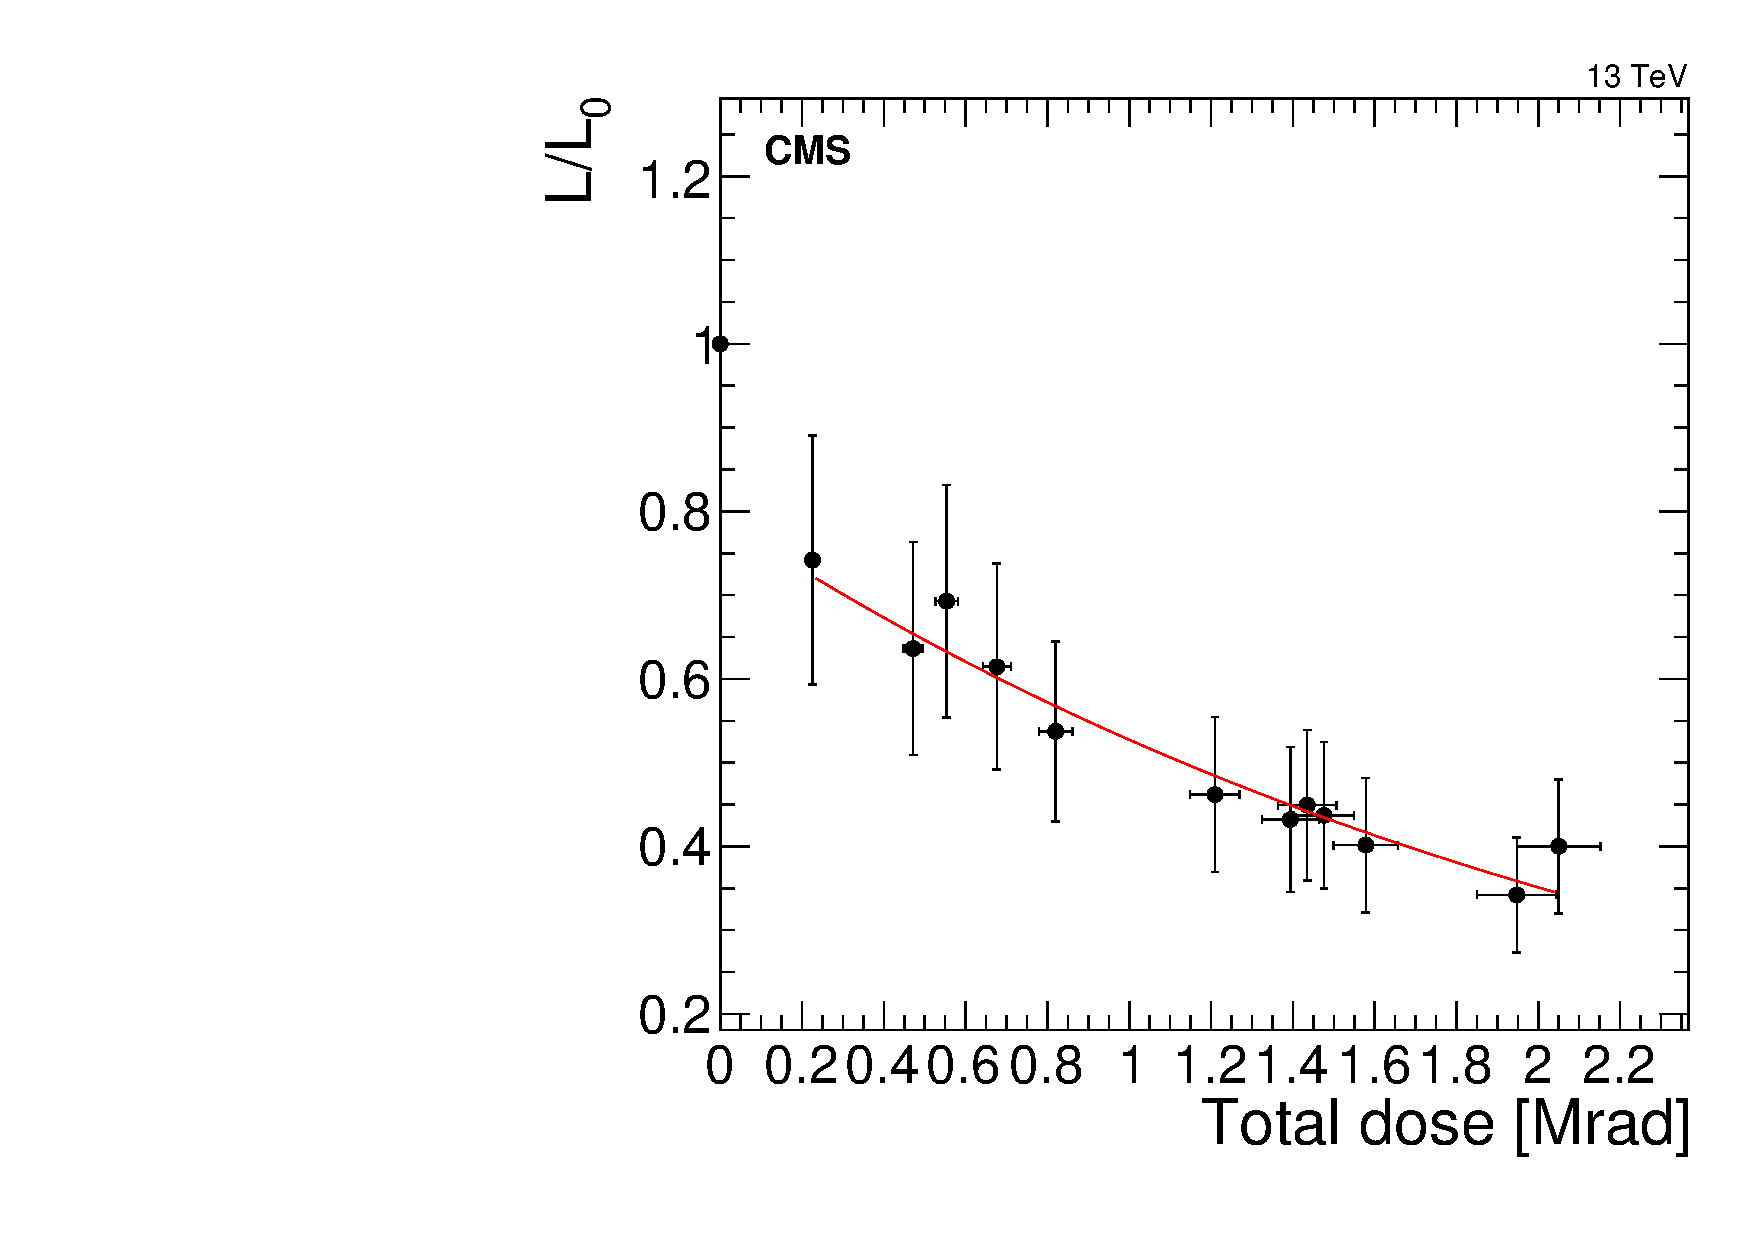
\includegraphics[width=0.45\textwidth]{figures/SCSN81-F-20p8cm-f20ch2-dose.pdf}
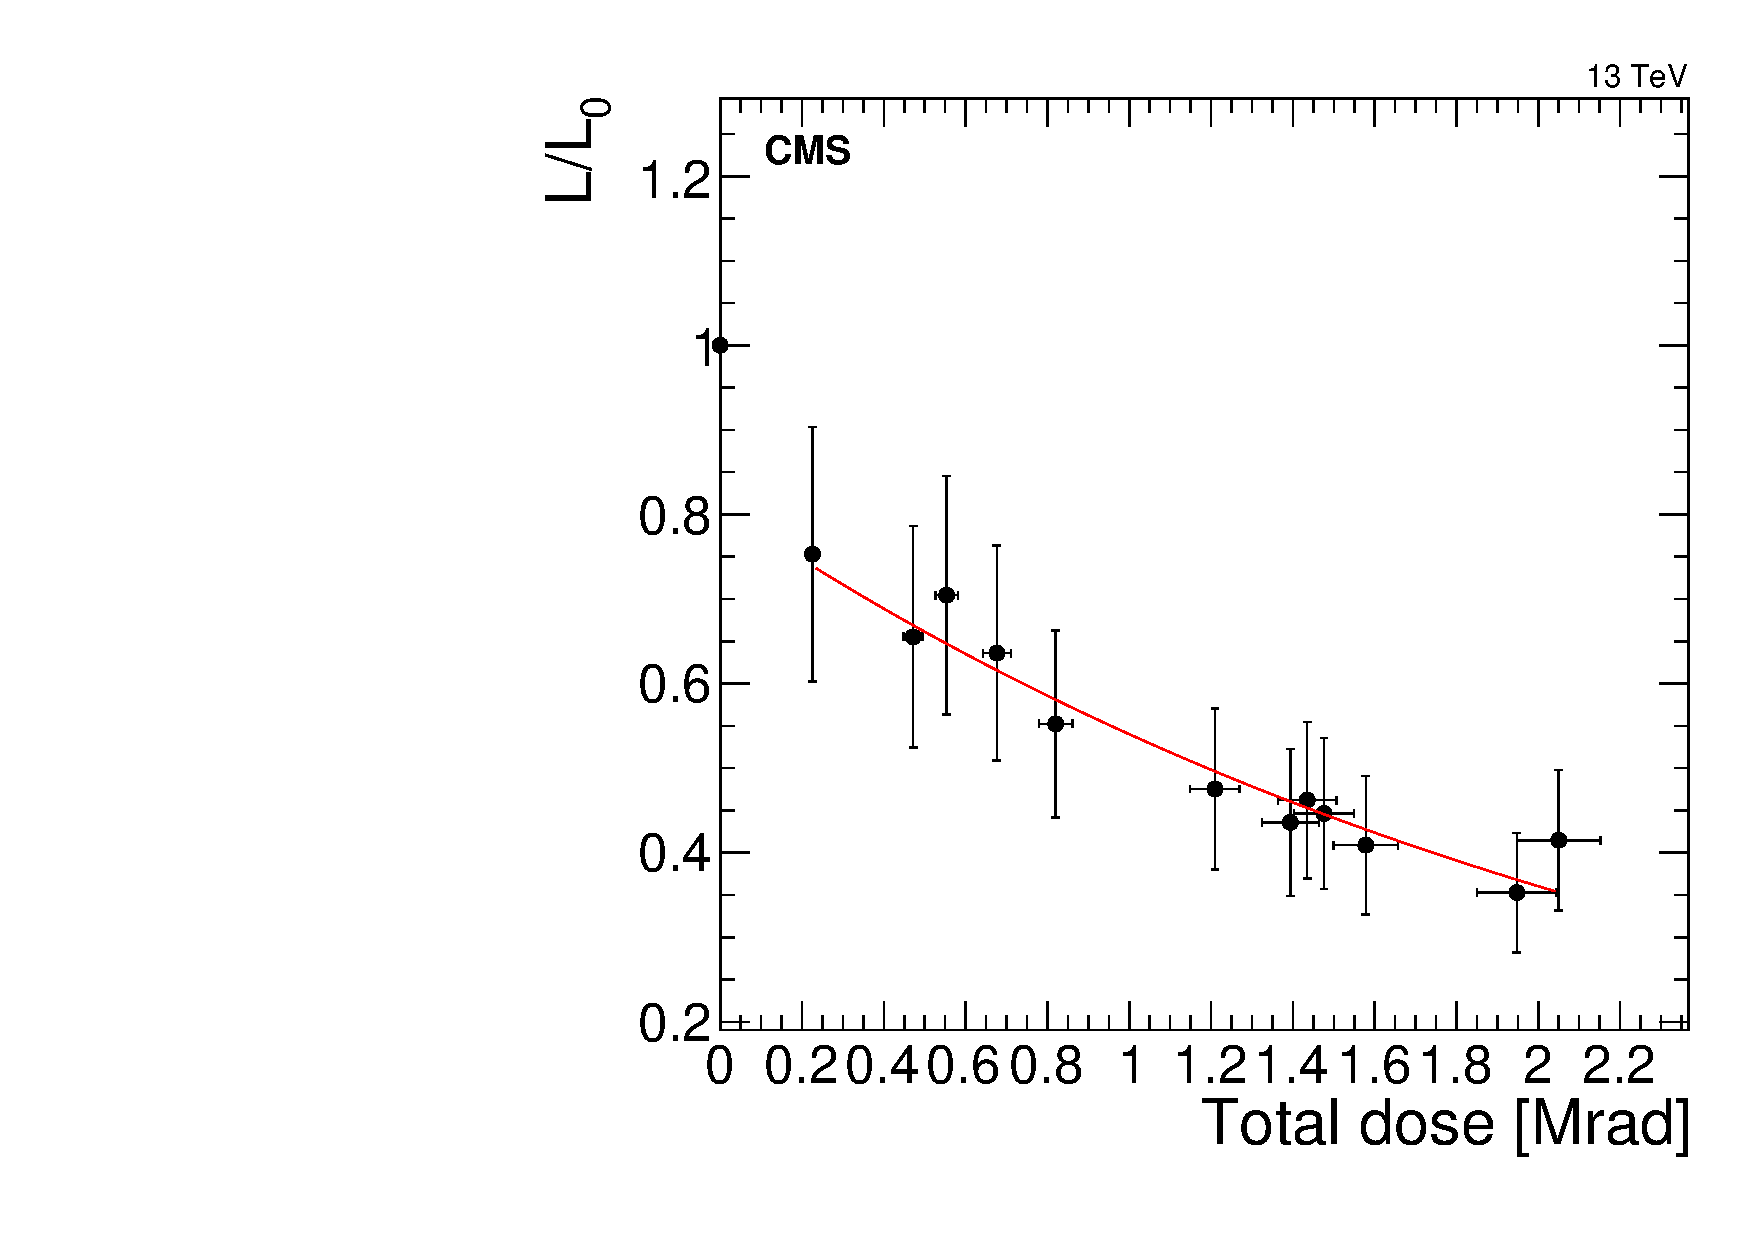
\includegraphics[width=0.45\textwidth]{figures/SCSN81-F-20p8cm-f20ch3-dose.pdf}
\caption{Relative yield versus integrated dose for SCSN81 finger tiles at 20.8 cm from the CMS beam pipe, receiving 5.65 krad/hr. The exponential decay curve fitted to the steady-state region of light loss is shown in red.}
\label{fig:SCSN81-F-20p8cm-dose}
\end{figure} 

\begin{figure}[tbp!]
\centering
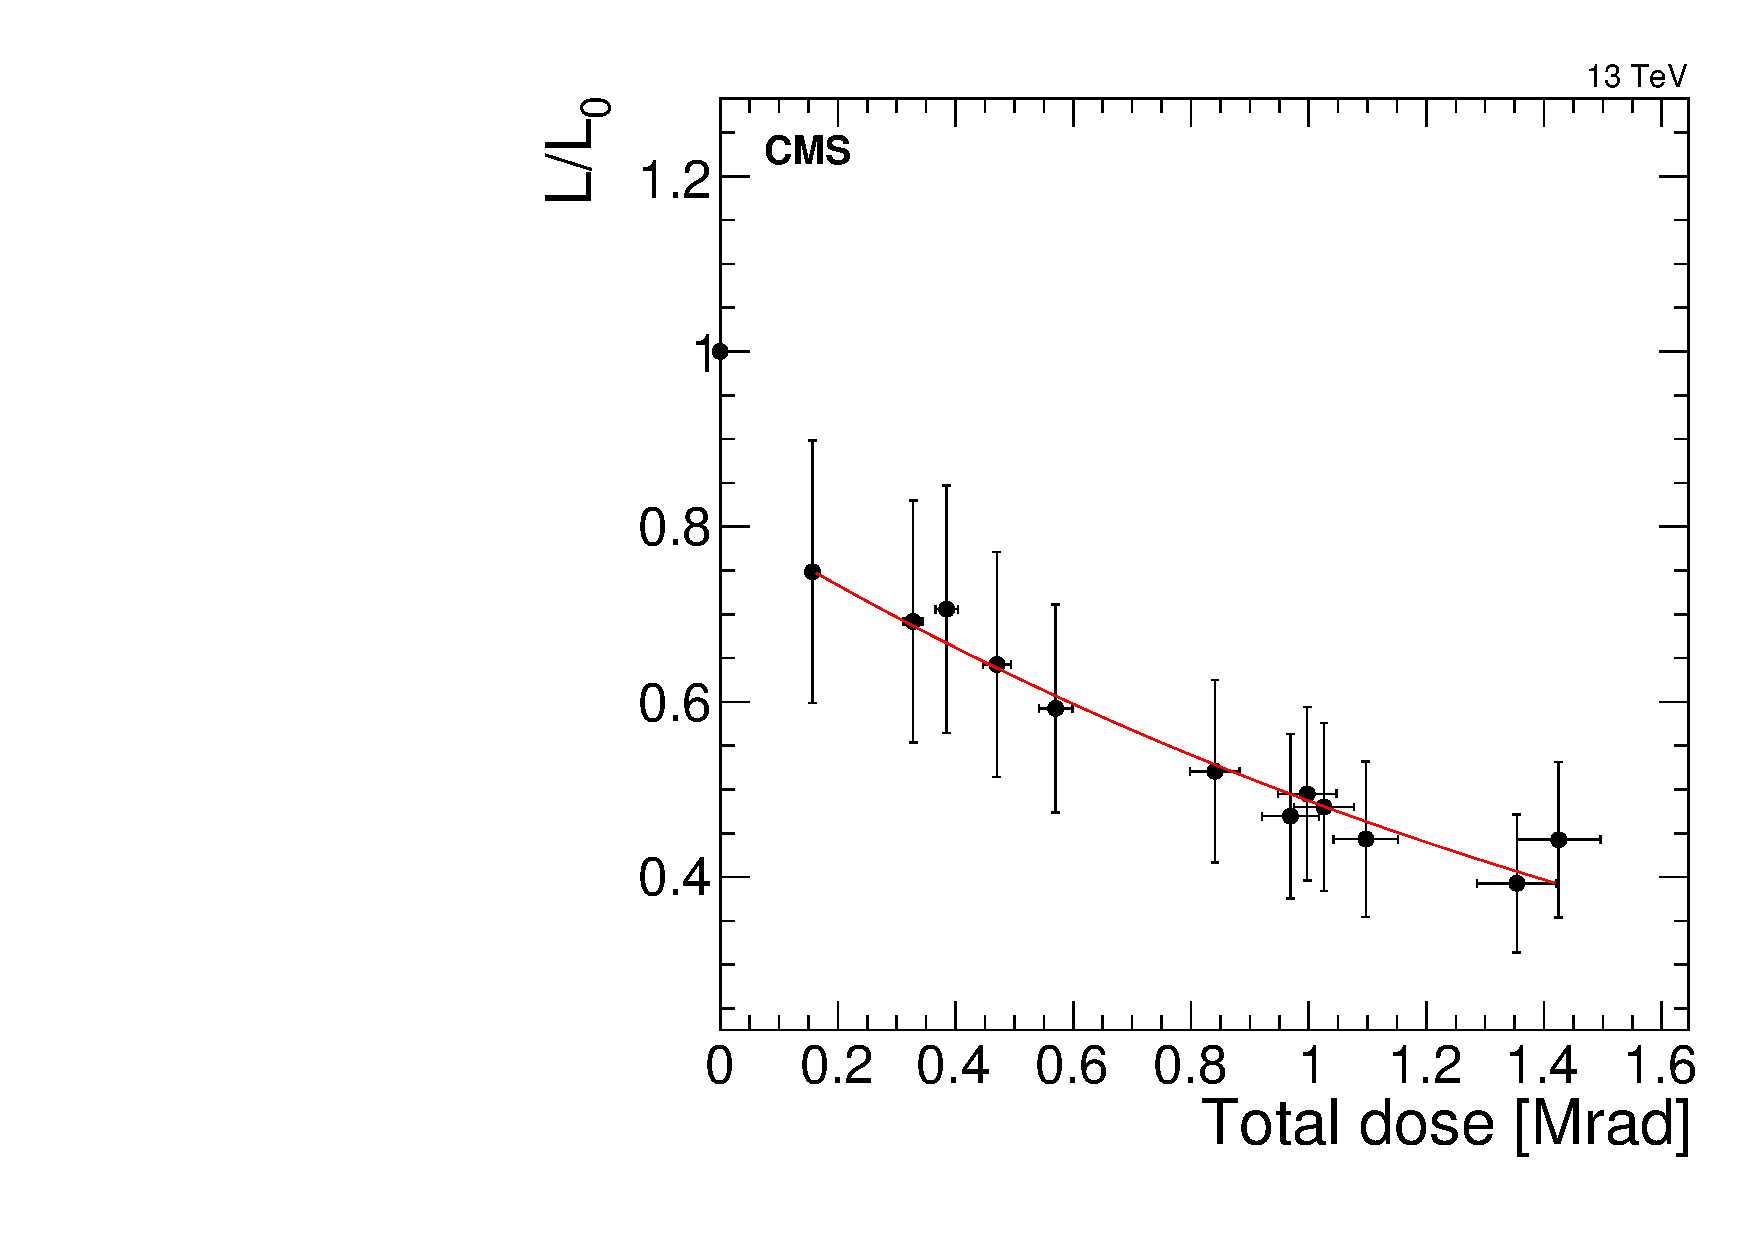
\includegraphics[width=0.32\textwidth]{figures/SCSN81-F-27p2cm-f2ch5-dose.pdf}
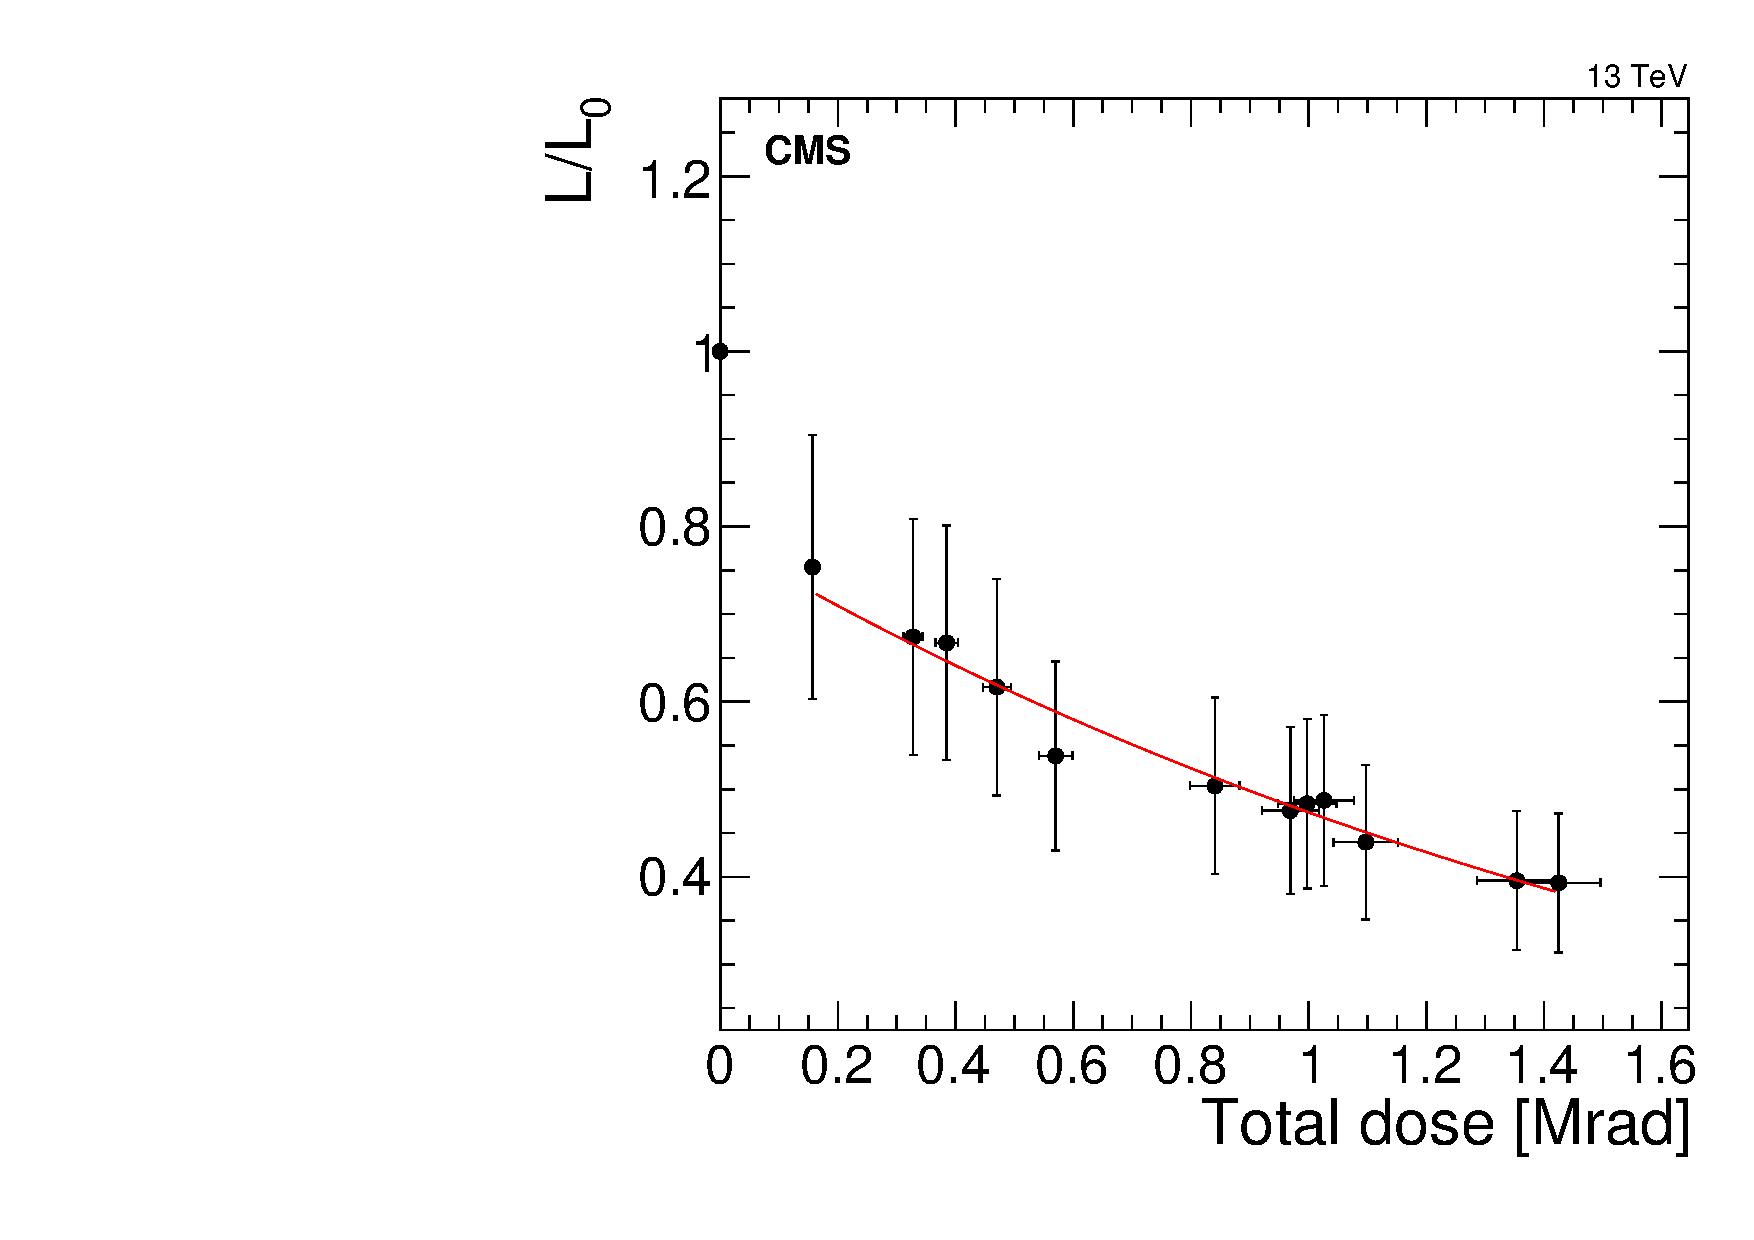
\includegraphics[width=0.32\textwidth]{figures/SCSN81-F-27p2cm-f3ch5-dose.pdf}
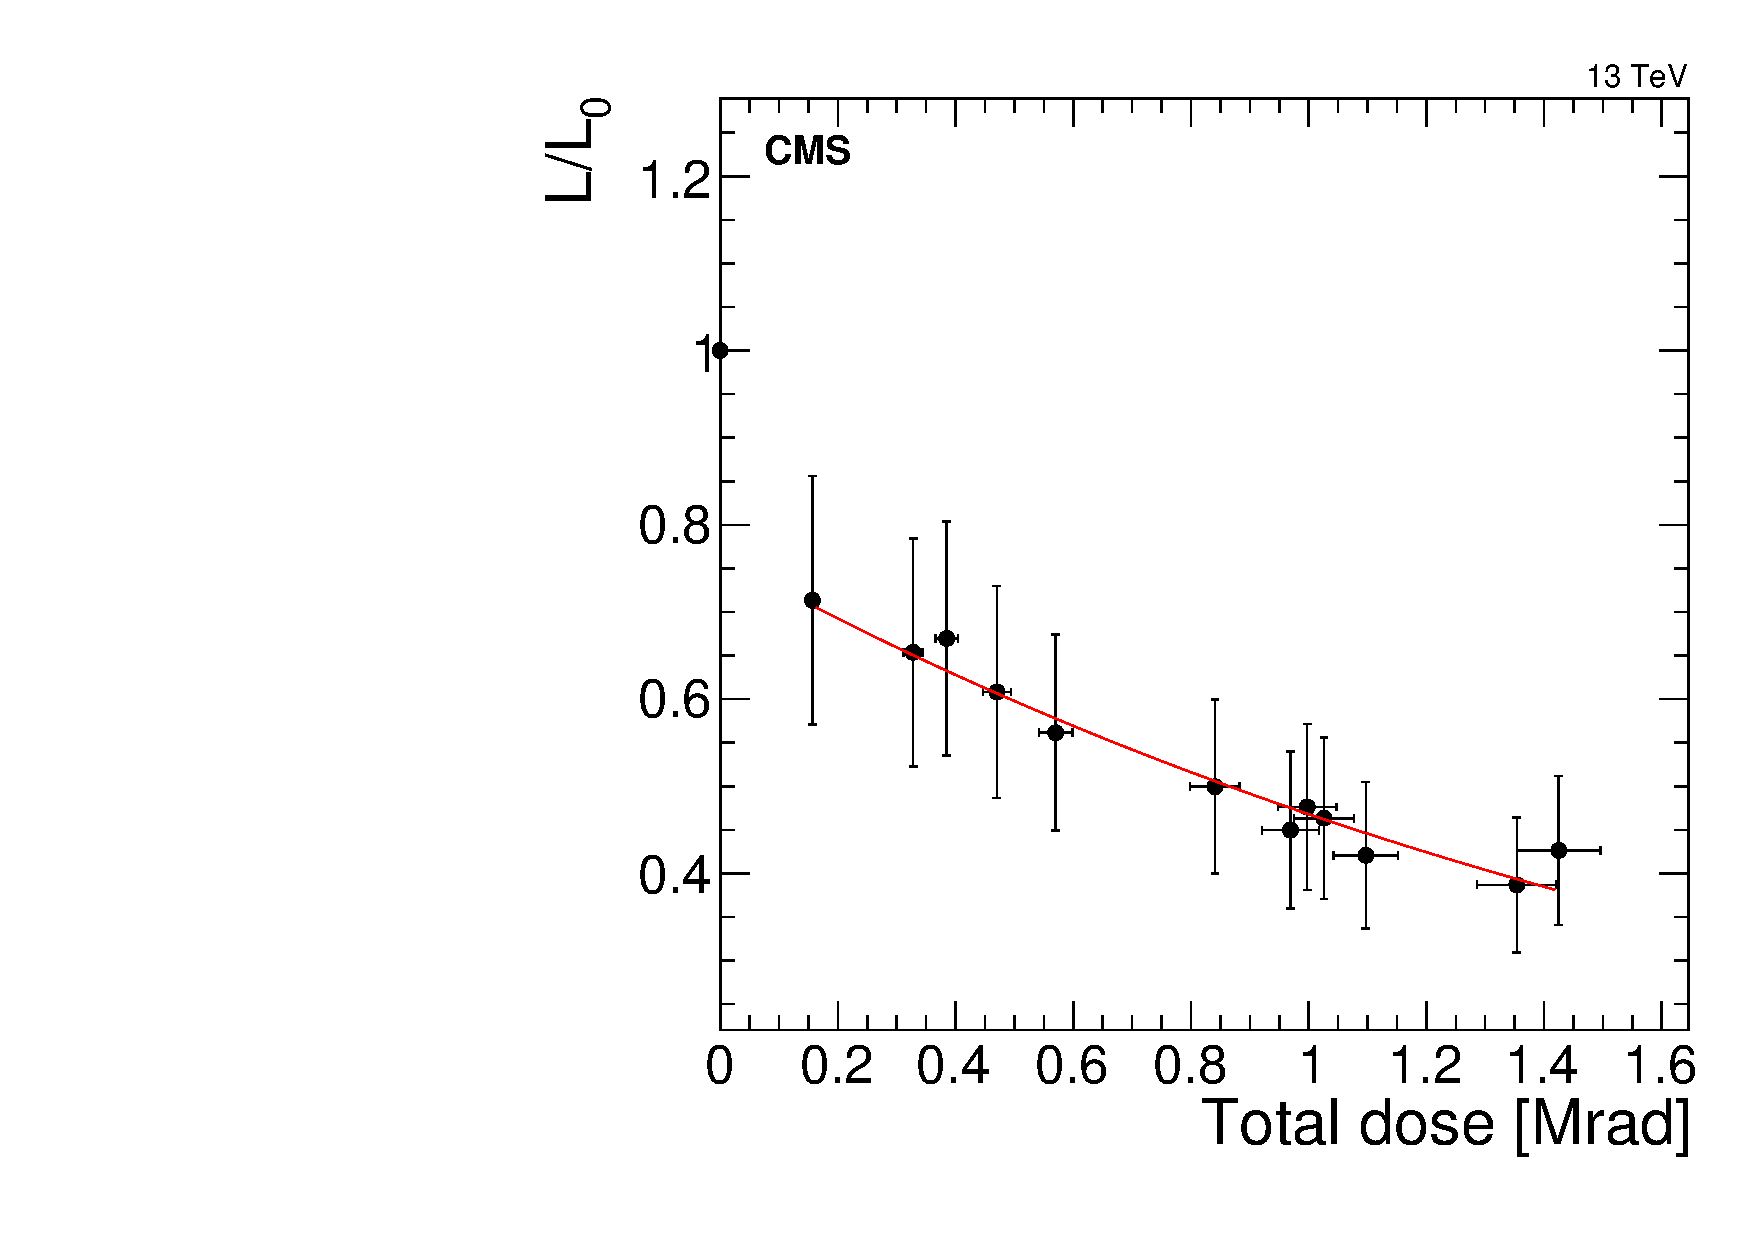
\includegraphics[width=0.32\textwidth]{figures/SCSN81-F-27p2cm-f4ch0-dose.pdf}
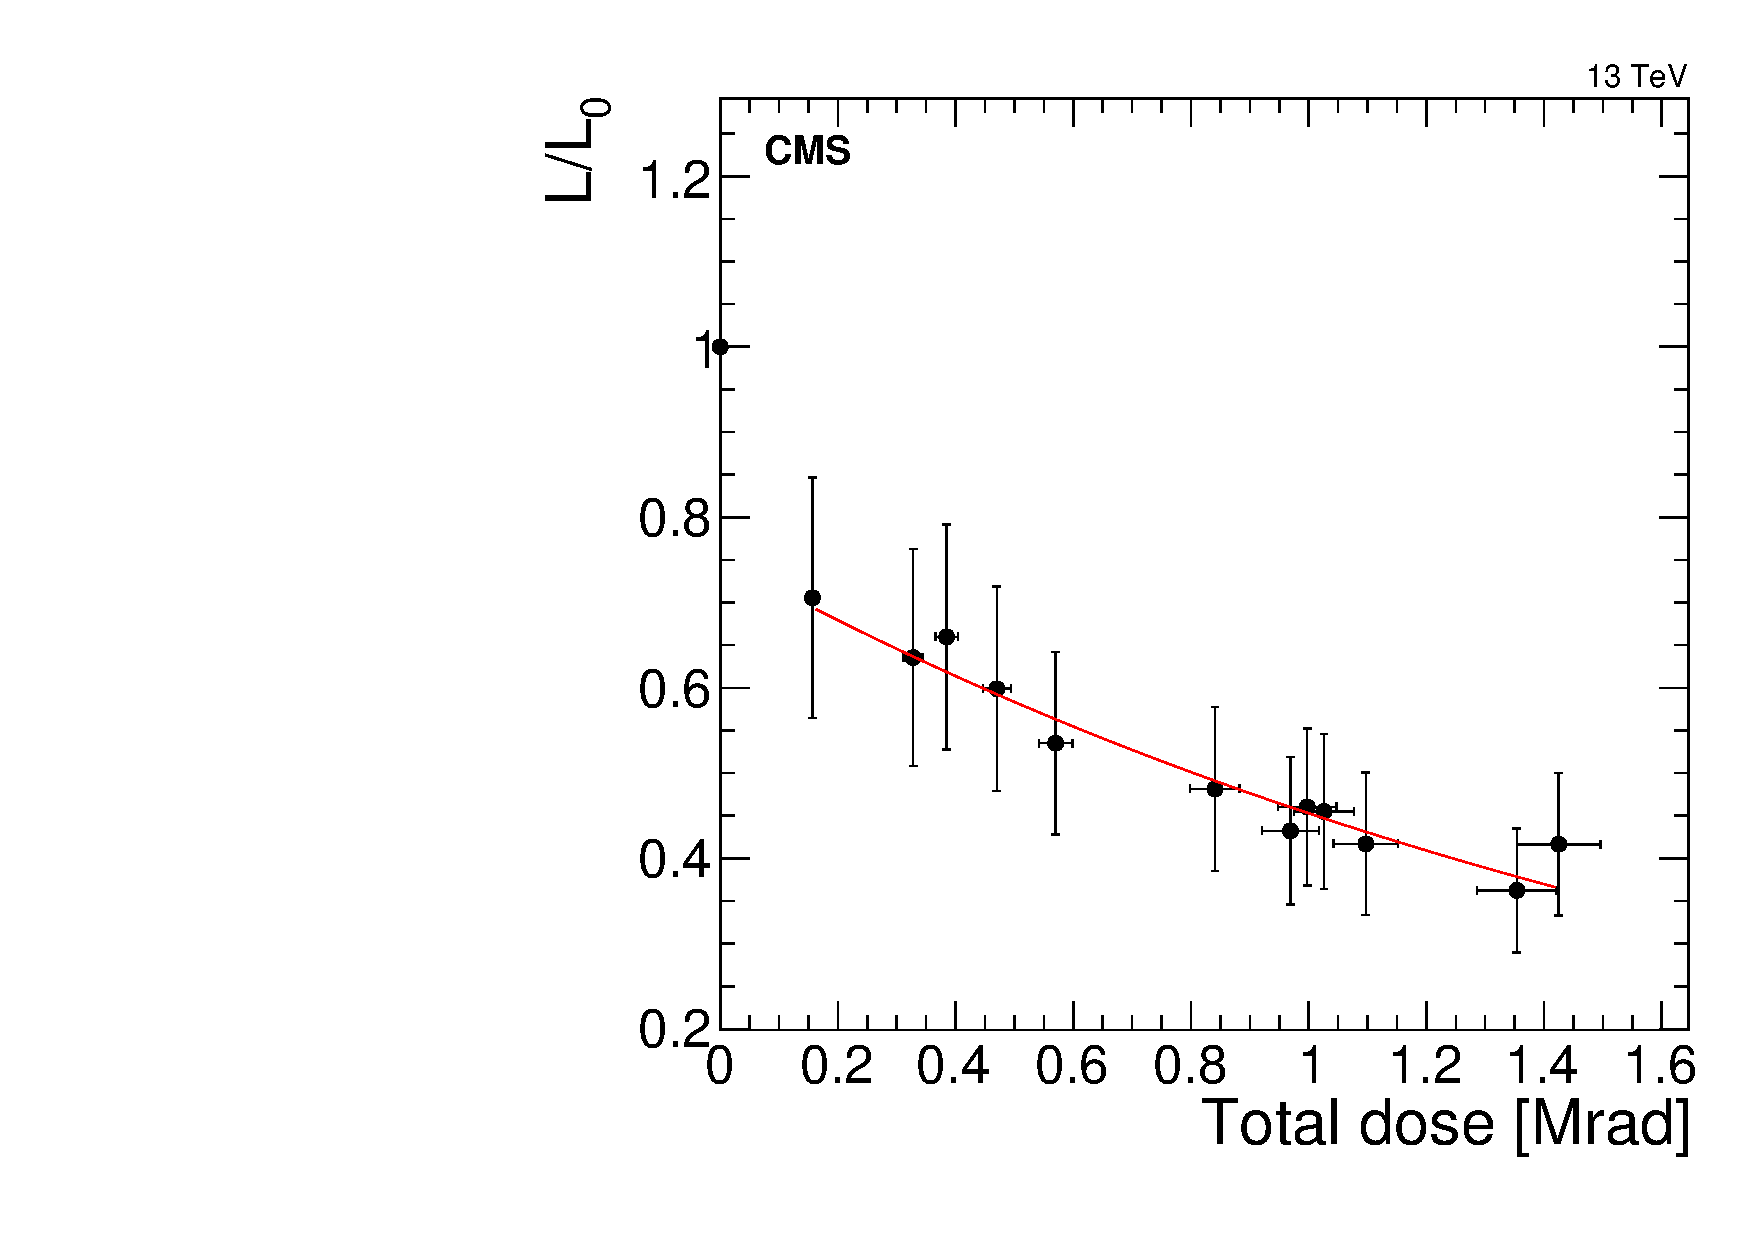
\includegraphics[width=0.32\textwidth]{figures/SCSN81-F-27p2cm-f6ch1-dose.pdf}
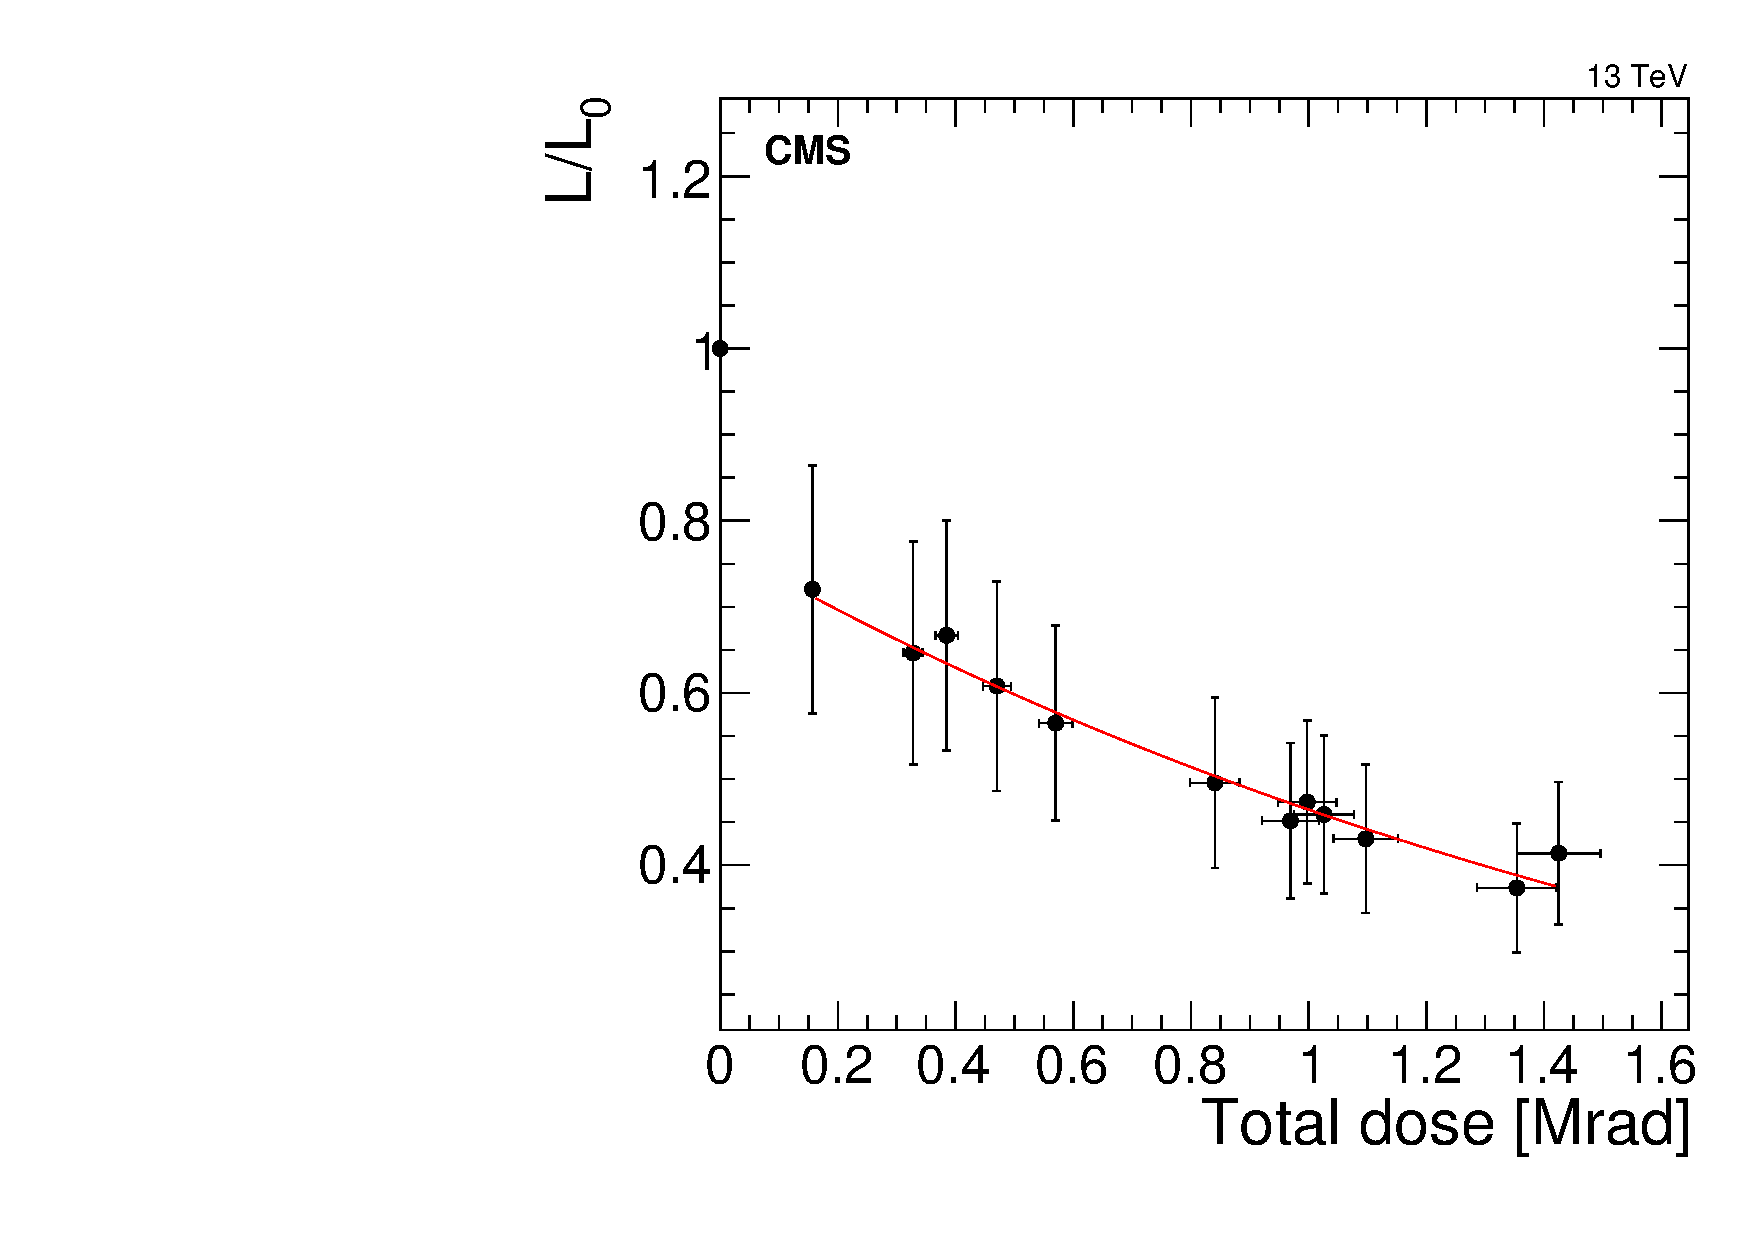
\includegraphics[width=0.32\textwidth]{figures/SCSN81-F-27p2cm-f8ch4-dose.pdf}
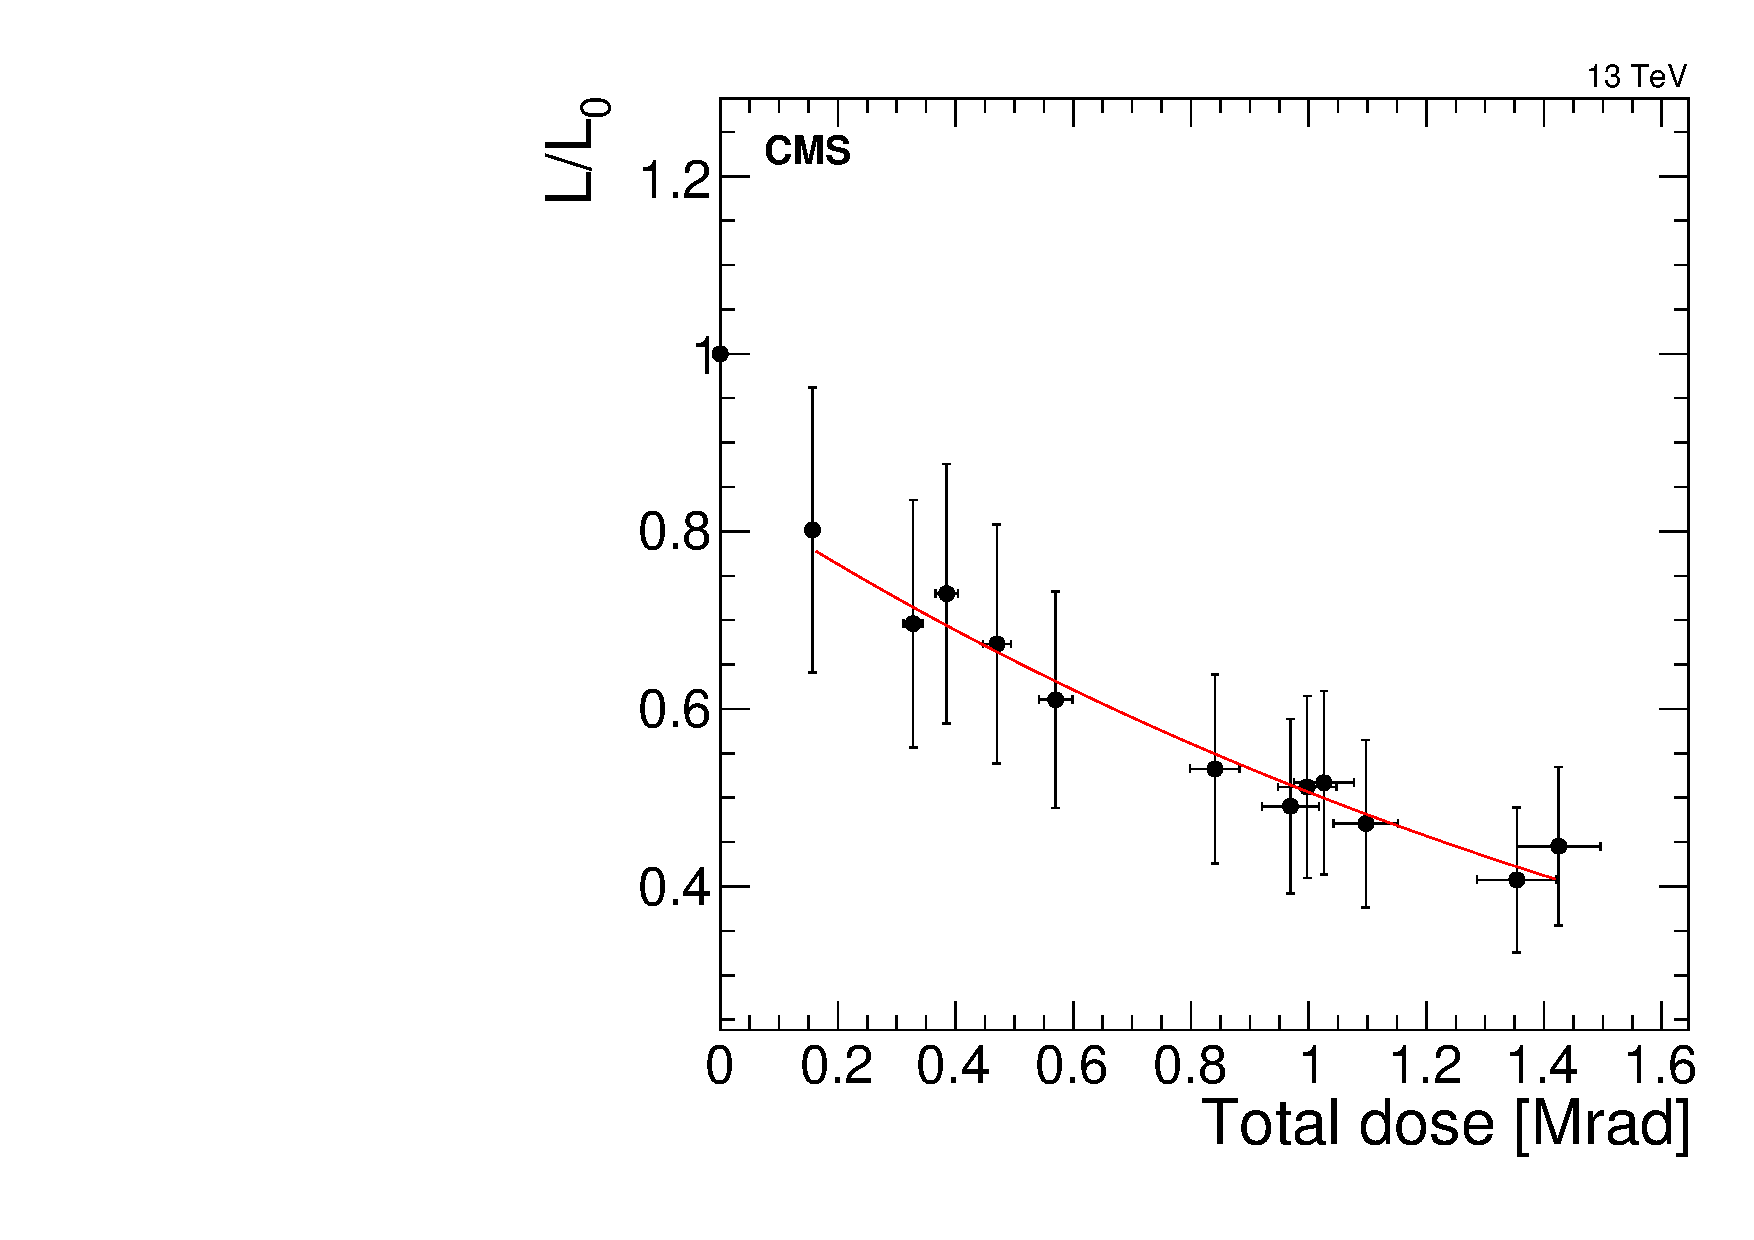
\includegraphics[width=0.32\textwidth]{figures/SCSN81-F-27p2cm-f14ch2-dose.pdf}
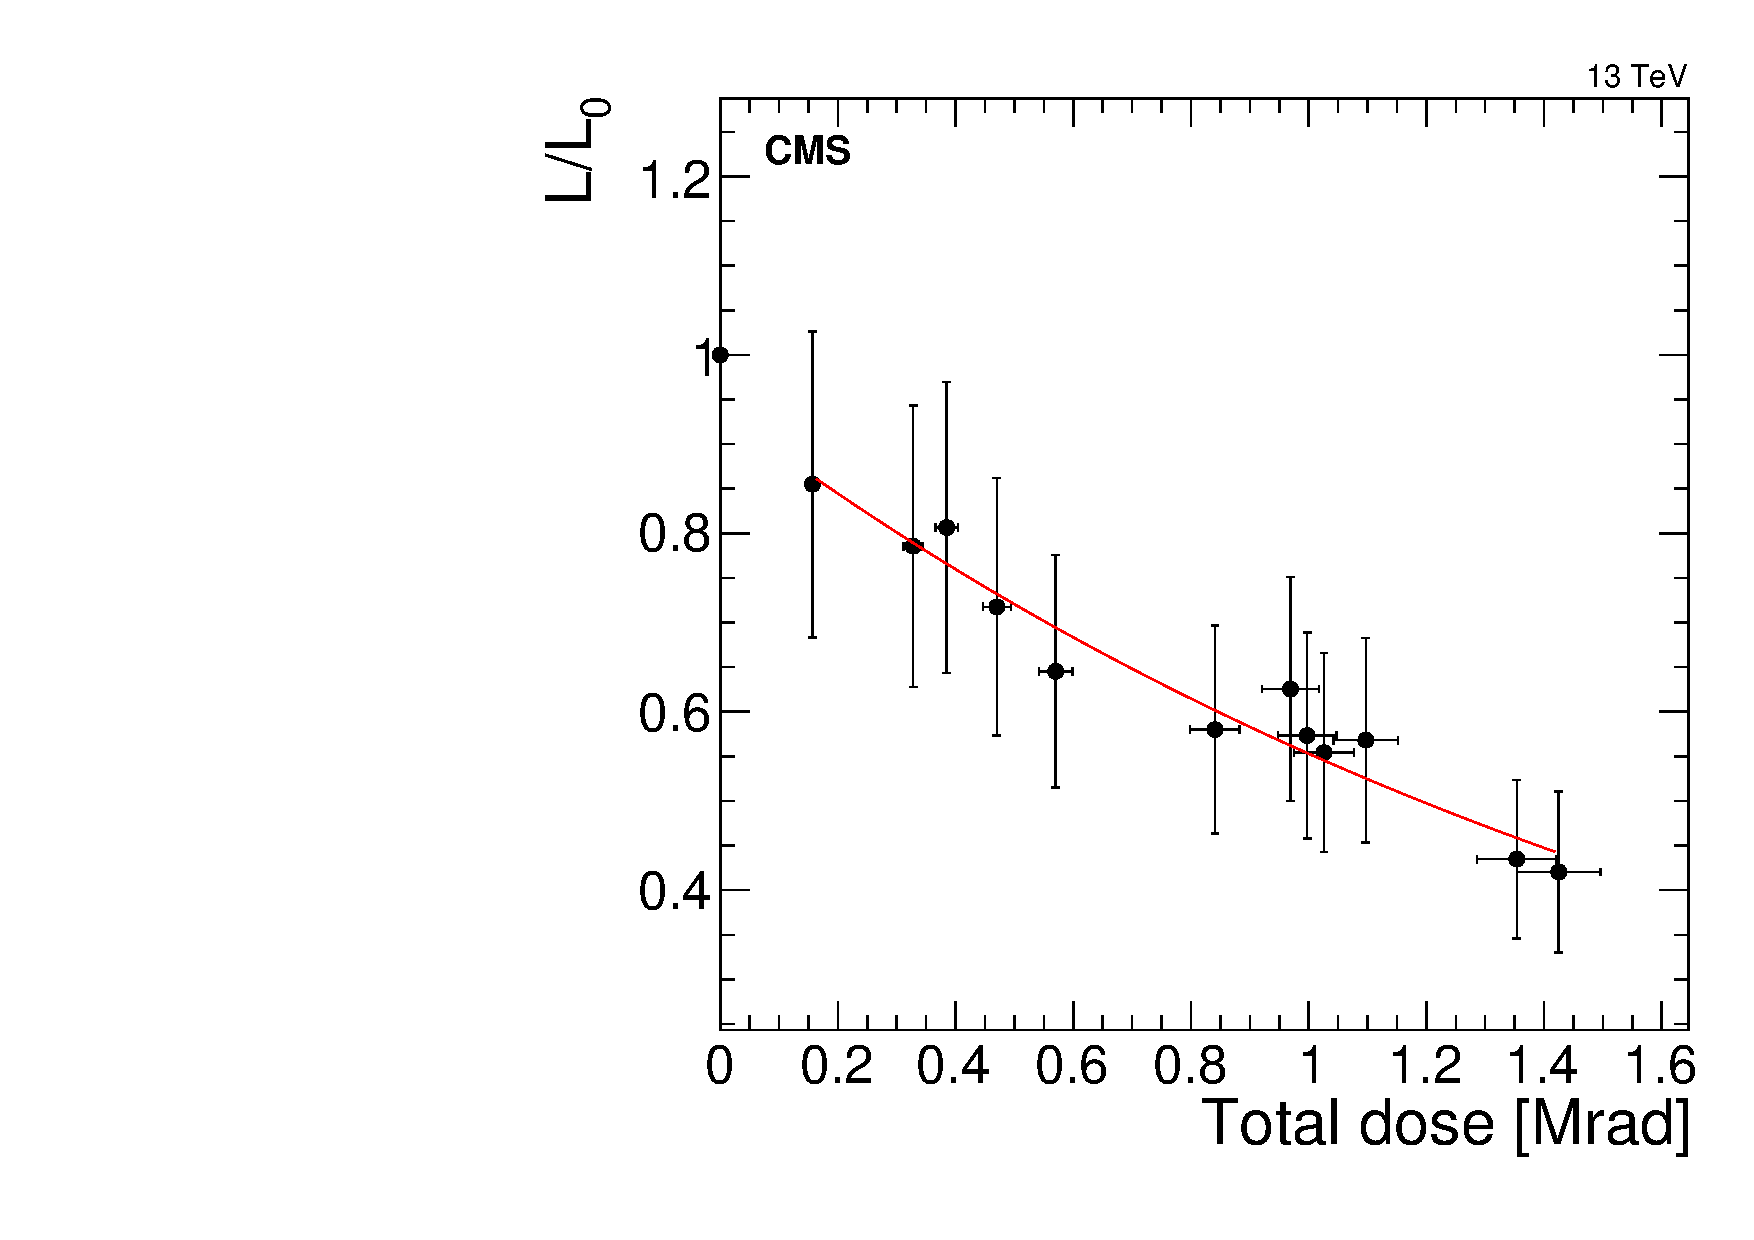
\includegraphics[width=0.32\textwidth]{figures/SCSN81-F-27p2cm-f14ch5-dose.pdf}
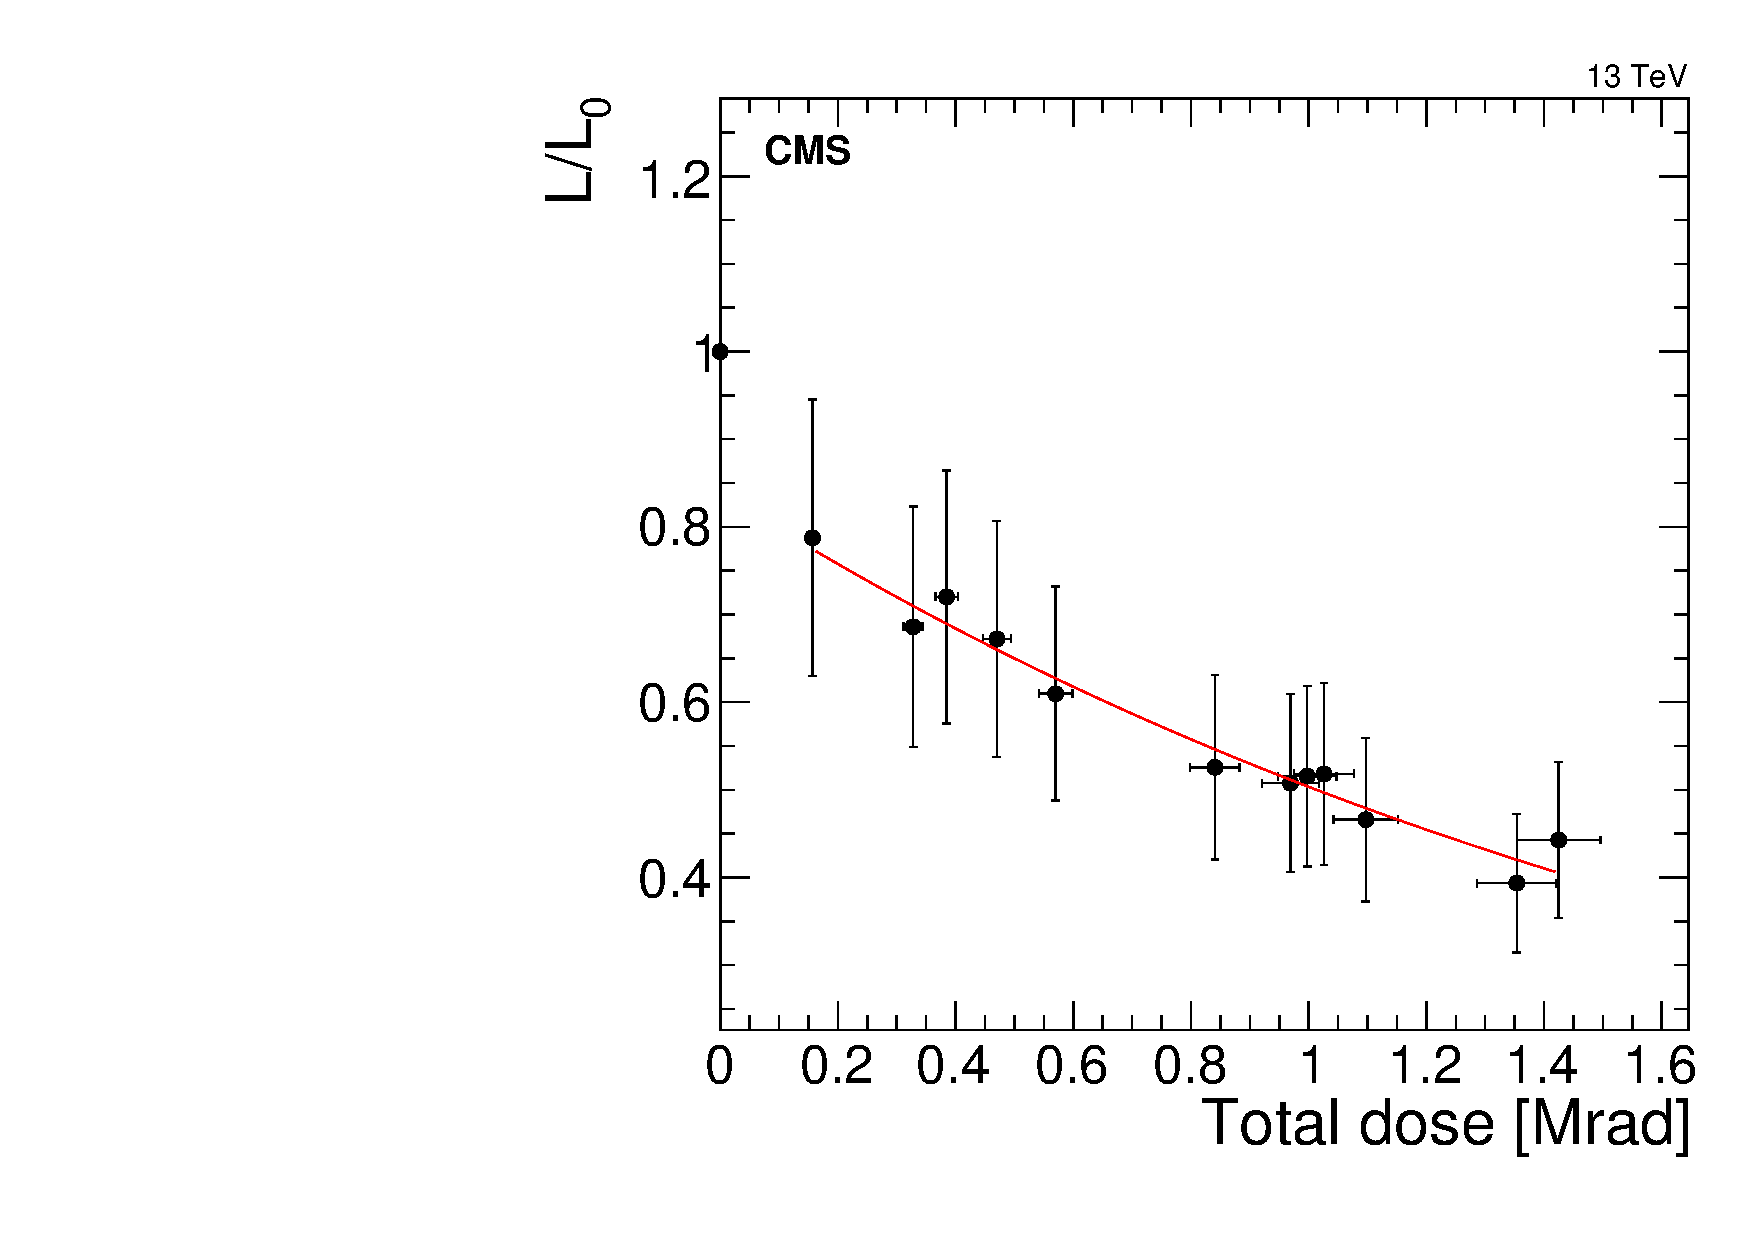
\includegraphics[width=0.32\textwidth]{figures/SCSN81-F-27p2cm-f16ch0-dose.pdf}
\caption{Relative yield versus integrated dose for SCSN81 finger tiles at 27.2 cm from the CMS beam pipe, receiving 3.93 krad/hr. The exponential decay curve fitted to the steady-state region of light loss is shown in red.}
\label{fig:SCSN81-F-27p2cm-dose}
\end{figure} 

\begin{figure}[tbp!]
\centering
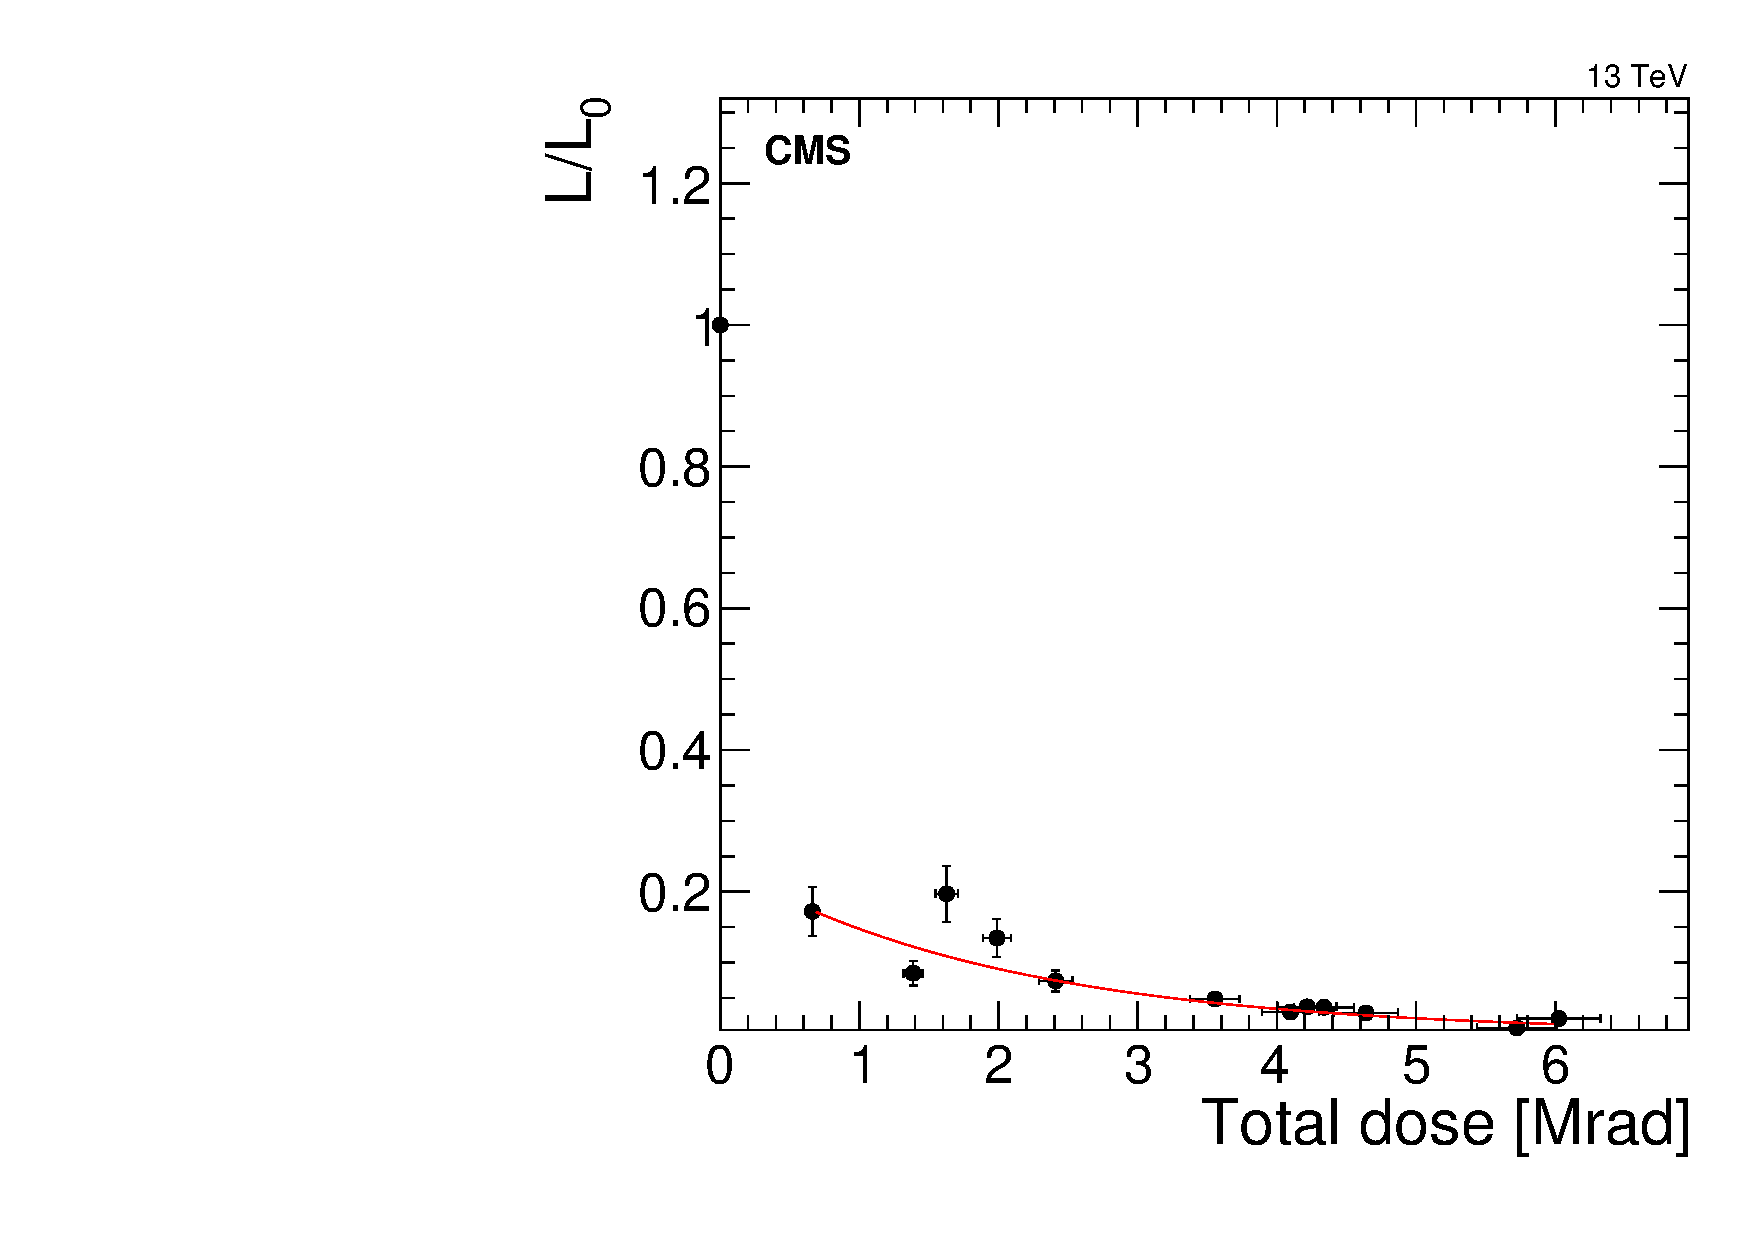
\includegraphics[width=0.45\textwidth]{figures/EJ200-S-11p8cm-f18ch5-dose.pdf}
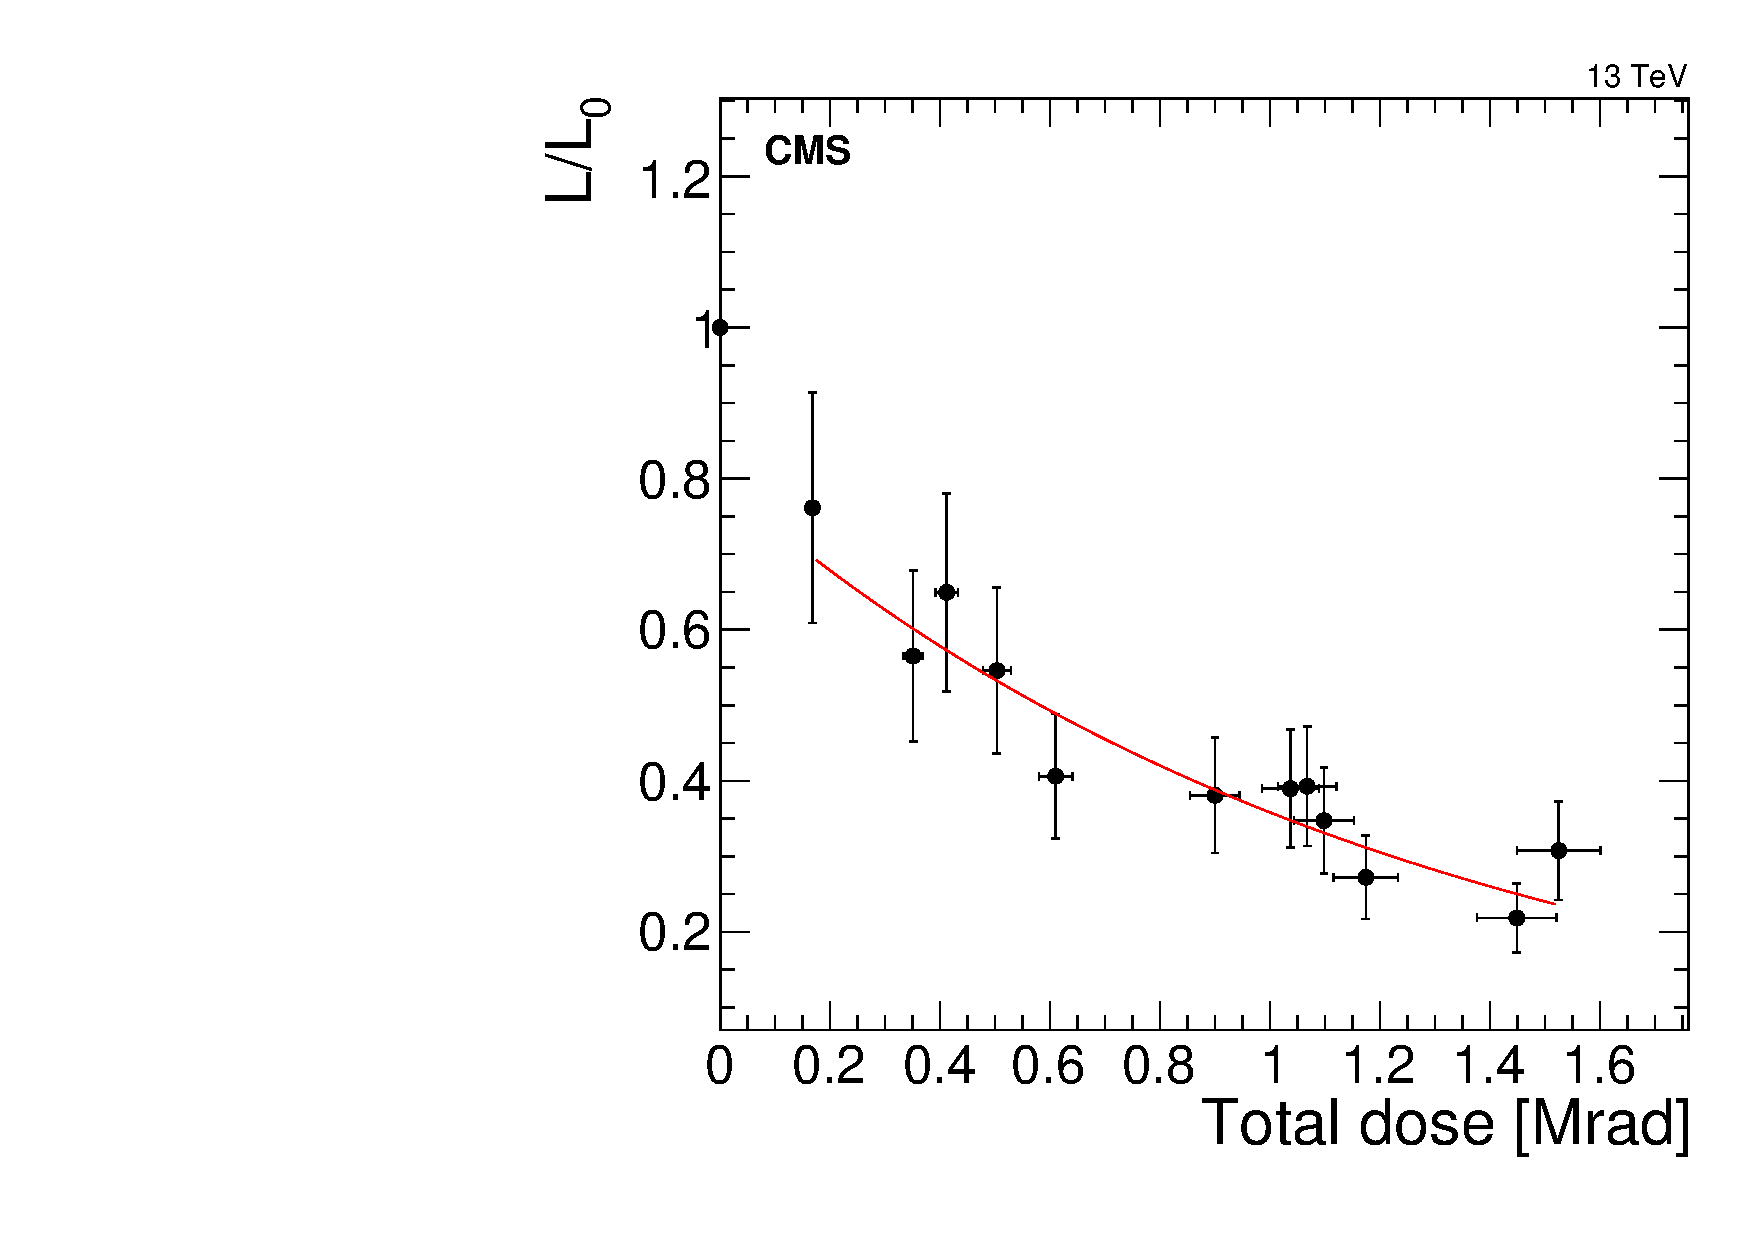
\includegraphics[width=0.45\textwidth]{figures/EJ200-S-25p9cm-f15ch5-dose.pdf}
\caption{Relative yield versus integrated dose for EJ200 sigma tiles. (\cmsLeft) Tile at 11.8 cm from the CMS beam pipe, receiving 16.61 krad/hr. (\cmsRight) Tile at 25.9 cm from the beam pipe, receiving 4.20 krad/hr. The exponential decay curve fitted to the steady-state region of light loss is shown in red.}
\label{fig:EJ200-S-dose}
\end{figure} 

\begin{figure}[tbp!]
\centering
\includegraphics[width=0.45\textwidth]{figures/EJ260-S-11p8cm-f8ch2-dose.pdf}
\includegraphics[width=0.45\textwidth]{figures/EJ260-S-18p2cm-f3ch1-dose.pdf}
\caption{Relative yield versus integrated dose for EJ260 sigma tiles. (\cmsLeft) Tile at 11.8 cm from the CMS beam pipe, receiving 16.61 krad/hr. (\cmsRight) Tile at 18.2 cm from the beam pipe, receiving 6.89 krad/hr. The exponential decay curve fitted to the steady-state region of light loss is shown in red.}
\label{fig:EJ260-S-dose}
\end{figure} 

\begin{figure}[tbp!]
\centering
\includegraphics[width=0.45\textwidth]{figures/EJ260-F-14p4cm-f6ch0-dose.pdf}
\includegraphics[width=0.45\textwidth]{figures/EJ260-F-14p4cm-f8ch1-dose.pdf}
\includegraphics[width=0.45\textwidth]{figures/EJ260-F-20p8cm-f3ch4-dose.pdf}
\includegraphics[width=0.45\textwidth]{figures/EJ260-F-20p8cm-f7ch1-dose.pdf}
\includegraphics[width=0.45\textwidth]{figures/EJ260-F-27p2cm-f8ch3-dose.pdf}
\caption{Relative yield versus integrated dose for EJ260 finger tiles. Top left and right: tiles at 14.4 cm from the CMS beam pipe, receiving 13.44 krad/hr. Middle left and right: tiles at 20.8 cm from the beam pipe, receiving 5.65 krad/hr. Bottom: tile at 27.2 cm from the beam pipe, receiving 3.93 krad/hr. The exponential decay curve fitted to the steady-state region of light loss is shown in red.}
\label{fig:EJ260-F-dose}
\end{figure} 


\subsubsection{Light yield versus time\label{sec:ana-res-lyvstime}}

The relative light yields for the various tiles as a function of the number of days after the start of irradiation are shown here in Figures~\ref{fig:SCSN81-S-11p8cm-time} to~\ref{fig:EJ260-F-time}. Day 0 refers to the day when the tiles were installed on the CASTOR table, before irradiation. Irradiation began on day 2 and ended on day 42, after which some recovery in the relative light yield can be observed in most of the tiles.

\begin{figure}[tbp!]
\centering
\includegraphics[width=0.45\textwidth]{figures/SCSN81-S-11p8cm-f3ch0-time.pdf}
\includegraphics[width=0.45\textwidth]{figures/SCSN81-S-11p8cm-f20ch1-time.pdf}
\includegraphics[width=0.45\textwidth]{figures/SCSN81-S-13p1cm-f7ch5-time.pdf}
\caption{Relative yield versus time for SCSN81 sigma tiles at 11.8 cm (top left and right) and 13.1 cm (bottom) from the CMS beam pipe, receiving 16.61 krad/hr and 15.23 krad/hr respectively. Irradiation began on day 2 and ended on day 42.}
\label{fig:SCSN81-S-11p8cm-time}
\end{figure} 

\begin{figure}[tbp!]
\centering
\includegraphics[width=0.45\textwidth]{figures/SCSN81-S-18p2cm-f5ch0-time.pdf}
\includegraphics[width=0.45\textwidth]{figures/SCSN81-S-18p2cm-f20ch5-time.pdf}
\caption{Relative yield versus time for SCSN81 sigma tiles at 18.2 cm from the CMS beam pipe, receiving 6.89 krad/hr. Irradiation began on day 2 and ended on day 42.}
\label{fig:SCSN81-S-18p2cm-time}
\end{figure} 

\begin{figure}[tbp!]
\centering
\includegraphics[width=0.45\textwidth]{figures/SCSN81-S-19p5cm-f2ch1-time.pdf}
\includegraphics[width=0.45\textwidth]{figures/SCSN81-S-19p5cm-f15ch1-time.pdf}
\includegraphics[width=0.45\textwidth]{figures/SCSN81-S-19p5cm-f20ch4-time.pdf}
\caption{Relative yield versus time for SCSN81 sigma tiles at 19.5 cm from the CMS beam pipe, receiving 5.86 krad/hr. Irradiation began on day 2 and ended on day 42.}
\label{fig:SCSN81-S-19p5cm-time}
\end{figure} 

\begin{figure}[tbp!]
\centering
\includegraphics[width=0.45\textwidth]{figures/SCSN81-S-24p6cm-f3ch2-time.pdf}
\includegraphics[width=0.45\textwidth]{figures/SCSN81-S-24p6cm-f14ch4-time.pdf}
\includegraphics[width=0.45\textwidth]{figures/SCSN81-S-24p6cm-f15ch4-time.pdf}
\caption{Relative yield versus time for SCSN81 sigma tiles at 24.6 cm from the CMS beam pipe, receiving 4.82 krad/hr. Irradiation began on day 2 and ended on day 42.}
\label{fig:SCSN81-S-24p6cm-time}
\end{figure} 

\begin{figure}[tbp!]
\centering
\includegraphics[width=0.45\textwidth]{figures/SCSN81-S-25p9cm-f7ch2-time.pdf}
\includegraphics[width=0.45\textwidth]{figures/SCSN81-S-25p9cm-f8ch5-time.pdf}
\includegraphics[width=0.45\textwidth]{figures/SCSN81-S-25p9cm-f14ch3-time.pdf}
\includegraphics[width=0.45\textwidth]{figures/SCSN81-S-25p9cm-f16ch1-time.pdf}
\caption{Relative yield versus time for SCSN81 sigma tiles at 25.9 cm from the CMS beam pipe, receiving 4.20 krad/hr. Irradiation began on day 2 and ended on day 42.}
\label{fig:SCSN81-S-25p9cm-time}
\end{figure} 

\begin{figure}[tbp!]
\centering
\includegraphics[width=0.45\textwidth]{figures/SCSN81-F-14p4cm-f4ch3-time.pdf}
\includegraphics[width=0.45\textwidth]{figures/SCSN81-F-14p4cm-f7ch0-time.pdf}
\includegraphics[width=0.45\textwidth]{figures/SCSN81-F-14p4cm-f18ch0-time.pdf}
\includegraphics[width=0.45\textwidth]{figures/SCSN81-F-14p4cm-f18ch1-time.pdf}
\includegraphics[width=0.45\textwidth]{figures/SCSN81-F-14p4cm-f18ch2-time.pdf}
\caption{Relative yield versus time for SCSN81 finger tiles at 14.4 cm from the CMS beam pipe, receiving 13.44 krad/hr. Irradiation began on day 2 and ended on day 42.}
\label{fig:SCSN81-F-14p4cm-time}
\end{figure} 

\begin{figure}[tbp!]
\centering
\includegraphics[width=0.45\textwidth]{figures/SCSN81-F-20p8cm-f2ch0-time.pdf}
\includegraphics[width=0.45\textwidth]{figures/SCSN81-F-20p8cm-f4ch1-time.pdf}
\includegraphics[width=0.45\textwidth]{figures/SCSN81-F-20p8cm-f15ch2-time.pdf}
\includegraphics[width=0.45\textwidth]{figures/SCSN81-F-20p8cm-f15ch3-time.pdf}
\includegraphics[width=0.45\textwidth]{figures/SCSN81-F-20p8cm-f20ch2-time.pdf}
\includegraphics[width=0.45\textwidth]{figures/SCSN81-F-20p8cm-f20ch3-time.pdf}
\caption{Relative yield versus time for SCSN81 finger tiles at 20.8 cm from the CMS beam pipe, receiving 5.65 krad/hr. Irradiation began on day 2 and ended on day 42.}
\label{fig:SCSN81-F-20p8cm-time}
\end{figure} 

\begin{figure}[tbp!]
\centering
\includegraphics[width=0.32\textwidth]{figures/SCSN81-F-27p2cm-f2ch5-time.pdf}
\includegraphics[width=0.32\textwidth]{figures/SCSN81-F-27p2cm-f3ch5-time.pdf}
\includegraphics[width=0.32\textwidth]{figures/SCSN81-F-27p2cm-f4ch0-time.pdf}
\includegraphics[width=0.32\textwidth]{figures/SCSN81-F-27p2cm-f6ch1-time.pdf}
\includegraphics[width=0.32\textwidth]{figures/SCSN81-F-27p2cm-f8ch4-time.pdf}
\includegraphics[width=0.32\textwidth]{figures/SCSN81-F-27p2cm-f14ch2-time.pdf}
\includegraphics[width=0.32\textwidth]{figures/SCSN81-F-27p2cm-f14ch5-time.pdf}
\includegraphics[width=0.32\textwidth]{figures/SCSN81-F-27p2cm-f16ch0-time.pdf}
\caption{Relative yield versus time for SCSN81 finger tiles at 27.2 cm from the CMS beam pipe, receiving 3.93 krad/hr. Irradiation began on day 2 and ended on day 42.}
\label{fig:SCSN81-F-27p2cm-time}
\end{figure} 

\begin{figure}[tbp!]
\centering
\includegraphics[width=0.45\textwidth]{figures/EJ200-S-11p8cm-f18ch5-time.pdf}
\includegraphics[width=0.45\textwidth]{figures/EJ200-S-25p9cm-f15ch5-time.pdf}
\caption{Relative yield versus time for EJ200 sigma tiles. (\cmsLeft) Tile at 11.8 cm from the CMS beam pipe, receiving 16.61 krad/hr. (\cmsRight) Tile at 25.9 cm from the beam pipe, receiving 4.20 krad/hr. Irradiation began on day 2 and ended on day 42.}
\label{fig:EJ200-S-time}
\end{figure} 

\begin{figure}[tbp!]
\centering
\includegraphics[width=0.45\textwidth]{figures/EJ260-S-11p8cm-f8ch2-time.pdf}
\includegraphics[width=0.45\textwidth]{figures/EJ260-S-18p2cm-f3ch1-time.pdf}
\caption{Relative yield versus time for EJ260 sigma tiles. (\cmsLeft) Tile at 11.8 cm from the CMS beam pipe, receiving 16.61 krad/hr. (\cmsRight) Tile at 18.2 cm from the beam pipe, receiving 6.89 krad/hr. Irradiation began on day 2 and ended on day 42.}
\label{fig:EJ260-S-time}
\end{figure} 

\begin{figure}[tbp!]
\centering
\includegraphics[width=0.45\textwidth]{figures/EJ260-F-14p4cm-f6ch0-time.pdf}
\includegraphics[width=0.45\textwidth]{figures/EJ260-F-14p4cm-f8ch1-time.pdf}
\includegraphics[width=0.45\textwidth]{figures/EJ260-F-20p8cm-f3ch4-time.pdf}
\includegraphics[width=0.45\textwidth]{figures/EJ260-F-20p8cm-f7ch1-time.pdf}
\includegraphics[width=0.45\textwidth]{figures/EJ260-F-27p2cm-f8ch3-time.pdf}
\caption{Relative yield versus time for EJ260 finger tiles. Top left and right: tiles at 14.4 cm from the CMS beam pipe, receiving 13.44 krad/hr. Middle left and right: tiles at 20.8 cm from the beam pipe, receiving 5.65 krad/hr. Bottom: tile at 27.2 cm from the beam pipe, receiving 3.93 krad/hr. Irradiation began on day 2 and ended on day 42.}
\label{fig:EJ260-F-time}
\end{figure} 

\subsubsection{Tables of dose constants\label{sec:ana-res-tables}}
The dose constants calculated for the SCSN81 sigma tiles, SCSN81 finger tiles, EJ200/EJ260 tiles, and special tiles are summarized in Tables~\ref{tab:SCSN81-S},~\ref{tab:SCSN81-F},~\ref{tab:EJs},and~\ref{tab:special} respectively.

\begin{table}[htbh]
\begin{center}
\topcaption{Dose constants for SCSN81 sigma tiles. In the case where more than one tile was at the same distance from the beam pipe and thus receiving the same dose rate, the dose constant for that dose rate is taken to be the weighted average of the dose constants calculated for those tiles.\label{tab:SCSN81-S}}
\begin{tabular}{|c|c|c|c|}
\hline
Distance (cm) & Dose rate (krad/hr) & Total dose (Mrad) & Dose constant (Mrad)\\
\hline
\hline
11.8 & 16.61 & 6.04 & 6.58 $\pm$ 1.13\\
13.1 & 15.23 & 5.54 & 6.55 $\pm$ 1.89\\
18.2 & 6.89 & 2.51 & 4.37 $\pm$ 1.30\\
19.5 & 5.86 & 2.13 & 4.24 $\pm$ 1.16\\
24.6 & 4.82 & 1.75 & 4.08 $\pm$ 1.05\\
25.9 & 4.20 & 1.53 & 3.12 $\pm$ 0.57\\
\hline
\end{tabular}
\end{center}
\end{table}

% To add: SCSN81 finger tiles

\begin{table}[htbh]
\begin{center}
\topcaption{Dose constants for SCSN81 finger tiles.\label{tab:SCSN81-F}}
\begin{tabular}{|c|c|c|c|}
\hline
Distance (cm) & Dose rate (krad/hr) & Total dose (Mrad) & Dose constant (Mrad)\\
\hline
\hline
14.4 & 13.44 & 4.89 & 7.32 $\pm$ 1.73\\
14.4 & 13.44 & 4.89 & 7.47 $\pm$ 1.77\\
14.4 & 13.44 & 4.89 & 9.34 $\pm$ 2.87\\
14.4 & 13.44 & 4.89 & 9.07 $\pm$ 2.72\\
14.4 & 13.44 & 4.89 & 8.72 $\pm$ 2.49\\
20.8 & 5.65 & 2.06 & 4.18 $\pm$ 1.44\\
20.8 & 5.65 & 2.06 & 4.0 $\pm$ 1.29\\
20.8 & 5.65 & 2.06 & 4.91 $\pm$ 2.01\\
20.8 & 5.65 & 2.06 & 5.10 $\pm$ 2.18\\
20.8 & 5.65 & 2.06 & 4.35 $\pm$ 1.55\\
20.8 & 5.65 & 2.06 & 4.28 $\pm$ 1.51\\
27.2 & 3.93 & 1.43 & 3.17 $\pm$ 1.20\\
27.2 & 3.93 & 1.43 & 3.35 $\pm$ 1.33\\
27.2 & 3.93 & 1.43 & 3.34 $\pm$ 1.31\\
27.2 & 3.93 & 1.43 & 3.36 $\pm$ 1.33\\
27.2 & 3.93 & 1.43 & 3.40 $\pm$ 1.36\\
27.2 & 3.93 & 1.43 & 3.93 $\pm$ 1.94\\
27.2 & 3.93 & 1.43 & 3.47 $\pm$ 1.53\\
27.2 & 3.93 & 1.43 & 3.72 $\pm$ 1.71\\
\hline
\end{tabular}
\end{center}
\end{table}

\begin{table}[htbh]
\begin{center}
\topcaption{Dose constants for EJ200 and EJ260 tiles.\label{tab:EJs}}
\begin{tabular}{|c|c|c|c|c|}
\hline
Type & Distance (cm) & Dose rate (krad/hr) & Total dose (Mrad) & Dose constant (Mrad)\\
\hline
\hline
EJ200 sigma & 11.8 & 16.61 & 6.04 & 7.54 $\pm$ 1.26\\
EJ200 sigma & 25.9 & 4.20 & 1.53 & 2.36 $\pm$ 0.59\\
EJ260 sigma & 11.8 & 16.61 & 6.04 & 35.88 $\pm$ 31.34\\
EJ260 sigma & 11.8 & 16.61 & 6.04 & 29.06 $\pm$ 25.49\\
EJ260 sigma & 18.2 & 6.89 & 2.51 & 6.02 $\pm$ 2.14\\
EJ260 finger & 14.4 & 13.44 & 4.89 & 15.20 $\pm$ 7.09\\
EJ260 finger & 14.4 & 13.44 & 4.89 & 17.62 $\pm$ 9.39\\
EJ260 finger & 20.8 & 5.65 & 2.06 & 7.64 $\pm$ 4.62\\
EJ260 finger & 20.8 & 5.65 & 2.06 & 6.91 $\pm$ 3.69\\
EJ260 finger & 27.2 & 3.93 & 1.43 & 7.57 $\pm$ 6.96\\
\hline
\end{tabular}
\end{center}
\end{table}

\begin{table}[htbh]
\begin{center}
\topcaption{Dose constants for tiles with special materials or shapes. N.B.: only some of the tiles from the initial list are shown here. Several had to be omitted from the dose constant calculation due to either a lack of a non-irradiated day 0 measurement (because of data link instabilities on the first day), or to the fact that the tile was damaged too much by radiation to have a readable signal in the end.\label{tab:special}}
\begin{tabular}{|c|c|c|c|c|}
\hline
Type & Distance (cm) & Dose rate (krad/hr) & Total dose (Mrad) & Dose constant (Mrad)\\
\hline
\hline
LS6946 finger & 27.2 & 3.93 & 1.43 & 2.55 $\pm$ 0.75\\
Scintillator X & 13.1 & 15.23 & 5.54 & 11.43 $\pm$ 3.67\\
PEN & 13.1 & 15.23 & 5.54 & 12.34 $\pm$ 5.33\\
PEN & 13.1 & 15.23 & 5.54 & 11.82 $\pm$ 4.28\\
\hline
\end{tabular}
\end{center}
\end{table}


%\subsubsection{Radiation damage\label{sec:ana-raddam}}

%\subsubsection{Recovery\label{sec:ana-recovery}}

\subsubsection{Dark current\label{sec:ana-dark}}

%\subsubsection{Dose rate effect\label{sec:ana-doseconst}}
